% for the article version
%\documentclass{article}
%\usepackage{beamerarticle}

% for the beamer version
\documentclass[t,8pt]{beamer}%{beamer}%{article} 9pt
%\usetheme{simpleplus}
\usetheme{}
%\usecolortheme{structure}
\AtBeginSection[]{
	\begin{frame}
		\vfill
		\centering
		\begin{beamercolorbox}[sep=8pt,center,shadow=true,rounded=true]{title}
			\usebeamerfont{title}\insertsectionhead\par%
		\end{beamercolorbox}
		\vfill
	\end{frame}
}

\definecolor{davered}{rgb}{.5,0,0}
%
%\setbeamercolor{normal text}{fg=white,bg=black!90}
%\setbeamercolor{structure}{fg=white}
%
\setbeamercolor{normal text}{fg=black!90,bg=NavyBlue!5}
\setbeamercolor{structure}{fg=black!90}

\setbeamercolor{alerted text}{fg=red!85!black}
\setbeamercolor{item projected}{use=item,fg=black,bg=item.fg!35}
\setbeamercolor*{palette primary}{use=structure,fg=structure.fg}
\setbeamercolor*{palette secondary}{use=structure,fg=structure.fg!95!black}
\setbeamercolor*{palette tertiary}{use=structure,fg=structure.fg!90!black}
\setbeamercolor*{palette quaternary}{use=structure,fg=structure.fg!95!black,bg=black!80}
\setbeamercolor*{framesubtitle}{fg=white}
\setbeamercolor*{block title}{parent=structure,bg=black!60}
\setbeamercolor*{block body}{fg=black,bg=black!10}
\setbeamercolor*{block title alerted}{parent=alerted text,bg=black!15}
\setbeamercolor*{block title example}{parent=example text,bg=black!15}

%Packages
\usepackage{amsmath}
\usepackage{mathtools}
\usepackage[skip=5pt plus1pt, indent=0pt]{parskip}
%\usepackage{xcolor}
\usepackage[dvipsnames]{xcolor}
\usepackage{comment}
\usepackage{tikz}
%\usetikzlibrary{arrows}
\usetikzlibrary{decorations.pathreplacing,calc,positioning}
\usetikzlibrary{intersections}
%For 2x2 box - changed global font:
\usetikzlibrary{shapes,arrows,shadows}
\usepackage{amsmath,bm,times}
\usepackage[table,xcdraw]{xcolor}
\usepackage{array,multirow,graphicx}
\usepackage{pgfplots}
\usetikzlibrary{shapes, arrows, positioning}
%
\usepackage[most]{tcolorbox}
\usepackage{filecontents}
\usepackage{mathtools}

\tcbset{colback=NavyBlue!5, colframe=NavyBlue, 
	highlight math style= {enhanced, %<-- needed for the ’remember’ options
		colframe=red,colback=red!10!white,boxsep=0pt}
}
\setlength{\fboxrule}{1pt}
\setlength{\fboxsep}{0pt}

\usefonttheme{serif}

%%%%%%%%%%%%%%%%%%%%%%%%%%%%%%%%%%%%%%%%%%%%%%%%%%%%%%%%%%%%%%%%

% Theme and color adjustments (minimal)
\usetheme{default}
\setbeamersize{text margin left=.5cm, text margin right=4cm} % ← Key change for annotation space

% Optional: define a shaded annotation area
\usepackage{tcolorbox}
\tcbuselibrary{skins}
\newtcolorbox{marginannotation}[1][]{%
  enhanced,
  colback=yellow!5,
  colframe=yellow!50!black,
  width=4.5cm,
  left=1mm,
  right=1mm,
  boxrule=0.5pt,
  fonttitle=\bfseries,
  title=Note,
  sharp corners,
  boxsep=1mm,
  #1
}

% Optional: avoid content overflow in annotation space
\usepackage{varwidth}

\usepackage{etoolbox}

% Hook to draw on each slide
\makeatletter
\patchcmd{\beamer@@frametitle}{\gdef\insertframetitle}%
{\gdef\insertframetitle%
	\begin{tikzpicture}[remember picture,overlay]
		\foreach \y in {0.5,1,...,7.5} {
			\draw[gray!30, thin] ([xshift=-1cm,yshift=\y cm]current page.east) -- ([xshift=-5cm,yshift=\y cm]current page.east);
		}
		\foreach \x in {1,...,4} {
			\draw[gray!30, thin] ([xshift=-\x cm,yshift=0.5cm]current page.north east) -- ([xshift=-\x cm,yshift=-7.5cm]current page.north east);
		}
\end{tikzpicture}}{}{}
\makeatother

%%%%%%%%%%%%%%%%%%%%%%%%%%%%%%%%%%%%%%%%%%%%%%%%%%%%%%%%%%%%%%%%

\newcounter{exercise}
\counterwithin{exercise}{section}
\begin{document}
\tableofcontents

	
	%%%%%%%%%%%%%%%%%%%%%%%%%%%%%%%%%%%%%%%%%%%%%%%%%%%%%%%%%%%%%%%%
	%%%%%%%%%%%%%%%%%%%%%%%%%%%%%%%%%%%%%%%%%%%%%%%%%%%%%%%%%%%%%%%%
	%\title{Introduction to statistics with R}
	%\begin{filecontents*}{week1.tex}
	%\end{filecontents*}
	
	%\begin{comment}
	\section{Week 1: random variables and data}
	%Descriptive statistics
	
	\begin{frame}
		\frametitle{What is statistics?}
		Easy answer: statistics is the collection, analysis, interpretation or explanation, and presentation of data \par
		We often use mathematical models to describe phenomena we observe \par
		{\bf This course: using probability densities to model populations that are sampled via data sets} \par
		There is {\bf huge} overlap between probability and statistics
	\end{frame}
	
	\begin{frame}
		\frametitle{Navigating MATH163}
		\begin{itemize}
			\item Lecture slides: core theory and examples \par 
			{\small\color{NavyBlue} - some more intuitive comments are made in small coloured text \par 
				- you should make additional notes yourself - it is very helpful for understanding the theory}
			\item Problem sheets and solutions
			\item A single folder containing all materials for R practicals \par 
			\begin{itemize}
				\item[-] All data sets as .csv files
				\item[-] A PDF question sheet
				\item[-] Week 1-5 answers in an R script
				\item[-] Week 6-10 answers in an R markdown document
			\end{itemize}
			\item Assessment
			\begin{itemize}
				\item[-] 2 M\"obius homeworks (weeks 6 and 11)
				\item[-] A final written exam
			\end{itemize}
		\end{itemize}
	\end{frame}
	
	\begin{frame}
		\frametitle{MATH163 housekeeping}
		\begin{itemize}
			\item Lecture slides: core theory and examples \par 
			\item David's email: d.haw@liverpool.ac.uk - expect a response within 48h
			\item Office hours: \par
			Tuesday 12:00 (in person/online), Thursday 11:00 (in person/online) \par
            Office 407 (maths building)
			\item Any issues or requests should be voiced as early as possibly in order to resolve them in a timely manner
			\item Lectures an problems classes will be merged \par
			- expect to attempt exercises in class when you see this picture:
			\begin{center}
				\fbox{\includegraphics[width=.2\textwidth]{countdown.jpg}}
			\end{center}
			\item It's up to you not to look at the answers before you try something
			\item R practicals are designed to function as independent work
		\end{itemize}
	\end{frame}
	
	
	\begin{frame}
		\frametitle{What is statistics?}
		\centering
		
		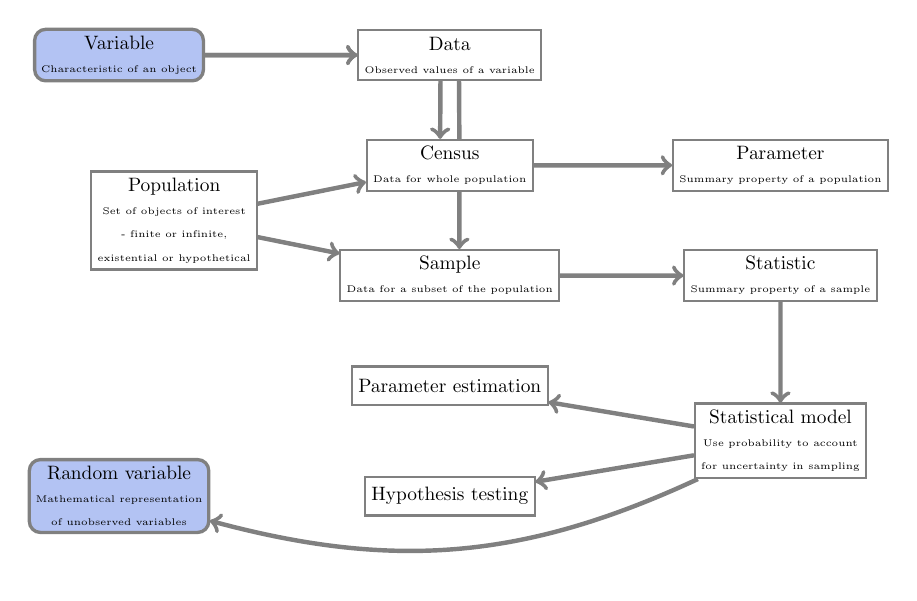
\begin{tikzpicture}[scale=.7,transform shape,thick,
			main node/.style={rectangle, draw=black!50, very thick, fill=RoyalBlue!40,align=center, text=black, rounded corners, minimum height=2em},%, text width=7em
			second node/.style={rectangle, draw=black!50, thick, fill=white, text=black, align=center, minimum height=2em,minimum width=25pt},
			third node/.style={rectangle, draw=black, thick, fill=blue!20, text width=6em,align=center, minimum height=2em,minimum width=25pt}]
			%\draw[teal,thick,fill=teal!10] (-1.7,1.3) rectangle (1.7,9.7);
			%\node[text=black,font=\small\sffamily] (1) at (-0,9.2) {OBSERVATIONS};
			%\node[text=black,font=\small\sffamily] (1) at (5,9.2) {ECON MODEL};
			%\node[text=black,font=\small\sffamily] (1) at (12,9.2) {EPI MODEL};
			
			\node[main node,minimum width=25pt] (1) at (0,10) {Variable\\{\tiny Characteristic of an object}};
			\node[second node] (2) at (6,10) {Data\\{\tiny Observed values of a variable}};
			\node[second node] (3) at (1,7) {Population\\{\tiny Set of objects of interest}\\{\tiny - finite or infinite,}\\{\tiny existential or hypothetical}};
			\node[second node] (4) at (6,8) {Census\\{\tiny Data for whole population}};
			\node[second node] (5) at (6,6) {Sample\\{\tiny Data for a subset of the population}};
			\node[second node] (6) at (12,8) {Parameter\\{\tiny Summary property of a population}};
			\node[second node] (7) at (12,6) {Statistic\\{\tiny Summary property of a sample}};
			%\node[second node,fill=white,minimum width=25pt] (1) at (12,4) {Probability\\{\tiny Represents uncertainty from sampling process}};
			\node[second node] (8) at (12,3) {Statistical model\\{\tiny Use probability to account}\\{\tiny for uncertainty in sampling}};
			\node[second node] (9) at (6,4) {Parameter estimation};
			\node[second node] (10) at (6,2) {Hypothesis testing};
			\node[main node] (11) at (0,2) {Random variable\\{\tiny Mathematical representation}\\{\tiny of unobserved variables}};
			
			\path[every node/.style={font=\sffamily\small}]
			(1) edge [line width=1pt,->,ultra thick, black!50] node[auto] {} (2)
			(2.250) edge [line width=1pt,->,ultra thick, black!50] node[auto] {} (4.110)
			(2.290) edge [line width=1pt,ultra thick, black!50] node[auto] {} (4.70)
			(4.290) edge [line width=1pt,->,ultra thick, black!50] node[auto] {} (5.70)
			(3) edge [line width=1pt,->,ultra thick, black!50] node[auto] {} (4)
			(3) edge [line width=1pt,->,ultra thick, black!50] node[auto] {} (5)
			(4) edge [line width=1pt,->,ultra thick, black!50] node[auto] {} (6)
			(5) edge [line width=1pt,->,ultra thick, black!50] node[auto] {} (7)
			(7) edge [line width=1pt,->,ultra thick, black!50] node[auto] {} (8)
			(8) edge [line width=1pt,->,ultra thick, black!50] node[auto] {} (9)
			(8) edge [line width=1pt,->,ultra thick, black!50] node[auto] {} (10)
			(8) edge [line width=1pt,->,ultra thick, black!50,bend left=20] node[auto] {} (11)
			
			(1) edge [line width=1pt,->,ultra thick, black!50] node[auto] {} (2);
			%(2) edge [line width=1pt,->,ultra thick,dashed] node[auto] {} (3)
			%(6) edge [line width=1pt,->,ultra thick] node[auto] {} (4)
			%(6) edge [line width=1pt,->,ultra thick] node[auto] {} (5)
			%(6) edge [line width=1pt,->,line width=3pt,color=violet!100,bend left=20] node[below left] {Contact rates} (2)%3
			
		\end{tikzpicture}
		
	\end{frame}
	
	\begin{frame}
		\frametitle{Data types}
		\begin{itemize}
			\item {\bf Qualitative:} categories/groups
			\begin{itemize}
				\item {\bf Categorical/nominal:} mutually exclusive, unordered \par
				Examples: sex, subject of study, hometown
				\item {\bf Ordinal:} mutually exclusive, order matters \par
				Examples: education level (BSc, MSc, PhD), military rank
			\end{itemize}
			\item {\bf Quantitative:} measured numerical values \par
			- ordinal by default
			\begin{itemize}
				\item {\bf Interval:} difference between $2$ values is meaningful \par
				Examples: temperature (Celsius/Farenheit), IQ score, time
				\item {\bf Ordinal:} zero means ``none" \par
				Examples: temperature (Kelvin), age, length
			\end{itemize}
			%\item Discrete/continuous: PMF (discrete) is ready-integrated; PDF (continuous) must be integrated to find probability; units; CDF
		\end{itemize}
	\end{frame}
	
	\begin{frame}
		\frametitle{Data types}
		\begin{itemize}
			\item {\bf Quantitative (continued):}
			\begin{itemize}
				\item {\bf Discrete:} data that are distinct, individual, and cannot be divided into smaller parts (countably many possible values) \par
				Examples: number of children, shoe size, age (years), outcome of rolling a dice
				\item {\bf Continuous:} data that can take any value in a given range (uncountably many possible values) \par
				Examples: temperature, foot size, luminosity, electrical power
			\end{itemize}
			%\item Discrete/continuous: PMF (discrete) is ready-integrated; PDF (continuous) must be integrated to find probability; units; CDF
		\end{itemize}
	\end{frame}
    
        \begin{frame}
		\frametitle{Data types}
        {\bf\underline{Exercise}} \par
        Classify the following variables using the terms \par
        qualitative (categorical/ordinal), quantitative (interval/ordinal, discrete/continuous):
        \begin{itemize}
            \item T-Shirt size (XS, S, M, L, XL) %Qual ordinal
            \item Moderated exam Score in MATH163 (0–100 scale) %Quant interval cont?
            \item Preferred Study Method (Group, Solo, Procrastination) %Qual cat
            \item Satisfaction with campus facilities \par
            (e.g., Very Dissatisfied, Dissatisfied, Neutral, Satisfied, Very Satisfied %Qual ordinal
            \item Number of classes taken this semester (USA) %Quant ordinal discrete
            \item Major/Field of Study %Qual cat
            \item Height of Students (in centimeters) %Quant cont
            \item Number of days absent from lectures in a month %Quant discrete
        \end{itemize}
		
	\end{frame}

    \begin{frame}
		\frametitle{Summary statistics: intuition}
		\begin{itemize}
			\item \tikz[remember picture] \node[coordinate,yshift=0.5em] (n1) {};{\bf Mean:} the ``centre of mass" of the data
			{\color{black!40}
				\item {\bf Mode:} the most common value
				\item {\bf Median:} the midpoint of the ordered data
				\item \tikz[remember picture] \node[coordinate] (n2) {};{\bf Percentiles} (typically $0,5,25,50,75,95,100$)
			}
			{\color{black!40}
				\item\tikz[remember picture] \node[coordinate,yshift=0.5em] (m1) {};{\bf Range:} difference between largest and smallest value
				\item {\bf Interquartile range:} $75$th-$25$th percentile
				\item {\bf Mean absolute deviation:} mean distance from the mean
			}
			\item {\bf Variance:} mean squared distance from the mean
			\item \tikz[remember picture] \node[coordinate] (m2) {};{\bf Standard deviation:} square root of variance
			{\color{black!40}
				\item {\bf Skewness:} measure of symmetry
				\item {\bf Kurtosis:} measure of ``spikiness"
			}
		\end{itemize}
    \end{frame}

        \begin{frame}
		\frametitle{Summary statistics: definitions}
        Let $x_i,\ i=1,2,\dots n$ be $n$ measurements of a numeric variable \par
        - this is our {\bf data} \par
		%\begin{itemize}
			%\item {\bf Mean:}
            {\bf\underline{Mean}:}
            $$\mu:=\frac 1n\sum_{i=1}^nx_i$$
			%\item {\bf Variance:}
            {\bf\underline{Variance}:}
            $$\sigma^2:=\frac 1n\sum_{i=1}^n(x_i-\mu)^2$$
            %\item {\bf standard deviaton:}
            %$$\sigma:=\sqrt{\frac 1n\sum_{i=1}^n(x_i-\mu)^2}$$
            %{\small\color{NavyBlue} - note that the square root encompasses the whole expression for variance, including the factor $\frac 1n$}
            %\item {bf Mean absolute deviation:}
            %$$MAD:=\frac 1n\sum_{i=1}^n\vert x_i-\mu\vert$$
		%\end{itemize}
        Questions:
        \begin{itemize}
			\item What is the difference between s.d. $\sigma$ and mean absolute deviation $MAD$?
            $$\sigma:=\sqrt{\frac 1n\sum_{i=1}^n(x_i-\mu)^2},\quad MAD:=\frac 1n\sum_{i=1}^n\vert x_i-\mu\vert$$
            \item What are the advantages/disadvantages of each?
		\end{itemize}
	\end{frame}

        \begin{frame}
		\frametitle{Box plots}
		Box plots are used to display percentiles:
        \begin{itemize}
            \item The ``box" displays the $25,\ 50$ and $75$th percentiles
            \item Outliers are typically $>1.5\times IQR$ outside of the box
            \item ``Whiskers" show the range of the data excluding outliers
            \item ``Left"/``negative" skew: a tail to the right (mean$<$median)
            \item ``Right"/``positive" skew: a tail to the right (mean$>$median)
            %\item Box plots typically do not show the mean
        \end{itemize}
        \begin{center}
		\fbox{\includegraphics[width=.5\textwidth]{boxplots.png}}
        \end{center}
        {\small\color{NavyBlue} - box plots typically do not show the mean, so skewness is only clear if the box and whisker are lager on the same side of the median}
	\end{frame}
	
	\begin{frame}
		\frametitle{Random variables}
		A random variable describes the outcome \par of a measurement before the measurement has happened \par
		{\bf\underline{Example}:} rolling a dice \par
		$10$ dice rolls gave the numbers $6,6,2,4,6,6,2,6,4,2$ \par
		- this is data \par
		Before rolling, the random variable $X$ denotes the outcome:
		$$
		p_X(x) = \left\{\begin{array}{lr}
			\frac 16, & x=1,2,3,4,5,6\\
			0, & \text{otherwise}
		\end{array}\right.
		$$
		\begin{center}
			\fbox{\includegraphics[width=.2\textwidth]{dice.png}}
		\end{center}
	\end{frame}
	
	\begin{frame}
		\frametitle{Random variables}
		{\bf\underline{Definition}} \par
		A random variable is a mathematical formalisation of a quantity or object which depends on random events \par 
		Its value is unknown, but a probability mass function (PMF) or a probability density function (PDF) is used to associate probabilities to different outcomes
		
	\end{frame}
	
	\begin{frame}
		\frametitle{Random variables: discrete or continuous}
		\begin{columns}
			\column{0.5\textwidth}
			Discrete case:
			\begin{center}
				\vspace{5pt}
				\fbox{\includegraphics[width=\textwidth]{pmf.png}}
			\end{center}
			Probability mass func. (PMF)
			\begin{itemize}
				\item PMF defines $P(X=x)$
				\item PMF defines $P(X=x)$ (values are probabilities)
				\item ``ready-integrated"
				%\item Can sum values 
			\end{itemize}
			\column{0.5\textwidth}
			Continuous case:
			\begin{center}
				\vspace{5pt}
				\fbox{\includegraphics[width=\textwidth]{pdf.png}}
			\end{center}
			Probability density func. (PDF)
			\begin{itemize}
				\item $P(X=x)=0\ \forall x$
				\item $y=f(x)$ has dimension $\frac 1X$
				\item PDF describes change in probability w.r.t. $x$
				\item integrate for probabilities
			\end{itemize}
		\end{columns}
	\end{frame}
	
	\begin{frame}
		\frametitle{Cumulative density: continuous case}
		\begin{columns}
			\column{0.5\textwidth}
			\begin{center}
				\vspace{5pt}
				\fbox{\includegraphics[width=\textwidth]{pdf.png}}
			\end{center}
			\column{0.5\textwidth}
			\begin{center}
				\vspace{5pt}
				\fbox{\includegraphics[width=\textwidth]{cdfcont.png}}
			\end{center}
		\end{columns}
		Cumulative density: $F_X(x):=P(X\leq X)$ \par 
		In the continuous case, this is simply an integral of the pdf:
		$$F_X(x)=\int_{-\infty}^xf_X(x)dx$$
	\end{frame}
	
	\begin{frame}
		\frametitle{Cumulative density: discrete case}
		\begin{columns}
			\column{0.5\textwidth}
			\begin{center}
				\vspace{5pt}
				\fbox{\includegraphics[width=\textwidth]{pmf.png}}
			\end{center}
			\column{0.5\textwidth}
			\begin{center}
				\vspace{5pt}
				\fbox{\includegraphics[width=\textwidth]{cdfdisc.png}}
			\end{center}
		\end{columns}
		Cumulative density: $F_X(x):=P(X\leq x)$ \par 
		The discrete case is still defined as a function of a continuous variable \par
		- but the function $F_X(x)$ is not continuous!
	\end{frame}
	
	\begin{frame}
		\frametitle{Notation}
		For a random variable $X$ and single value $x$, we define:
		\begin{itemize}
			\item $p_X(x)=P(X=x)$ a PMF
			\item $P_X(x)=P(X\leq x)$ a discrete CDF
			\item $f_X(x)$ is a PDF: $\int_a^bf_X(x)dx=P(a\leq x\leq b)$
			\item $F_X=P(X\leq x)$ is a continuous CDF
			\item $E[X]$ is the mean or expected value of $X$
			\item $\sigma^2(X)=Var(X)$ is the variance of $X$
		\end{itemize}
	\end{frame}
	
	\begin{frame}
		\frametitle{Random variables: mean}
		The mean of a data set $\{ X_1,X_2,\dots,X_n\}:\ \mu:=\frac 1n\sum_iX_i$ \par 
		{\small\color{NavyBlue} - we are summing over all data points but some of them may be repeated} \par 
		If the number $x_i$ occurs $k_i$ times then $\mu:=\frac 1n\sum_jk_jx_j=\sum_j\frac {k_j}nx_j$ \par
		{\small\color{NavyBlue} - we are now summing over the possible values of $X$, not the data points themselves} \par 
		Note: $\frac{k_j}n$ is the proportion of data points that take the value $x_j$ \par % i.e. $P(X=x_i)$ \par 
		{\bf\underline{Definition}} \par 
		The mean or expectation of a discrete random variable $X$ with PMF $p_X(x)$:
		$$E[X]:=\sum_jx_jp_X(x_j)$$
		By analogy, for a continuous random variable $Y$ with PDF $f_Y(y)$:
		$$E[Y]:=\int_{-\infty}^{\infty}yf_Y(y)dy$$
	\end{frame}
	
	\begin{frame}
		\frametitle{Random variables: variance}
		Question: Why do we not typically use $MAD:=\frac 1n\sum_i|x_i-\mu |$? \par 
		Answer: Mean square distance arises naturally in many contexts \par 
		Motivation:
		\begin{eqnarray*}
			\frac 1n\sum_i(x_i-\mu)^2&=&\frac 1n\sum_i(x_i^2-2\mu x_i+\mu^2) \\
			&=&\left[\frac 1n\sum_ix_i^2\right]-\left[\frac{2\mu}n\sum_ix_i\right]+\left[\frac{\mu^2}n\sum_i1\right] \\
			&=&\left[\frac 1n\sum_ix_i^2\right]-2\mu^2+\mu^2 \\
			&=&\left[\frac 1n\sum_ix_i^2\right]-\mu^2 
		\end{eqnarray*}
		- ``the mean of the square minus the square of the mean"
	\end{frame}
	
	\begin{frame}
		\frametitle{Random variables: variance}
		{\bf\underline{Definition}} \par
		The variance of a discrete random variable $X$ with PMF $p_X(x)$:
		\begin{eqnarray*}
			Var(X):&=&\sum_j(x_j-\mu)^2p_X(x_j) \\
			&=&\dots =E[X^2]-E[X]^2 
		\end{eqnarray*}
		By analogy, for a continuous random variable $Y$ with PDF $f_Y(y)$:
		\begin{eqnarray*}
			Var(Y):&=&\int_{-\infty}^{\infty}(y-\mu)^2f_Y(y)dy \\
			&=&\dots =E[Y^2]-E[Y]^2 
		\end{eqnarray*}
		Question: What about the mean of the cube, power $4$ etc?
		%\begin{itemize}
			%\item How is this different from $MAD$?
			%\item What about the mean of the cube, power $4$ etc?
		%\end{itemize}
	\end{frame}
	
	\begin{frame}
		\frametitle{Random variables: mode and median}
		Let $X$ be a random variable with domain (sample space) $\Omega$ \par
		{\bf\underline{Median}}
		\begin{eqnarray*}
			%med(x):&=&P_X^{-1}\left(\frac 12\right)\quad\text{(discrete case)}\\
			med(x):&=&F_X^{-1}\left(\frac 12\right)\quad\text{(continuous case)}
		\end{eqnarray*}
		{\small\color{NavyBlue} - the inverse of the CDF at $\frac 12$ \par
			- note: this can be a set rathe tan a specific value (c.f. Bernoulli distribution)} \par
		{\bf\underline{Mode}}
		\begin{eqnarray*}
			mode(x):&=&\lbrace x\vert p_X(x)=max_{\Omega}p_X(x)\rbrace\quad\text{(discrete case)}\\
			mode(x):&=&\lbrace x\vert f_X(x)=max_{\Omega}f_X(x)\rbrace\quad\text{(continuous case)}
		\end{eqnarray*}
		{\small\color{NavyBlue} - the set of values of $X$ at which the PMF/PDF takes its maximum value}
	\end{frame}

    \begin{frame}
		\frametitle{Transition to R}
        The practical materials will provide all necessary information to set up an R session - {\bf follow them step by step} \par
        Here are some key commands for working with data:
        {\footnotesize
		\begin{itemize}
            \item Frequency: table(df\$variable)
            \item Median: median()
            \item Order data values: sort()
            \item Mean: mean()
            \item IQR: IQR()
            \item Summary: summary()
            \item Boxplot: boxplot()
            \item Plot: plot(), barplot(), hist()
            \item Variance: var()
            \item Standard deviation: sd()
        \end{itemize}
        }
        Note: ``df" is a data frame, and ``\$" indexes a column by its name \par
        In lectures: compare the value of ``var(x)" with the manually computed value \par
        {\small\color{NavyBlue} - this motivates the concept of ``sample variance" studied in week 7}
        
	\end{frame}
	
	%\begin{frame}
	%  \frametitle{Example problem \arabic{section}.\arabic{exercise}}
	
	%\end{frame}
	%\end{comment}
	
	%%%%%%%%%%%%%%%%%%%%%%%%%%%%%%%%%%%%%%%%%%%%%%%%%%%%%%%%%%%%%%%%
	%%%%%%%%%%%%%%%%%%%%%%%%%%%%%%%%%%%%%%%%%%%%%%%%%%%%%%%%%%%%%%%%
    
\section{Week 2: probability for statistics}
	
	\begin{frame}
		\frametitle{Probability: example 1}
		%{\bf\underline{Intuition}} \par
		\begin{columns}[T]
			\column{0.6\textwidth}
			{\footnotesize
				In the 1980s, the incidence of cervical cancer in the UK was estimated at about 15 per 100,000 women annually.
				With approximately 15 million women eligible for screening, around 2,250 new cases of cervical cancer were diagnosed each year. \par
				\vspace{5pt}
				Roughly 70-80\% of eligible women participated in cervical screening programs. This means about 10.5–12 million women underwent smear tests annually. Of these, a relatively small percentage had pre-cancerous changes (cervical intraepithelial neoplasia or CIN) or undiagnosed cancer. \par
				\vspace{5pt}
				With a false positive rate of about 20-30\%, 2.1–3.6 million women may have received abnormal results despite being healthy.
				These women would have undergone further testing (e.g., colposcopy) to confirm or rule out actual abnormalities. \par
				\vspace{5pt}
				The false negative rate was around 5-15\%, meaning that of the estimated 2,250 women with cervical cancer, approximately 113–338 women were missed annually during screening. These women would likely only be diagnosed when their cancer advanced, reducing treatment options and worsening prognosis. \par
			}
			\column{0.4\textwidth}
			\centering
			\includegraphics[width=\textwidth]{cervical.jpg}
		\end{columns}
		
	\end{frame}
	
	\begin{frame}
		\frametitle{Probability: example 1}
		%{\bf\underline{Intuition}} \par
		\begin{columns}[T]
			\column{0.6\textwidth}
			{\bf\underline{Summary}} \par
			\begin{itemize}
				\item $0.00015$ of the female population is estimated develop cancer per year
				\item $10.5-12m$ women underwent annual screening (say $12m$)
				\item the false positive rate is $20-30\%$ \par
				(say $20\%$)
				\item The false negative rate was $5-15\%$ \par
				(say $5\%$)
			\end{itemize}
			\vspace{5pt}
			{\bf\underline{Question}} \par
			A woman tests positive. What is the probability she has cervical cancer/pre-cancerous cells?
			\column{0.4\textwidth}
			\centering
			\includegraphics[width=\textwidth]{cervical.jpg}
		\end{columns}
		
	\end{frame}

    \begin{frame}
		\frametitle{What is probability?}
		{\bf\underline{Intuition}} \par
		Probability is a measure of uncertainty about anything that has not yet been observed \par
		{\small\color{NavyBlue} - random variables represent ``unobserved data" so are described in terms of probability} \par
		In A-level maths:
		\begin{itemize}
			\item $P(A)$ denotes the probability of an event occurring
			\item $A\cup B$ means ``A or B"
			\item $A\cap B$ means ``A and B"
			\item $\overline A,\ A^C$ or $A'$ means ``not A"
			\item $A\vert B$ means ``A given B"
		\end{itemize}
		Is this notation familiar from other modules? \par
		%Technical definitioan, mathematical formalism
	\end{frame}

    \begin{frame}
		\frametitle{Outcomes and events}
		{\bf\underline{Definitions}} \par
        An {\bf outcome} is a single value that a random variable can take \par
        %In probability theory, sets represent ``events" or possible outcomes of a random variable $X$ \par
        An {\bf event is a set of outcomes} \par
        %{\small\color{NavyBlue}- for continuous random variables, not all subsets are events} \par
        %{\small\color{NavyBlue} - thre is an extra requirement for an event in the continuous case, not addressed in MATH163} \par
		%The set of all possible outcomes is known as the ``outcome space" or ``event space", denoted $\Omega$ \par
        The {\bf outcome space} or {\bf event space} is the set of all possible outcomes of a random variable (therefore also containing all possible events) \par
		%{\small\color{NavyBlue} - e.g. when rolling a dice, $\Omega=\lbrace 1,2,3,4,5,6\rbrace$. We could say $A=\lbrace 2,4,6\rbrace,\ B=\lbrace 6\rbrace$} \par
        {\bf The notation $P(A)$ is shorthand for $P(X\in A)$} \par
        Examples:
        \begin{itemize}
            \item Coin toss: $\Omega=\{H,T\}$; possible events are $\{H\},\ \{T\}$ and $\{H,T\}$
            \item Dice roll: $\Omega=\{1,2,3,4,5,6\}$; \par
            the event of rolling an even number is the set $\{2,4,6\}$
            \item Pick a card: $\Omega=\{\text{all $52$ cards}\}$; \par
            the event of drawing a Jack is the set $\{J\clubsuit,J\spadesuit,J\heartsuit,J\diamondsuit\}$
            \item Height of students (in metres): $\Omega=(0,\infty)$; \par
            the event that a student exceeds $6$ft is the set $(182.88,\infty)$
            %\item Normal distribution: $\Omega=\mathbb R$ \par
        %{\small\color{NavyBlue} - note}
        \end{itemize}
        Convention: for finite random variables, we exclude from $\Omega$ outcomes with probability $0$
	\end{frame}

	\begin{frame}
		\frametitle{Set theory: recap}
        
        \includegraphics[width=\textwidth]{setVenn.png}
	\end{frame}

    \begin{frame}
		\frametitle{The discrete uniform distribution}
        Recall the PMF of  a random variable $X$ that represents the outcome of rolling a fair dice:
         $$
		p_X(x) = \left\{\begin{array}{lr}
			\frac 16, & x=1,2,3,4,5,6\\
			0, & \text{otherwise}
		\end{array}\right.
		$$
        {\bf\underline{Definition}} \par
        A discrete random variable $Y$ is uniformly distributed if, for a finite set of possible outcomes, each outcome is equally likely, i.e.:
        $$
		p_Y(k) = \left\{\begin{array}{lr}
			\frac 1n, & k\in\Omega\\
			0, & \text{otherwise}
		\end{array}\right.
		$$
        %where $\Omega\subset\mathbb Z$ and $|\Omega|=n<\infty$ \par
        where $|\Omega|=n<\infty$. Often, $\Omega=\{a,a+1,a+2,\dots,b\}$ where $a,b\in\mathbb Z,\ n=b-a+1$ \par
        {\small\color{NavyBlue} - technically the set $\Omega$ could be any finite set, but a sensible thing to do is to map this set to the integers} \par
        For any event $A\subseteq\Omega$, we have:
        $$P(A)=P(X\in A)=\frac{|A|}{|\Omega|}$$
        {\bf This does not apply to other PMFs or to continuous random variables - why?} \par
        Note: the continuous uniform distribution is addressed in week 1 problem 10 \par
    \end{frame}

    \begin{frame}
		\frametitle{Fundamental counting principle}
		Lots of distributions are built out of successive ``Bernoulli trials" \par
            We often need to count the number of ways different sets of outcomes can happen \par
            {\bf The fundamental counting principle}: \par
            if there are $m$ ways to do one thing and $m$ ways to do another, then there are $m\times n$ ways to do both \par
            {\bf\underline{Examples}}
            \begin{itemize}
                \item I have $6$ shirts, $3$ pairs of trousers and $2$ pairs of shoes \par
                I have $6\times 3\times 2=36$ possible outfits
                \item Phone numbers contain $11$ digits, from $0$ to $9$ \par
                There are $10^{11}$ possible phone numbers \par
                There are still $10^9$ that start $07\dots$
                \item I toss a coin $10$ times \par
                There are $2^{10}$ possible outcomes \par
                - but here, {\it order matters}
            \end{itemize}
	\end{frame}

    \begin{frame}
	\frametitle{Permutations}
	If we have $n$ distinct objects then the number of ways of ordering them is
        $$n\times n-1\times\dots\times 2\times 1=n!$$
        More generally, the number of ways of ordering $m$ of them ($m\leq n$) is:
        $$P_n^m:=n\times n-1\times\dots\times n-m+1=\frac{n!}{(n-m)!}$$ 
        {\small\color{NavyBlue} - this is an iterative application of the fundamental counting principle} \par
        {\bf\underline{Examples}}
    \begin{itemize}
                \item $26$ students much each give a presentation \par
                There are $26!=4.0329\times 10^{26}$ possible running orders
                \item In a competition with 8 contestants, medals are awarded for 1st, 2nd, and 3rd places \par
                There are $8!/5!=336$ possible winner configurations
            \end{itemize}
    \end{frame}

    \begin{frame}
	\frametitle{Permutations}
	More generally, if there are $n_i$ copies of symbol $a_i,\ i=1,2,\dots,k$ and $n=n_1+m_2+\dots+n_k$, then the number of ordered configurations of symbols is:
    $$
    P_n^{(n_1,n_2,\dots,n_k)}\ \text{OR}\ {n\choose {n_1,n_2,\dots,n_k}}:=\frac{n!}{n_1!n_2!\dots n_k!}
    $$
    An example of this from genetics is given as one of the problems this week
    \end{frame}

    \begin{frame}
	\frametitle{Counting}
	You toss a coin $10$ times. How many ways are there of getting exactly $4$ heads?
    \begin{itemize}
        \item There are $10!$ ways of ordering $10$ distinct things
        \item $4$ of the things are the same (heads), reducing the number of combinations by $4!$
        \item The other $6$ are the same (tails), reducing the number of combinations by $6!$
        \item Order still matters: HHHHHTTTTT is different to HTHTHTHTHT
    \end{itemize}
    The number of ways of ``choosing" $k$ things from $n$ ($k$ heads from $n$ tosses) is:
    $$C_n^k\ \text{OR}\ {n\choose k}:=\frac{n!}{k!(n-k)!}=\frac{P_n^k}{k!}$$
    This is known as ``$n$ choose $k$" \par
    {\small\color{NavyBlue} - each of $n$ outcomes is ``yes" or ``no", and we count the ``yesses"} \par
    \end{frame}

    \begin{frame}
		\frametitle{Counting and probability}
        We can use these counting principles to calculate probabilities in the case of discrete uniform random variables \par
        {\bf\underline{Exercise}} \par
        A website requires users to create a 10-character password, where:
        \begin{itemize}
            \item Each character can be a lowercase letter (a–z) or a digit (0–9)
            \item Characters can repeat
            %\item The password is selected uniformly at random from all possible passwords
        \end{itemize}
        How many possible passwords exist? \par
        What is the probability of randomly selecting a password that starts with ``abc"? \par
        What is the probability of randomly selecting a password that contains only digits? \par
    \end{frame}

	\begin{frame}
		\frametitle{Probability}
		Let $X$ be a random variable with outcome space $\Omega$ \par
		Crucial part: we define a probability space by associating to each subset $A\subseteq\Omega$ a value $p(X\in A)\in[0,1]$
		\begin{eqnarray*}
			p:\mathcal F&\rightarrow&[0,1]\\
			A&\mapsto&P(A)
		\end{eqnarray*}
		where $\mathcal F$ is the set of all possible events \par
		In the discrete case, $\mathcal F:=2^{\Omega}$, the set of all subsets of $\Omega$ \par
		{\small\color{NavyBlue} - this applies only to the discrete case. The continuous case is more complicated as not all subsets of $\Omega$ are events. The subtleties of $\mathcal F$ will be dealt with in future stats modules} \par
	\end{frame}

	\begin{frame}
		\frametitle{Probability}
        Let $X$ be a discrete random variable with event space $\Omega_X$ and PMF $p_X(x)$, and let $Y$ be a continuous random variable with event space $\Omega_Y$ and PDF $f_Y(y)$. Then for $A\subseteq\Omega_X$ and $B\subseteq\Omega_Y$, we have:
        $$P(A)=P(X\in A)=\sum_{x\in A}p_X(x),\qquad P(B)=P(Y\in B)=\int_{y\in B}f_Y(y)dy$$
        From the axion $P(\Omega)=1$, we have:
        $$\sum_{x\in \Omega}p_X(x)=1,\qquad P\int_{y\in \Omega}f_Y(y)dy=1$$
        Likewise, for CDFs, we have:
        $$\lim_{x\rightarrow\infty}F_X(x)=1,\qquad \lim_{y\rightarrow\infty}F_Y(y)=1$$
        {\bf These results are useful for finding constants that multiply PMFs, PDFs and CDFs}
	\end{frame}
	
	\begin{frame}
		\frametitle{What is probability?}
		%\begin{columns}
		%\column{.5\textwidth}
		{\bf\underline{Axiomatic definition}} \par
		\vspace{5pt}
		\begin{enumerate}
			\item $P(A)\geq 0\ \forall A\in\mathcal F$
			\item $P(\Omega)=1$
			\item If $A_1,A_2,\dots$ are countable sequence of disjoint sets then $P(\cup_{i=1}^{\infty}A_i)=\sum_{i=1}^{\infty}P(A_i)$
		\end{enumerate}
		{\small\color{NavyBlue} - this really isn't much! Axioms define the minimum structure required in order to work with probability} \par
		%\column{.5\textwidth}
		{\bf\underline{Consequences}} \par
		\vspace{5pt}
		$\forall A,B\subseteq\Omega$ we can show:
		\begin{enumerate}
			\item $P(\overline A)=1-P(A)$
			\item $P(\emptyset)=0$
			\item $A\subseteq B\Rightarrow P(A)\leq P(B)$
			\item $P(A\cup B)=P(A)+P(B)-P(A\cap B)$ - this is the additive law
		\end{enumerate}
		%\end{columns}
	\end{frame}
	
	\begin{frame}
		\frametitle{Conditional probability}
		% Definition of circles
		%\def\firstcircle{(0,0) circle (1.5cm)}
		%\def\secondcircle{(0:2cm) circle (1.5cm)}
		\def\firstcircle{(0,0) circle (1cm)}
		\def\secondcircle{(0:1.25cm) circle (1cm)}
		\colorlet{circle edge}{NavyBlue!50}
		\colorlet{circle area}{NavyBlue!20}
		\tikzset{filled/.style={fill=circle area, draw=circle edge, thick},
			outline/.style={draw=circle edge, thick}}
		\setlength{\parskip}{5mm}
		% Set A and B
		\begin{columns}
			\column{0.5\textwidth}
			\centering
			\fbox{
				\begin{tikzpicture}
					\begin{scope}
						\fill[filled] \firstcircle;
						\secondcircle;
					\end{scope}
					\draw[outline] \firstcircle node {$A$};
					\draw[outline] \secondcircle node {$B$};
					\node[anchor=south] at (current bounding box.north) {$\Omega$};
					\node[anchor=north] at (current bounding box.south) {};
				\end{tikzpicture}
			}
			
			Event space \par
			{\small\color{NavyBlue} - we can think of area in a Venn diagram as being proportional to probability}
			
			\column{0.5\textwidth}
			\centering
			\begin{tikzpicture}
				\begin{scope}
					\clip \firstcircle;
					\fill[filled] \secondcircle;
				\end{scope}
				\draw[outline] \firstcircle node {$A$};
				\draw[outline, color=black] \secondcircle node {$B$};
				\node[anchor=south] at (current bounding box.north) {};
				\node[anchor=north west] at (current bounding box.south) {Event space};
			\end{tikzpicture}
		\end{columns}
		\begin{columns}
			\column{0.5\textwidth}
			\begin{eqnarray*}
				P(A)&=&\frac{P(A)}{P(\Omega)}\\
				P(\Omega)&=&1
			\end{eqnarray*}
			\column{0.5\textwidth}
			\centering
			\begin{eqnarray*}
				P(A\vert B):&=&\frac{P(A\cap B)}{P(B)}\\
				\Rightarrow P(A\cap B)&=&P(A\vert B)P(B)\\
				\Rightarrow P(B\cap A)&=&P(B\vert A)P(A)
			\end{eqnarray*}
			$$\Rightarrow \tcboxmath{P(A\vert B)=\frac{P(B\vert A)P(A)}{P(B)}}$$
			Bayes' rule
		\end{columns}
	\end{frame}
	
	\begin{frame}
		\frametitle{The law of total probability}
		\begin{columns}[T]
			\centering
			\column{0.6\textwidth}
			{\bf\underline{Definition}} \par
			A partition of a set $\Omega$ is a set of subsets that are disjoint and whose union is the whole of $\Omega$ \par
			\vspace{5pt}
			Formally a partition is a set of sets $\lbrace C_i\rbrace_{i=1}^n$ such that:
			\begin{enumerate}
				\item $C_i\cap C_j=\emptyset\ \forall i\neq j,\ i,j=1,2,\dots, n$
				\item $\cup_{i=1}^nC_i=\Omega$
			\end{enumerate}
			\column{0.35\textwidth}
			\centering
			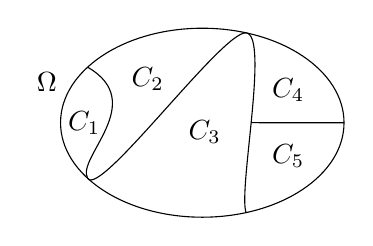
\begin{tikzpicture}[scale=.6]
				\draw (0,0) ellipse[x radius=3cm, y radius=2cm];
				\foreach \i in {1,...,5} \path ({360/5*\i}:3cm and 2cm) coordinate (A\i);
				\path (-2.5,0) node {$C_1$};
				\path (130:0.6*3cm and 0.6*2cm) node {$C_2$};
				\path (280:0.1*3cm and 0.1*2cm) node {$C_3$};
				\path (30:0.7*3cm and 0.7*2cm) node {$C_4$};
				\path (-30:0.7*3cm and 0.7*2cm) node {$C_5$};
				\draw[name path=curve]
				(A4)
				.. controls +(110:0.5) and +(-5:0.5) ..
				(A1)
				.. controls +(175:0.5) and +(-60:0.5) ..
				(A3)
				.. controls +(120:0.5) and +(-30:1.5) ..
				(A2);
				\path[name path=line] (0,0) -- (3,0);
				\path[name intersections={of=curve and line, by=Z}];
				\draw (Z) -- (3,0);
				\path (160:3cm and 2cm) coordinate (A);
				\path (A) ++(160:.5cm) node (omega) {$\Omega$};
			\end{tikzpicture}
		\end{columns}
		\vspace{5pt}
		{\bf\underline{The law of total probability}} \par
		If $\lbrace C_i\rbrace_{i=1}^n$ is a partition of $\Omega$, then:
		\begin{eqnarray*}
			P(A)&=&\sum_{i=1}^nP(A\cap C_i)\\
			&=&\sum_{i=1}^nP(A\vert C_i)P(C_i)
		\end{eqnarray*}
		{\small\color{NavyBlue} - we can derive this from the axioms of probability \par
			- this rule is very useful - especially wen stated in terms of conditional probability}
	\end{frame}

    \begin{frame}
    	\frametitle{Independence}
    	{\bf\underline{Definition}} \par
    	Events $A$ and $B$ are independent if information about $A$ does not effect uncertainty $B$ \par
    	Formally, $A$ and $B$ are independent if:
    	$$P(A\vert B)=P(A)$$
    	{\bf\underline{Exercise}} \par
    	Show that $P(A\vert B)=P(A)\Leftrightarrow P(B\vert A)=P(B)$ \par
    	%{\bf\underline{Question}} \par
        Note: $P(A\cap B)=P(A\vert B)P(B)$ so independence is equivalent to the statement:
        $$P(A\cap B)=P(A)P(B)$$
        A set of events $X_1,X_2,\dots,X_n$ are independent if: \par
        For all subsets $\{X_{i_1},X_{i_2},\dots,X_{i_k}\}$ of $\{X_1,X_2,\dots,X_n\}$, we have:
        %$$P(\cap_{j=1}^kX_{i_j})=\prod_{j=1}^kX_{i_j}$$
        $$P(X_{i_1}\cap X_{i_2}\cap\dots\cap X_{i_k})=P(X_{i_1})P(X_{i_2})\dots P(X_{i_k})$$
        \color{black}{
        %any pair are independent as above. \par
        %This gives:
        %$$P(\cap_{i=1}^n A_i)=\prod_{i=1}^nP(A_i)\quad\forall A_i\subseteq\Omega$$
        {\bf Question: what does independence look like on a Venn diagram?}
        }
    \end{frame}
	
	\begin{frame}
		\frametitle{What is probability?}
		{\bf\underline{Frequestist definition}} \par
		Probability is the long-run relative frequency of an event occurring when an experiment is repeated under identical conditions:
		$$P(A)=\lim_{n\rightarrow\infty}\frac{k_n(A)}n$$
		where $k_n(A)$ denotes the observed number of occurences of $A$ in $n$ trials \par
		{\small\color{NavyBlue} - here is objective and based on observed data: each event has a true, fixed parameter defining its probability \par
			- ther remainder of MATH163 will assume the frequentist interpretation of probability} \par
		{\bf\underline{Bayesian definition}} \par
		Probability represents a degree of belief or certainty about an event, updated as new evidence is observed. Recall:
		$$P(\theta\vert D)=\frac{P(D\vert\theta)P(\theta)}{P(D)}$$
		where $P(\theta\vert D)$ is the updated probability of a parameter $\theta$ given data $D$ \par
		{\small\color{NavyBlue} - you will still need to understand and use Bayes' rule in MATH163!}
	\end{frame}
	
	\begin{frame}
		\frametitle{$\bigstar$ Recap: rules of probability}
		Let $\Omega$ be an event space and $A,B\subseteq \Omega$ and let $\lbrace C_i\rbrace_{i=1}^n$ be partition of $\Omega$. Then:
		\begin{eqnarray}
			&&P(\overline A)=1-P(A)\\
			&&P(\emptyset)=0\\
			&&A\subseteq B\Rightarrow P(A)\leq P(B)\\
			&&P(A\cup B)=P(A)+P(B)-P(A\cap B)\\
			&&P(A)=\sum_{i=1}^nP(A\cap C_i)=\sum_{i=1}^nP(A\vert C_i)P(C_i)\\
			&&P(A\vert B)=\frac{P(B\vert A)P(A)}{P(B)}=\frac{P(B\vert A)P(A)}{P(B\vert A)P(A)+P(B\vert\overline A)P(\overline A)}
		\end{eqnarray}
		Note:
		\begin{itemize}
			\item $A$ and $B$ are mutually exclusive if $P(A\cap B)=0)$ \par
			$\Rightarrow P(A\cup B)=P(A)+P(B)$
			\item $A$ and $B$ are independent if $P(A\vert B)=P(A)$ \par
			$\Rightarrow P(A\cap B)=P(A)\times P(B)$ \par
			%{\small\color{NavyBlue} - we will explore this more in week 4}
		\end{itemize}
	\end{frame}
	
	\begin{frame}
		\frametitle{$\bigstar$ How to answer questions}
		%It's important to understand where he rules of probability come from \par
		It's easy to get in a tangle when answering exam questions about probability \par
		- just like it's easy to misinterpret probabilities in the real world \par
		Here is a step-by-step guide to approach a probability problem:
		\begin{enumerate}
			\item Label all events of interest, \par
			e.g. ``true +", ``true -", ``test +", ``test -" \par
			{\small\color{NavyBlue} - they need not be mutually exclusive or independent}
			\item Write down what you know in the language of probability, \par
			e.g. $P(test +\vert true\ -)=0.2$ \par
			{\small\color{NavyBlue} - be careful to get conditionality the right way round!}
			\item Write down what you want to know, e.g. $P(true +\vert test\ +)$
			\item Use only the rules of probability provided to calculate what you want to know using what you have been given, e.g. apply Bayes' rule
		\end{enumerate}
		{\small\color{NavyBlue} - this seems obvious, but it's REALLY easy to jump ahead and get in a tangle}
	\end{frame}
	
	\begin{frame}
		\frametitle{Probability: example 1}
        {\small
		\begin{enumerate}
            \item Labels: ``true +", ``true -", ``test +", ``test -"
			\item $0.015$ of the female population is estimated develop cancer per year: $P(true\ +)=0.00015$; \par
			$12m$ women underwent annual screening: $n=1.2\times 10^7$; \par
			the false positive rate is $20\%$: $P(test\ +\vert true\ -)=0.2$ \par
			the false negative rate was $5\%$: $P(test\ -\vert true\ +)=0.05$
            \item We want to know: $P(true\ +\vert test\ +)$
		%\end{enumerate}
        \item Apply the rules:
		%{\small
			\begin{eqnarray*}
				P(true\ +\vert test\ +)&=&\frac{P(test\ +\vert true\ +)P(true\ +)}{P(test\ +)}\quad\text{(Bayes' rule)}\\
				P(test\ +)&=&P(test\ +\vert true -)P(true\ -)+P(test\ +\vert true +)P(true\ +)\quad\text{(LTP)}\\
				%&=&0.2\times 0.015+0.8\times 0.985=0.209\\
				\text{so}\ P(true\ +\vert test\ +)&=&\frac{0.95\times 0.00015}{0.2\times 0.99985+0.95\times 0.00015}\\
				&\approx&0.00071
			\end{eqnarray*}
		%}
		- this is $0.071\%$! %\par
        \end{enumerate}
        }
		{\small\color{NavyBlue} - by the law of total probability, the denominator in Bayes' rule is a sum, and the numerator is one of the terms in the sum \par
			- we didn't need to use all of the information that was given in order to answer the question!} \par
		Question: what percentage of women who tested negative were true positives?
	\end{frame}
	
	\begin{frame}
		\frametitle{Probability: example 1}
		Why is this so confusing? \par
		{\bf Mistake:} \par
		``A $20\%$ false positive rate means if I test positive I'm $80\%$ likely to have the disease" \par
		{\bf Truth:} ``A $20\%$ false positive rate means that $20\%$ of the true negatives will test positive" \par
		{\small\color{NavyBlue} - the proportion of true negatives testing positive depends on the proportion of true positives in the population!} \par
		
		\tikzstyle{box}=[draw, minimum width=5em, 
		text centered, minimum height=2.5em, line width=1.5pt]%,drop shadow]
		\begin{center}
			\begin{tikzpicture}[node distance=0cm,outer sep = 0pt]
				\node (A) [box,text width=15em,text height=6em] {};%{true -, test -};
				\node (B) [box,below= of A.east,anchor=west,text width=6em,text height=6em,fill=red!30] {};%{true +, test -};
				\node (C) [box,below= of A.south,anchor=north,text width=15em,fill=NavyBlue!30] {};%{true -, test +};
				\node (D) [box,below= of B.south,anchor=north,text width=6em,fill=black!60] {};%{true +, test +};
				\node (1) [below= of A.north,anchor=south] {true -};
				\node (2) [below= of B.north,anchor=south] {true +};
				\node (3) [left= of A.west,anchor=east] {test -};
				\node (4) [left= of C.west,anchor=east] {test +};
			\end{tikzpicture}
		\end{center}
		
		{\bf Question:} what percentage of women who tested negative were true positives?
	\end{frame}

    \begin{frame}
    	\frametitle{Probability: example 2}
    	%{\bf\underline{Exercise}} \par
    	%Select $20$ people in the room. What is the probability that at least $2$ of them share a birthday? \par
        %Note: P(A)=1-P(not A), but successive trials are not independent
        You are dealt a poker hand ($5$ cards from one deck). What is the probability of drawing at least one king? \par
        \includegraphics[width=\textwidth]{cards.png} \par
        Note: this can be done without considering successive draws as random variables!
    \end{frame}

    \begin{frame}
    	\frametitle{Probability: example 3}
    	Traffic accidents are known to be influenced by weather conditions. Suppose the probability of a traffic accident occurring on a given day depends on whether the day is sunny or rainy. Assume that every day is either sunny or rainy, and that $70\%$ of days are sunny. Only $5\%$ of sunny days have traffic accidents, whereas $15\%$ of rainy days have them. \par
        You work for the emergency services in a room with no windows. You get a call reporting a traffic accident. \par
        (a) What is the probability that today is rainy? \par
        (b) You have not seen a weather forecast. What is the probability of an accident occurring tomorrow? \par 
        (c) What assumptions have been made in your calculations?
    \end{frame}
	
	%%%%%%%%%%%%%%%%%%%%%%%%%%%%%%%%%%%%%%%%%%%%%%%%%%%%%%%%%%%%%%%%
	%%%%%%%%%%%%%%%%%%%%%%%%%%%%%%%%%%%%%%%%%%%%%%%%%%%%%%%%%%%%%%%%
	%%%%%%%%%%%%%%%%%%%%%%%%%%%%%%%%%%%%%%%%%%%%%%%%%%%%%%%%%%%%%%%%
	%%%%%%%%%%%%%%%%%%%%%%%%%%%%%%%%%%%%%%%%%%%%%%%%%%%%%%%%%%%%%%%%
\section{Week 3: transforming random variables}

\begin{frame}
\frametitle{Recap: random variables}
A random variable describes the outcome of an experiment before it has been observed \par
The {\bf event space} $\Omega_X$ of a random variable $X$ is the set of possible outcomes \par
Random variables can be:
\begin{itemize}
    \item {\bf Discrete:} the outcome space is finite or countably infinite \par
    (typically $\Omega\subseteq\mathbb Z$)
    \item {\bf Continuous:} the outcome space is uncountably infinite \par
    (typically $\Omega=(a,b),\ (0,\infty)$ or $\mathbb R$)
\end{itemize}
A random variable if fully characterised by a set of outcomes and the corresponding probabilities \par
More formally a random variable is characterised by a probability space
\end{frame}

\begin{frame}
\frametitle{Recap: discrete case}
Discrete random variables are characterised by {\bf probability mass functions (PMFs)} \par
If $X$ is a discrete random variable with pmf $p_X(x)$ and event space $\Omega_X$ then:
\begin{eqnarray*}
   P(X=k)&=&f_X(k)\\
   \sum_{k\in\Omega_X}f_X(k)&=&1\\
   f_X(x)\geq 0 && \forall x\in\Omega_X
\end{eqnarray*}
Continuous random variables are characterised by {\bf probability density functions (PDFs)} \par
If $Y$ is a continuous random variable with pdf $p_Y(y)$ and event space $\Omega_Y$ then:
\begin{eqnarray*}
   P(Y\in(a,b))&=&\int_a^bf_Y(y)dy\\
   \int_{-\infty}^{\infty}f_Y(y)&=&1\\
   f_Y(y)\geq 0 && \forall y\in\Omega_Y
\end{eqnarray*}
- a single value of a PDF is not a probability (hence ``density" rather than ``mass")
\end{frame}

\begin{frame}
\frametitle{Recap: cumulative density}
{\bf Cumulative density functions (CDFs)} can be defined for all random variables \par
\begin{eqnarray*}
   F_X(x):&=&P(X\leq x)\\
   &=&\sum_{k\leq x}p_X(k)\\
   F_Y(y)&=&P(Y\leq y)\\
   &=&\int_{-\infty}^yf_Y(t)dt
\end{eqnarray*}
Useful results:
\begin{eqnarray*}
P(X=x)&=&\lim_{z\rightarrow x^+}F_X(z)-\lim_{z\rightarrow x^-}F_X(z)\\
P(y\in(a,b))&=&F_Y(b)-F_Y(a)\\
f_Y(y)&=&\frac d{dy}F_Y(y)\\
f_Y(y)\geq 0\forall y\in\mathbb R &\Leftrightarrow & F_Y(y)\ \text{is monotone increasing}
\end{eqnarray*}
Random variables can also be fully characterised by their CDF
\end{frame}

\begin{frame}
\frametitle{Recap: mean and variance}
{\bf\underline{Mean/expectation}}
\begin{eqnarray*}
   E[X]:&=&\sum_{x\in\Omega X}xp_X(x)\\
   E[Y]:&=&\int_{-\infty}^{\infty}yf_Y(y)dy\\
\end{eqnarray*}
{\bf\underline{Variance}}
\begin{eqnarray*}
   Var(X):&=&\sum_{x\in\Omega X}(x-E[X])^2p_X(x)\\
   &=&\sum_{x\in\Omega X}x^2p_X(x)-E[X]\\
   &=&E[X^2]-E[X]^2\\
   Var(Y):&=&\int_{-\infty}^{\infty}(y-E[Y])^2f_Y(y)dy\\
   &=&\int_{-\infty}^{\infty}y^2f_Y(y)dy-E[Y]^2\\
   &=&E[Y^2]-E[Y]^2
\end{eqnarray*}
{\small\color{NavyBlue} - there is a sneaky transformed random variable in here, which will become clear this week}
\end{frame}

\begin{frame}
\frametitle{Warnings}
Sometimes continuous random variables are described by ``nice" functions, but only on specific intervals \par
Example:
\begin{eqnarray*}
    f_X(x) = \left\{\begin{array}{lr}
			\frac 1c(x^3-7x^2+15x-7), & x\in(1,4)\\
			0, & \text{otherwise}
		\end{array}\right.
\end{eqnarray*}
\begin{columns}
		\column{0.5\textwidth}
		\centering
		\fbox{\includegraphics[width=\textwidth]{contEgW3a.png}}
		PMF
		\column{0.5\textwidth}
		\centering
		\fbox{\includegraphics[width=\textwidth]{contEgW3b.png}}
		CDF
	\end{columns}
\end{frame}

\begin{frame}
\frametitle{Warnings}
\color{gray}
Sometimes continuous random variables are described by ``nice" functions, but only on specific intervals \par
Example:
\begin{eqnarray*}
    f_X(x) = \left\{\begin{array}{lr}
			\frac 1c(x^3-7x^2+15x-7), & x\in(1,4)\\
			0, & \text{otherwise}
		\end{array}\right.
\end{eqnarray*}
\color{black}
Important observation:
\begin{eqnarray*}
    \int_{-\infty}^{\infty}f_X(x)&=&\frac 1c\int_1^4(x^3-7x^2+15x-7)dx=1\\
    &\neq&\frac 1c\int_{-\infty}^{\infty}(x^3-7x^2+15x-7)dx
\end{eqnarray*}
- be careful with the limits on the integral! \par
{\bf We will not always use $X$ for a discrete random variable and $Y$ for a continuous random variable - beware of context!}
\end{frame}

\begin{frame}
\frametitle{Functions}
Functions give a single output for each input:
\begin{eqnarray*}
    f:U&\rightarrow& V\\
    u\in U&\mapsto& v\in V
\end{eqnarray*}
Random variables have no input: they are specified by assigning probabilities to events \par
PMFs, PDFs and CDFs are functions of the \it{outcome} of a random variable \par
\end{frame}

\begin{frame}
\frametitle{Equality between random variables}
%What does it mean for $2$ random variables to be equal? \par
Let $X$ and $X'$ be $2$ random variables. \par
Equality between random variables can be established in $2$ different ways:
\begin{itemize}
    \item {\bf Equality in distribution:} $X\stackrel{d}{=}X'$ \par
    $X$ and $X'$ follow the same distribution, i.e. are defined by the same PMF/PDF/CDF \par
    Example: rolling a dice, and picking a card from $\{A\clubsuit,2\clubsuit,3\clubsuit,4\clubsuit,5\clubsuit,6\clubsuit\}$
    \item {\bf Equality of variables:} $X=X'$ \par
    The outcome of $X$ is equal to the outcome of $X'$ \par
    Example: you roll a dice, and whichever number you roll is the number of pounds you win. ``Dice outcome" and ``prize money" are equal
\end{itemize}

\end{frame}

\begin{frame}
\frametitle{Functions of random variables}
Let $X$ be a random variable with event space and let $G:\Omega_X\rightarrow\Omega_Y$ be a function \par
We can define a random variable $Y=G(X)$ such that outcome $x$ of $X$ is mapped to $y=G(x)$ \par
Given a PMF or PDF for $X$, we often want to know the corresponding PDF or PMF of $Y=G(X)$ \par
{\bf This is NOT the same as} $p_Y(y)=G(p_X(x))$ \par
%Counter example: $X$ represents rolling a fair dice, $Y=X^2$ \par
In the discrete case, deriving the PMF of $Y$ is ``simply a matter of bookkeeping" \par
$$P(Y=k)=\sum_{G(x)=k}p_X(x)$$
{\small\color{NavyBlue} - count the different outcomes of $X$ that map to $k$, and add up the corresponding probabilities \par
- we can do this because individual outcomes form a partition of $\Omega_X$} \par
Note: we use capital letters for random variables ($V,W,X,Y,Z$), and capital letters for functions of random variables ($F,G,H$) since a function of a random variable is itself a random variable. We will avoid $F$ since this is also used for CDFs
\end{frame}

\begin{frame}
\frametitle{Example 1}
Simple game: you pay $\$A$ to enter - this is called the ante \par
A dice is rolled once. If you roll $1,2$ or $4$, you lose your money \par
Roll a $4$ or $5$ and win $\$5$, roll a $6$ and win $\$50$ \par
{\bf\underline{Question}} \par
You run the casino - what should the value of $A$ be in order for the game to make a profit?
\end{frame}

\begin{frame}
\frametitle{Example 1}
{\bf\underline{Answer}} \par
Let $X$ be a random variable describing the outcome of rolling a dice: $\Omega_X=\{1,2,3,4,5,6\}$ \par
Let $Y$ be the ammout of money won (not including the ante): $\Omega_Y=\{0,5,50\}$ \par
We have $Y=G(X)$ where:
$$
		p_X(x) = \left\{\begin{array}{lr}
			\frac 16, & x=1,2,3,4,5,6\\
			0, & \text{otherwise}
		\end{array}\right.,\qquad
        G(x)=\left\{\begin{array}{lr}
			5, & x\in\{4,5\}\\
            50, & x=6\\
			0, & \text{otherwise}
		\end{array}\right.
$$
From this we can calculate:
$$
		p_Y(y) = \left\{\begin{array}{lr}
            \frac 16, & y=50\\
			\frac 13, & y=5\\
			\frac 12, & y=0\\
            0, & \text{otherwise}
		\end{array}\right.\quad
        \color{gray}{
        \text{Recall:}\ P(Y=k)=\sum_{G(x)=k}p_X(x)
        }
$$
{\bf Warning: do not confuse an outcome $0$ with an outcome occurring with probability $0$}
\end{frame}

\begin{frame}
\frametitle{Example 1}
{\bf\underline{Answer}} \par
But we're not done... \par
In order for the casino to turn a profit, we need $A>E[Y]$:
\begin{eqnarray*}
    E[Y]&=&\sum_yyp_Y(y)\\
    &=&\frac 16\times 50+\frac 13\times 5\\
    &=&10
\end{eqnarray*}
%{\small\color{NavyBlue} - summing over $x$, some $x$'s may lead to the same $y$} \par
So pick $A>10$ - what can we get away with?
\end{frame}

\begin{frame}
    \frametitle{Transforming discrete random variables: mean}
    If $Y=G(X)$ then:
    \begin{eqnarray*}
        E[Y]:&=&\sum_yyP(Y=y)\\
        &=&\sum_yy\sum_{G(X)=y}P(X=x)\\
        &=&\sum_xG(x)P(X=x)\\
        \text{OR}\quad E[Y]&=&\sum_xG(x)p_X(x)\quad\text{(notation change)}
    \end{eqnarray*}
{\small\color{NavyBlue} - for each $y$, sum over the $x$'s that map to Y, or simply sum over $x$} \par
{\bf\underline{Question}} \par
If $Y=G(X)$, can we say $E[Y]=G(E[X])$?
\end{frame}

\begin{frame}
	\frametitle{Transforming discrete random variables: mean}
    {\bf\underline{Answer}} \par
	If $Y=mX+c$ then we have:
	\begin{eqnarray*}
		E[Y]&=&\sum_x (mx+c)p_X(x)\\
		&=&m\sum_x xp_X(x)dx+c\sum_x p_X(x)\\
		&=&mE[X]+c
	\end{eqnarray*}
	- this is the {\bf linearity} property of the expectation \par
	Likewise, if $Y=mG(X)+c$ then:
	$$E[Y]=mE[G(X)]+c$$
    BUT, consider the case $Y=X^2$ - can you show that $E[Y]=E[X]$ is not guaranteed? \par
    Hint: $G(E[X])=E[X]^2$
\end{frame}

\begin{frame}
	\frametitle{Transforming discrete random variables: variance}
	If $Y=G(X)$ then:
	\begin{eqnarray*}
		Var[Y]:&=&\sum_y y^2p_Y(y)-E[Y]^2\\
		&=&\sum_x G(x)^2p_X(x)
	\end{eqnarray*}
    {\bf\underline{Question}} \par
    If $Y=G(X)$, can we say $Var[Y]=G(Var[X])$? \par
    What if $G(X)=mX+c$?
\end{frame}

\begin{frame}
	\frametitle{Transforming discrete random variables: variance}
	If $Y=mX+c$ then we have:
	\begin{eqnarray*}
		Var[Y]&=&\sum_x (mx+c)^2p_X(x)-E[mX+c]^2\\
		&=&\sum_x (m^2x^2+2mcx+c^2)p_X(x)-(mE[X]+c)^2\\
		&=&m^2\sum_x x^2p_X(x)+2mc\sum_x xp_X(x)+c^2\sum_x p_X(x)-(mE[X]+c)^2\\
            &=&m^2E[X^2]+2mcE[X]+c^2-m^2E[X]^2-2mcE[X]-c^2\\
            &=&m^2Var(X)
	\end{eqnarray*}
	Likewise, if $Y=mG(X)+c$ then:
	$$Var(Y)=m^2G(Var(X))$$
    {\bf\underline{Corollary}} \par
    Adding a constant to a random variable does not change its variance!
\end{frame}

\begin{comment}
\begin{frame}
	\frametitle{Example 2}
	%Sometimes we know $p_X(x)$ or $f_X(x)$ but we are interested in a different random variable $Y=G(X)$ \par
	{\bf\underline{Example}} \par 
	Let $X$ denote the number of defective items in a batch of 10 items. Each item is defective with probability $p$. \par 
	The manufacturer has a policy where they reject any batch with more than $2$ defective items. The random variable $Y$ represents whether a batch is accepted ($Y=1$) or rejected ($Y=0$). \par 
	What is $p_Y(y)$ in terms of $p$?
	\begin{center}
		\fbox{\includegraphics[width=.2\textwidth]{countdown.jpg}}
	\end{center}
\end{frame}
\end{comment}

\begin{frame}
	\frametitle{Example 2}
    Let $X$ b a random variable representing the magnitude of an earthquake on the Richter scale in a specific region. We know:
    $$P(X=3)=0.2,\ P(X=4)=0.3,\ P(X=5)=0.3,\ P(X=6)=0.2,\ $$
    Let $Y$ denote the economic cost of an earthquake based on its magnitude:
    $$Y=G(X)=\frac {L}{1+e^{-k(X-X_0)}}$$
    Where:
    \begin{itemize}
        \item $L=10,000$ is the maximum possible damage in $\$millions$
        \item $X_0=5$ is the magnitude at which damage reaches half of the maximum
        \item $k=1.5$ controls the steepness of the curve
    \end{itemize}
    Note: all of this question is conditional on the event of an earthquake
\end{frame}

\begin{frame}
	\frametitle{Example 2}
    {\bf\underline{Exercise}} \par
    \begin{itemize}
        \item Compute $E[X]$ and $Var(X)$
        \item Write down the PMF of $Y$
        \item Compute $E[Y]$ and $Var(Y)$
        \item The energy released in an earthquake is modeled as $E=E_0\times 10^{1.5X}$, where $E_0$ is the reference energy (magnitude $0$). Explain why we do not use an exponential transformation to model economic cost
    \end{itemize}
    \begin{center}
		\fbox{\includegraphics[width=.2\textwidth]{countdown.jpg}}
	\end{center}
    Hint: sketch the function $y=G(x)$ as a continuous curve first, even though $X$ is discrete
\end{frame}

\begin{frame}
\frametitle{Example 3: Lotto}
Disclaimer: this example brings together combinatorics, probability and transformed random variables. It is more involved than any single assessment question \par
The rules of lotto:
\begin{itemize}
    \item A single ticket costs $\pounds 2$
    \item You pick $6$ distinct numbers between $1$ and $59$
    \item $6$ main balls are drawn from a set numbered $1-59$, plus one bonus ball (BB)
    \item You win money if your numbers match the balls, with prizes as follows:
    \begin{table}
    \centering
    \begin{tabular}{|l|l|}
    \hline 
    Match & Prize \\ \hline
    Exactly $3$ main balls & $\pounds 30$ \\
    Exactly $4$ main balls & $\pounds 140$ \\
    Exactly $5$ main balls and NOT the BB & $\pounds 1,750$ \\
    Exactly $5$ main balls + BB & $\pounds 1,000,000$ \\
    All $6$ main balls & Jackpot $\pounds J$ \\ \hline
    \end{tabular}
    \end{table}
\end{itemize}
\end{frame}

\begin{frame}
\frametitle{Example 3: Lotto}
{\bf\underline{Questions}} \par
\begin{itemize}
    \item What is the expected win on a single lottery ticket (in terms of $J$)?
    \item How much would the jackpot have to be in order for the lottery to be on lucrative for players in the long run?
    \item $N$ tickets are sold. Write an equation describing the expected gross profit made from the lottery in terms of $N$ and $J$
\end{itemize}
\end{frame}

\begin{frame}
\frametitle{Example 3: Lotto}
We $^*$could$^*$ fix out ticket numbers and view the lottery draw as the random variable \par
Equivalently, we could fix the draw numbers and view our ticket selection as a random variable
\begin{itemize}
    \item If $X$ represents your number selection, then $\Omega_X$ is the set of all subsets of $\{1,2,\dots,59\}$ that contain exactly $6$ elements
    %\item $X$ is discrete uniform (if the lottery machine is fair!)
    \item $X$ follows a discrete uniform distribution
    \item Let $Y=G(X)$ denote the prize for line $X$
    \item A lottery line is a set of numbers. Order does not matter - it is therefore common practice list numbers in numerical order
\end{itemize}
\end{frame}

\begin{frame}
\frametitle{Example 3: Lotto}
Start by asking: how many ways are there for my ticket to match the lottery draw in each winning category
\begin{table}
\centering
\begin{tabular}{|l|c|c|}
    \hline 
    Match & Calculation & Value \\ \hline
    $3$ main & ${{6}\choose{3}}\times{{53}\choose{3}}$ & $468,520$ \\
    $4$ main & ${{6}\choose{4}}\times{{53}\choose{2}}$ & $20,670$ \\
    $5$ main, not BB & ${{6}\choose{5}}\times{{53}\choose{1}}\times\frac{52}{53}$ & $312$ \\
    $5$ main + BB & ${{6}\choose{5}}\times{{53}\choose{1}}\times\frac{1}{53}$ & $6$ \\
    All $6$ main balls & ${6\choose 6}$ & $1$ \\ \hline
    \end{tabular}
    \end{table}
(note that ${{53}\choose{52}}={{53}\choose{1}}=\frac 1{53}$) \par
Now ask: how many distinct ticket possibilities are there?
$${59\choose 6}=45,057,474$$
\end{frame}

\begin{frame}
\frametitle{Example 3: Lotto}
Putting it all together:
\begin{table}
\centering
\begin{tabular}{|l|c|c|}
    \hline 
    Event ($A\subseteq\Omega_X$) & Combinations ($|A|$) & Prize ($Y$) \\ \hline
    $3$ main & $468,520$ & $30$\\
    $4$ main & $20,670$ & $140$\\
    $5$ main, not BB & $312$ & $1,750$\\
    $5$ main + BB & $6$ & $1,000,000$\\
    All $6$ main balls & $1$ & $J$ \\ \hline
    \end{tabular}
    \end{table}
    and $|\Omega_X|=45,057,474$ \par
Let $A_y\subseteq\Omega_X$ the set $\{x\in X|G(x)=y\}$. Then:
\begin{eqnarray*}
    P(Y=y)\sum_y\frac{|A_y|}{|\Omega_X|}\qquad\text{and}\qquad E[Y]&=&\sum_yyP(Y=y)\\
    &=&\frac 1{|\Omega_X|}\sum_y|A_y|\\
    &=&\frac J{45,057,474}+\dots
\end{eqnarray*}
\end{frame}

\begin{frame}
\frametitle{Example 3: Lotto}
{\bf\underline{Answers}} \par
\begin{itemize}
    \item What is the expected win on a single lottery ticket (in terms of $J$)?
    \color{red}
    $$\mathbf{E[Y]=\pounds\left(\frac J{45,057,474}+0.521454\right)}$$
    \color{black}
    \item How much would the jackpot have to be in order for the lottery to be lucrative for players?
    \color{red}
    $$\frac J{45,057,474}+0.521454>2\Rightarrow J>\frac{2-0.521454}{45,057,474}=\mathbf{\pounds 66,619,548}$$
    \color{black}
    \item $N$ tickets are sold. Write an equation describing the expected gross profit made from the lottery in terms of $N$ and $J$
    \color{red}
    $$profit=2N-N\times E[Y]=\mathbf{\pounds N\left(1.478546-\frac J{45,057,474}\right)}$$
    \color{black}
    - this actually uses a bit of assumed knowledge from the week 4 material \par
    (expectation of a sum of random variables)
\end{itemize}
\end{frame}

\begin{comment}
\begin{frame}
\frametitle{Fun example}
The St. Petersburg lottery is played as follows:
\begin{itemize}
    \item A player pays an ante of $\$A$ to enter
    \item Round $1$: $\$2$ prize is placed down and a coin is tossed \par
    HEADS you take the prize money, TAILS you continue to round $2$
    \item Round $2$: the prize money is doubled and a coin is tossed \par
    HEADS you take the prize money, TAILS you continue to round $3$ 
    \item Round $i$: the prize money is doubled and a coin is tossed \par
    HEADS you take the prize money, TAILS you continue to round $i+1$
\end{itemize}
{\bf\underline{Questions}}
\begin{enumerate}
    \item What is the expected amount of money won?
    \item If you ran the casino, what would you charge as the ante?
\end{enumerate}
\end{frame}

\begin{frame}
\frametitle{Fun example}
{\bf\underline{Answers}} \par
The key is to define random variables: \par
Let $X$ be the number of rounds played and $Y$ be the total won - then $Y=2^Y$ \par
The game stops at round $i$ if $i-1$ tails are tossed in a row, followed by $1$ head \par
There is only one way for this to happen, and each toss happens independently, so: $$P(X=i)=\left(\frac 12\right)^2$$
%$i\mapsto 2^i$ is $1-1$ and so we have:
%$$P(Y=2^i)=\left(\frac 12\right)^2$$
Crucially, we can calculate:
$$E[Y]=\sum_{i=1}^{\infty}2^i\frac 1{2^i}$$
...which diverges!
Note, however:
$$E[X]=\sum_{i=1}^{\infty}\frac i{2^i}$$
And this sum converges to $2$ (proof omitted) \par
{\bf We will revisit this example when studying the geometric distribution} \par
- homework: revise the geometric series
%Here, we have $X=Y$ - the strongest equality between random variables! \par
%{\bf This answer is beyond the scope of assessment in MATH163 as it includes some theory from other courses}
\end{frame}
\end{comment}

\begin{frame}
	\frametitle{Transforming random variables}
	But what if $X$ is a continuous random variable? \par
	{\bf\underline{Example 4}} \par 
	We observe time taken to drive $1km$ on a motorway is (approximately) uniformly distributed between $40$ and $60$ seconds. \par
    We have $T\sim Unif(40,60),\ X=\frac 1T$ \par 
	What is the distribution of average speed $X$?
	%The trick: think in terms of CDFs
\end{frame}

\begin{frame}[t]
	\frametitle{$\bigstar$ Transforming random variables}
	{\small
		\begin{minipage}{\textwidth}
			\begin{columns}[T]
				\column{0.17\textwidth}
				\column{0.35\textwidth}
				\underline{General case} \par
				$Z=G(X),\ f_X(x)$ known
				\column{0.4\textwidth}
				\underline{Example 5} \par
				$Z=X^2+1,\ f_X(x)=e^{-x},\ x\geq 0$
			\end{columns}
		\end{minipage} \par
		\begin{minipage}{\textwidth}
			\begin{columns}[T]
				\column{0.17\textwidth}
				\underline{Step 1} \par
				Compute CDF of $X$
				\column{0.35\textwidth}
				\hfill \break \hfill \break
				$F_X(x)=P(X\leq x)$
				\column{0.4\textwidth}
				\hfill \break \hfill \break
				$F_X(x)=\int_0^xe^{-t}dt$ \par
				$\qquad\quad\ =1-e^{-x}$
			\end{columns}
		\end{minipage} \par
		\begin{minipage}{\textwidth}
			\begin{columns}[T]
				\column{0.17\textwidth}
				\underline{Step 2} \par
				Write $F_Z(z)$ in terms of $X$
				\column{0.35\textwidth}
				\hfill \break \hfill \break
				$P(Z\leq z)=P(G(X)\leq z)$
				\column{0.4\textwidth}
				\hfill \break \hfill \break
				$P(Z\leq z)=P(X^2+1\leq z)$
			\end{columns}
		\end{minipage} \par
		\begin{minipage}{\textwidth}
			\begin{columns}[T]
				\column{0.17\textwidth}
				\underline{Step 3} \par
				Rearrange the inequality in terms of $X$
				\column{0.35\textwidth}
				\hfill \break \hfill \break
				$P(Z\leq z)=P(X\leq G^{-1}(z))$
				\column{0.4\textwidth}
				\hfill \break \hfill \break
				$P(Z\leq z)=P(X\leq \sqrt{z-1})$
			\end{columns}
		\end{minipage} \par
		\begin{minipage}{\textwidth}
			\begin{columns}[T]
				\column{0.17\textwidth}
				\underline{Step 4} \par
				Substitute CDF of $X$
				\column{0.35\textwidth}
				\hfill \break \hfill \break
				$F_Z(z)=F_X(G^{-1}(z))$
				\column{0.4\textwidth}
				\hfill \break \hfill \break
				$P(Z\leq z)= 1-e^{-\sqrt{z-1}}$
			\end{columns}
		\end{minipage} \par
		\begin{minipage}{\textwidth}
			\begin{columns}[T]
				\column{0.17\textwidth}
				\underline{Step 5} \par
				Differentiate w.r.t. $z$
				\column{0.35\textwidth}
				\hfill \break \hfill \break
				$f_Z(z)=\frac d{dx}F_Z(z))$ \par
				$\qquad\ \ =\frac d{dx}F_X(G^{-1}(z))$
				\column{0.4\textwidth}
				\hfill \break \hfill \break
				$f_Z(z)=\frac d{dx}(1-e^{-\sqrt{z-1}})$ \par
				$\qquad\ \ =\frac 1{2\sqrt{z-1}}e^{-\sqrt{z-1}},\ z>1$ \par
				\color{NavyBlue}{{\tiny - please do check this!}}
			\end{columns}
		\end{minipage} \par
		%\begin{itemize}
	%		\item Warning: upper case denotes random variables and lower case specific values \par
	%		\item Questions: why does this trick work? What are its limitations?
	%		%Answer: CDF monotone increasing, ...
	%	\end{itemize}	
	}
    Warning: upper case denotes random variables and lower case specific values
\end{frame}

\begin{frame}
	\frametitle{Example 6}
	{\bf\underline{Exercise}} \par
	A continuous random variable $X$ is uniformly distributed on the interval $(0,\frac{\pi}2)$ \par
    Let $Y=\sin(X)$
    \begin{itemize}
        \item Find the PDF of $Y$
        \item Sketch the PDFs of $X$ and $Y$
    \end{itemize}
    \begin{center}
		\fbox{\includegraphics[width=.2\textwidth]{countdown.jpg}}
	\end{center}
    Hint: you may need to look up a bit of calculus \par
    This question is here to show you that the answer may not be what you expect \par
\end{frame}

\begin{frame}
	\frametitle{Transforming random variables}
	Recall the traffic example (example 4): $T\sim Unif(40,60),\ X=\frac 1T$ \par
	{\bf\underline{Questions}} \par
    \begin{itemize}
        \item What is the PDF of $X$?
        \item What are the limitations of this method?
    \end{itemize}
\end{frame}

\begin{frame}
	\frametitle{Transforming random variables}
	{\bf\underline{Answers}} \par
	\begin{enumerate}
		\item $F_T(t)=\frac 1{20}(t-40),\ t\in[40,60]$
		\item $F_X(x)=P(\frac 1T\leq x)$
		\item $F_X(x)=P(T\geq \frac 1x)=1-P(T\leq\frac 1x),\ x\in[\frac 1{60},\frac 1{40}]$
		\item $F_X(x) =1-\frac 1{20}(\frac 1x-40)=3-\frac 1{20}x^{-1}$
		\item $f_X(x)=\frac d{dx}[3-\frac 1{20}x^{-1}]=\frac 1{20x^2}$
	\end{enumerate}
	Limitation: we need $G(T)$ to be 1-1 so that $G^{-1}$ is well defined
\end{frame}

\begin{comment}
\begin{frame}
	\frametitle{Transforming random variables: mean}
	If $Y=G(X)$, then what is $E[Y]$? \par
	Be careful: we can not always say $E[Y]=G(E[X])$ \par
        Counter example: $Y=X^2$ \par
        Here, $E[X^2]=Var(X)+E[X]^2$, so $E[X^2]=E[X]^2$ only if $Var(X)=0$ \par
        {\bf This applies to both the discrete and continuous case!} \par
        
\end{frame}
\end{comment}

\begin{frame}
	\frametitle{Transforming continuous random variables: mean}
	If $Y=mX+c$ then we have:
	\begin{eqnarray*}
		E[Y]&=&\int (mx+c)f_X(x)dx\\
		&=&m\int xf_X(x)dx+c\int f_X(x)dx\\
		&=&mE[X]+c
	\end{eqnarray*}
	- this is the {\bf linearity} property of the expectation \par
	Likewise, if $Y=mG(X)+c$ then:
	$$E[Y]=mE[G(X)]+c$$
    {\bf This is exactly the same result as for the discrete case!}
\end{frame}

\begin{frame}
	\frametitle{Transforming continuous random variables: variance}
	If $Y=G(X)$, then: \par
	\begin{eqnarray*}
		Var[Y]:&=&\int y^2f_Y(y)dy-E[Y]^2\\
		&=&\int G(x)^2f_X(x)dx
	\end{eqnarray*}
	If $Y=mX+c$ then we have:
	\begin{eqnarray*}
		Var[Y]&=&\int (mx+c)^2f_X(x)dx-E[mX+c]^2\\
		&=&\int (m^2x^2+2mcx+c^2)f_X(x)dx-(mE[X]+c)^2\\
		&=&m^2\int x^2dx+2mc\int xf(x)dx+c^2\int f_X(x)dx-(mE[X]+c)^2\\
            &=&m^2E[X^2]+2mcE[X]+c^2-m^2E[X]^2-2mcE[X]-c^2\\
            &=&m^2Var(X)
	\end{eqnarray*}
	Likewise, if $Y=mG(X)+c$ then:
	$$E[Y]=mE[G(X)]+c$$
    {\bf This is exactly the same result as for the discrete case!}
\end{frame}

\section{Week 4: combining random variables}
%Limit laws

\begin{comment}
\begin{frame}
	\frametitle{Probability: important observations}
    In weeek 2 we talked about the probability of events $A,B$ etc. \par
    Otherwise, we have talked abour random variables $X,Y$ etc. \par
    What is the difference between an event and a random variable?
	\begin{itemize}
		\item $P(A)=P(x\in A)=\sum_{a\in A}P(X=a)$ (discrete case)
		\item $P(A)=P(x\in A)=\int_Af_X(a)da$ (continuous case)
	\end{itemize}
    {\bf Events are subsets of an event space, probabilities are sums/integrals of a PMF/PDF over that subset} \par
    Also note:
    \begin{itemize}
		\item $P(X=a)=lim_{a\rightarrow x^+}F_X(x)-lim_{a\rightarrow x^-}F_X(x)$ (discrete case)
		\item $f_X(x)=\frac d{dx}F_X(x)$ (continuous case)
    \end{itemize}
    {\bf Knowing the PMF/PDF OR CDF of a random variable completely characterizes its distribution} \par
        {\small\color{NavyBlue} - the PMF/PDF can be derived exactly from the CDF (probability is to a pdf what mass is to density, or what displacement is to velocity) \par
        - when integrating $f_X(X)$ to get $F_X(X)$, the constant of integration is fully determined by the law of total probability!}
    
\end{frame}
\end{comment}

\begin{frame}
    \frametitle{Recap}
    One random variable van be a function of another, i.e. $Y=G(X)$ \par
    Here, we apply the function $G$ to the outcome of the random variable $X$ \par
    Classic example: outcomes from a randomised process (lottery machine) are mapped to payouts (lottery winning) \par
    This is {\bf different} to the idea of combining distinct random variables, e.g. $Z=X+Y$ \par
    In reality, we apply functions to sums of variables, or sum functions of variables \par
    MATH163 will introduce this idea in simple terms
\end{frame}

\begin{frame}
	\frametitle{Combining random variables}
        In the casino game ``craps", players roll $2$ dice \par
        If $X_1$ and $X_2$ are the outcomes from rolling each dice, then $Y=X_1+X_2$ is a new random variable \par
        What is the PMF of $Y$? \par
        \begin{center}
    \renewcommand{\arraystretch}{1.5}
    \setlength{\tabcolsep}{10pt}
    \begin{tabular}{c c|c|c|c|c|c|c|}
        ~ & \multicolumn{7}{c}{Outcome of $X_1$} \\
        %\hline
        %\rowcolor[HTML]{C0C0C0}
        & \textbf{} & \textbf{1} & \textbf{2} & \textbf{3} & \textbf{4} & \textbf{5} & \textbf{6} \\%Die 1 / Die 2
        \cline{2-8}
        \multirow{6}{*}{\rotatebox[origin=c]{90}{\parbox[c]{2cm}{\centering Outcome of $X_2$}}} & \textbf{1} & \cellcolor[HTML]{FFC7C7}2  & \cellcolor[HTML]{FFDDC7}3 & \cellcolor[HTML]{FFEFC7}4 & \cellcolor[HTML]{F7FFC7}5 & \cellcolor[HTML]{D2FFC7}6 & \cellcolor[HTML]{C7FFF2}7 \\
        \cline{2-8}
        & \textbf{2} & \cellcolor[HTML]{FFDDC7}3  & \cellcolor[HTML]{FFEFC7}4 & \cellcolor[HTML]{F7FFC7}5 & \cellcolor[HTML]{D2FFC7}6 & \cellcolor[HTML]{C7FFF2}7 & \cellcolor[HTML]{C7E7FF}8 \\
        \cline{2-8}
        & \textbf{3} & \cellcolor[HTML]{FFEFC7}4  & \cellcolor[HTML]{F7FFC7}5 & \cellcolor[HTML]{D2FFC7}6 & \cellcolor[HTML]{C7FFF2}7 & \cellcolor[HTML]{C7E7FF}8 & \cellcolor[HTML]{C7C7FF}9 \\
        \cline{2-8}
        & \textbf{4} & \cellcolor[HTML]{F7FFC7}5  & \cellcolor[HTML]{D2FFC7}6 & \cellcolor[HTML]{C7FFF2}7 & \cellcolor[HTML]{C7E7FF}8 & \cellcolor[HTML]{C7C7FF}9 & \cellcolor[HTML]{E7C7FF}10 \\
        \cline{2-8}
        & \textbf{5} & \cellcolor[HTML]{D2FFC7}6  & \cellcolor[HTML]{C7FFF2}7 & \cellcolor[HTML]{C7E7FF}8 & \cellcolor[HTML]{C7C7FF}9 & \cellcolor[HTML]{E7C7FF}10 & \cellcolor[HTML]{FFC7FF}11 \\
        \cline{2-8}
        & \textbf{6} & \cellcolor[HTML]{C7FFF2}7  & \cellcolor[HTML]{C7E7FF}8 & \cellcolor[HTML]{C7C7FF}9 & \cellcolor[HTML]{E7C7FF}10 & \cellcolor[HTML]{FFC7FF}11 & \cellcolor[HTML]{FFC7C7}12 \\
        \cline{2-8}
    \end{tabular}
\end{center}
\end{frame}

\begin{frame}
    \frametitle{Combining random variables: mean}
    Again with discrete variables, deriving the PMF for a sum is a matter of ``bookkeeping":
    %\vspace{5pt}
    \begin{columns}[b]
    \column{0.6\textwidth}
    \begin{table}
    \centering
    \begin{tabular}{|c|l c|}
    y & \multicolumn{2}{c|}{$P(Y=y)$} \\ \hline
    2 & $1/36$ & $\approx 0.0278$ \\ \hline
    3 & $2/36=1/18$ & $\approx 0.0556$ \\ \hline
    4 & $3/36=1/12$ & $\approx 0.0833$ \\ \hline
    5 & $4/36=1/9$ & $\approx 0.1111$ \\ \hline
    6 & $5/36$ & $\approx 0.1389$ \\ \hline
    7 & $6/36=1/6$ & $\approx 0.1667$ \\ \hline
    8 & $5/36$ & $\approx 0.1389$ \\ \hline
    9 & $4/36=1/9$ & $\approx 0.1111$ \\ \hline
    10 & $3/36=1/12$ & $\approx 0.0833$ \\ \hline
    11 & $2/36=1/18$ & $\approx 0.0556$ \\ \hline
    12 & $1/36$ & $\approx 0.0278$ \\ \hline
    \end{tabular}
    %\caption{Outcomes and Probabilities of Rolling Two Dice}
    %\label{tab:dice_probabilities}
    \end{table}
    \column{0.4\textwidth}
    \vspace{5pt}
    \fbox{\includegraphics[width=\textwidth]{Catan.jpg}}
    \centering
    What is a fair placement of scores on a Catan board?
    \end{columns}
\end{frame}

\begin{comment}
\begin{frame}
    \frametitle{Independence}
    {\bf\underline{Definition}} \par
    Random $X$ and $Y$ are independent if the outcome of one not effect the PMF/PDF of the other, i.e.
    $$P(X\in A,Y\in B)=P(X\in A)P(Y\in B)$$
    $\forall A\subseteq\Omega_X,B\subseteq\Omega_Y$ \par
    {\bf\underline{Theorem}} (not proved in MATH163) \par
    
    If $2$ random variables $X$ and $Y$ are independent, then:
    \begin{eqnarray*}
    %p_{X,Y}(x,y)&=&p_X(x)p_Y(y)\quad\text{(discrete case)}\\
    %f_{X,Y}(x,y)&=&f_X(x)f_Y(y)\quad\text{(continuous case)}\\
    %\text{and}\quad E[XY]&=&E[X]E[Y]
    E[XY]&=&E[X]E[Y]
    \end{eqnarray*}
    {\small\color{NavyBlue} - the proof is not hard but requires theory of joint distributions and multivariate calculus} \par
    Note: $E[X+Y]=E[X]+E[Y]$ always, but $E[XY]=E[X]E[Y]$ requires independence 
\end{frame}
\end{comment}

\begin{frame}
    \frametitle{Combining random variables: mean}
    {\bf\underline{Theorem}} (not proved in MATH163) \par
    If $X_1,X_2,\dots,X_n$ are random variables with $E[X_i]<\infty\ \forall i$ and $c,m_1,m_2,\dots,m_n\in\mathbb R$ then:
    \begin{eqnarray*}
        E\left[c+\sum_{i=1}^nm_iX_i\right]=c+\sum_{i=1}^nm_iE[X_i]
    \end{eqnarray*}
    More strongly, if $G_1,G_2,\dots,G_n$ are functions then:
    \begin{eqnarray*}
        E\left[c+\sum_{i=1}^nm_iG_i(X_i)\right]=c+\sum_{i=1}^nm_iE[G(X_i)]
    \end{eqnarray*}
    {\small\color{NavyBlue} - the proof here requires something beyond MATH163, though these results are quite intuitive} \par
    Question: what about variance?
    \begin{eqnarray*}
        Var\left(c+\sum_{i=1}^nm_iX_i\right)=?
    \end{eqnarray*}
\end{frame}

\begin{frame}%Note: used part of this in week 2
	\frametitle{Recap: independence}
	{\bf\underline{Definition}} \par
	Events $A$ and $B$ are independent if information about one does not effect uncertainty in the other \par
	Formally, $A$ and $B$ are independent if:
	$$P(A\vert B)=P(A)$$
	We know:
        \begin{eqnarray*}
            P(A\vert B)=P(A)&\Leftrightarrow&P(B\vert A)=P(B)\\
            &\Leftrightarrow&P(A\cap B)=P(A)P(B)
        \end{eqnarray*}
\end{frame}

\begin{frame}
    \frametitle{Independence}
    Important distinction: independence of events is not the same as independence of random variables \par
    Example: %$X$: pick a card; $Y$: pick another (without replacement); $A$: the first card is red; $B$: the second card is a queen 
    \begin{itemize}
        \item $X$: pick a card; $Y$: pick another (without replacement)
        \item $A$: the first card is red; $B$: the second card is a queen
    \end{itemize}
    Are $X$ and $Y$ independent? \par
    Are $A$ and $B$ independent? \par
    {\bf\underline{Definition}} \par
    Random $X$ and $Y$ are independent if the outcome of one not effect the PMF/PDF of the other, i.e.
    $$P(X\in A,Y\in B)=P(X\in A)P(Y\in B)$$
    $\forall A\subseteq\Omega_X,B\subseteq\Omega_Y$
\end{frame}

\begin{frame}
	\frametitle{Independence}
	In which of the following cases are the random variables $X$ and $Y$ independent?
	\begin{enumerate}
		\item $X$: roll a dice; $Y$: roll another dice
		\item $X$: Draw a card from a deck; $Y$: draw another
		\item $X$: LFC football score on Saturday; $Y$: LFC score the following week
		\item $X$: delay on the the 14:52 to Newcastle; $Y$: delay on the 15:52
		\item $X$: my flu test result; $Y$: Beyonce's flu test result
		\item $X$: my flu test result; $Y$: Daniel Colquitt's flu test result
	\end{enumerate}
\end{frame}

\begin{frame}
	\frametitle{Independence: key result}
    {\bf\underline{Theorem} (not proved in MATH163)} \par
    If $X_1,X_2,\dots,X_n$ are independent random variables then for any functions $G_1,G_2,\dots G_n$ we have:
    $$E[X_1\cdot X_2\cdots X_n]=E[X_1]\cdot E[X_2]\cdots E[X_n]$$
    More generally:
    $$E[G_1(X_1)\cdot G_2(X_2)\cdots G_n(X_n)]=E[G_1(X_1)]\cdot E[G_2(X_2)]\cdots E[G_n(X_n)]$$
    - independence is a very useful property!
\end{frame}

\begin{frame}
	\frametitle{Combining random variables: variance}
    {\bf\underline{Theorem}} \par
    If $X_1,X_2,\dots,X_n$ are {\bf independent} random variables with $Var(X_i)<\infty\ \forall i$ and $c,m_1,m_2,\dots,m_n\in\mathbb R$ then:
    \begin{eqnarray*}
        Var\left(c+\sum_{i=1}^nm_iX_i\right)=\sum_{i=1}^nm_i^2Var(X_i)
    \end{eqnarray*}
    We can only sum variances when the random variables are {\bf independent} - why? \par
\end{frame}

\begin{frame}
	\frametitle{Combining random variables: variance}
    {\bf\underline{Proof}} \par
    For simplicity of notation we prove for the case of $X+Y$. Extending this to the general case is trivial. \par
    For any random variables $X$ and $Y$ with $Var(X),Var(Y)<\infty$, we have:
    \begin{eqnarray*}
        Var(X+Y)&=&E[(X+Y)^2]-E[X+Y]^2\\
        &=&E[X^2+2XY+Y^2]-\left(E[X]+E[Y]\right)^2\\
        &=&E[X^2]+2E[XY]+E[Y^2]-E[X]^2-2E[X]E[Y]-E[Y]^2\\
        &=&Var(X)+Var(Y)+2\left(E[XY]-E[X]E[Y]\right)\\
        %&=&Var(X)+Var(Y)\quad\text{iff}\ E[XY]-E[X]E[Y]
    \end{eqnarray*}
    %$E[XY]=E[X]E[Y]$ is an equivalent definition of independence (c.f. previous slide), which gives
    $Var(X+Y)=Var(X)+Var(Y)$ if $X$ and $Y$ are independent (c.f. previous slide) \par
    Note: it is possible to have $E[XY]=E[X]E[Y]$ in $2$ dependent variables, e.g. $X$ symmetric and $Y=X^2$
\end{frame}

\begin{frame}
	\frametitle{Covariance}
    {\bf\underline{Definition}} \par
    The {\bf covariance} of $2$ random variables $X$ and $Y$ is given by:
    \begin{eqnarray*}
        Cov(X,Y):&=&E\left[(X-E[X])(Y-E[Y])\right]\\
        &=&E\left[XY-XE[Y]-YE[X]+E[X]E[Y]\right]\\
        &=&E[XY]-E[X]E[Y]-E[Y]E[X]+E[X]E[Y]\\
        &=&E[XY]-E[X]E[Y]\\
    \end{eqnarray*}
    %{\small\color{NavyBlue} - note that if $X=Y$, this is just the variance of $X$} \par
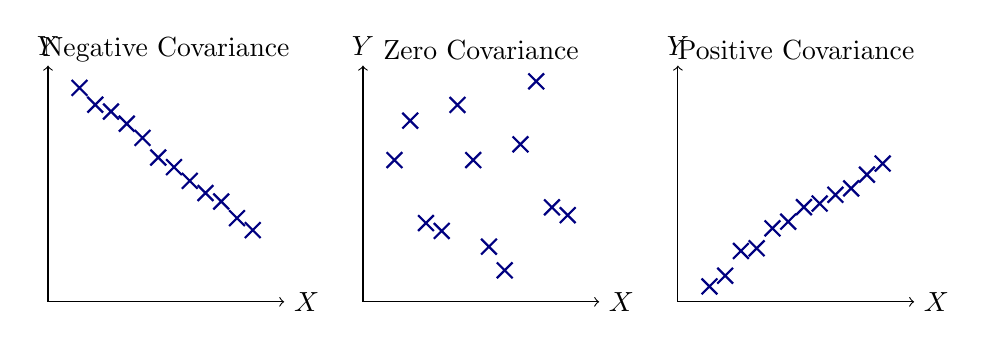
\begin{tikzpicture}

% Negative Covariance Plot
\begin{scope}[shift={(0,0)}]
    \node at (1.5, 3.2) {Negative Covariance};
    \draw[->] (0,0) -- (3,0) node[right] {$X$};
    \draw[->] (0,0) -- (0,3) node[above] {$Y$};
    \foreach \x in {0.4, 0.8, 1.2, 1.6, 2, 2.4, 0.6, 1, 1.4, 1.8, 2.2, 2.6}
        \draw[NavyBlue, thick] (\x, {3-0.8*\x-rand/15}) +(-0.1,-0.1) -- +(0.1,0.1) +(-0.1,0.1) -- +(0.1,-0.1);
\end{scope}

% Zero Covariance Plot
\begin{scope}[shift={(4,0)}]
    \node at (1.5, 3.2) {Zero Covariance};
    \draw[->] (0,0) -- (3,0) node[right] {$X$};
    \draw[->] (0,0) -- (0,3) node[above] {$Y$};
    \foreach \x/\y in {0.4/1.8, 0.8/1, 1.2/2.5, 1.6/0.7, 2/2, 2.4/1.2, 0.6/2.3, 1/0.9, 1.4/1.8, 1.8/0.4, 2.2/2.8, 2.6/1.1}
        \draw[NavyBlue, thick] (\x, \y) +(-0.1,-0.1) -- +(0.1,0.1) +(-0.1,0.1) -- +(0.1,-0.1);
\end{scope}

% Positive Covariance Plot
\begin{scope}[shift={(8,0)}]
    \node at (1.5, 3.2) {Positive Covariance};
    \draw[->] (0,0) -- (3,0) node[right] {$X$};
    \draw[->] (0,0) -- (0,3) node[above] {$Y$};
    \foreach \x in {0.4, 0.8, 1.2, 1.6, 2, 2.4, 0.6, 1, 1.4, 1.8, 2.2, 2.6}
        \draw[NavyBlue, thick] (\x, {0.7*\x + rand/10}) +(-0.1,-0.1) -- +(0.1,0.1) +(-0.1,0.1) -- +(0.1,-0.1);
\end{scope}

\end{tikzpicture}
\end{frame}

\begin{frame}
    \frametitle{Covariance and correlation}
    Covariance captures the idea of correlation, but $Cov(X,X)=Var(X)$, which is constrained only to being positive. \par
    {\bf\underline{Definition}} \par
    The {\bf correlation coefficient} (Pearson) of $2$ random variables $X$ and $Y$ is given by:
    \begin{eqnarray*}
        \rho_{X,Y}:=\frac{Cov(X,Y)}{\sqrt{Var(X)}\sqrt{Var(Y)}}\\
    \end{eqnarray*}
    This value is constrained to the interval $[0,1]$, with $\rho_{X,X}=-\rho_{X,-X}=1$
\end{frame}

\begin{frame}
    \frametitle{Correlation and causation}
    $X$ and $Y$ are correlated if $Cov(X,Y)>0$ \par
    {\bf This does NOT mean that they are causally related}
    \begin{center}
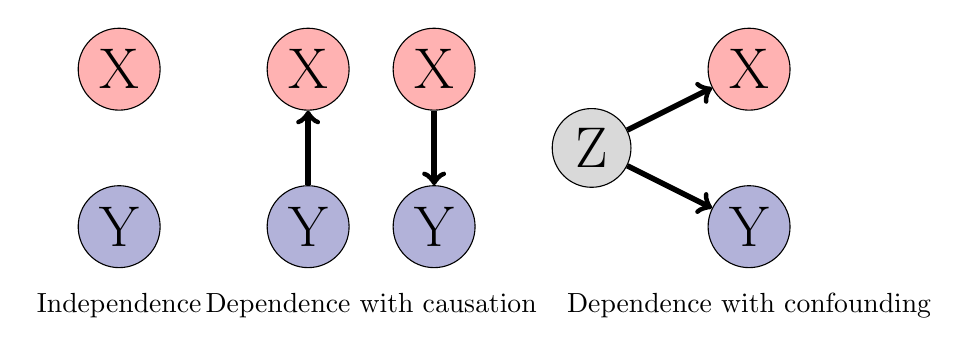
\begin{tikzpicture}[node distance=1.5cm]
% First Diagram: Independence (No Arrows)
\node[draw,circle,fill=red!30,minimum size=1cm,align=center] (A1) at (0,0) {\huge X};
\node[draw,circle,fill=NavyBlue!30,minimum size=1cm,align=center] (B1) at (0,-2) {\huge Y};
\draw[->,opacity=0] (A1) -- (B1);  % No arrow for independence

% Second Diagram: Dependence with Causation (Arrow from B to A)
\node[draw,circle,fill=red!30,minimum size=1cm,align=center] (A2) at (2.4,0) {\huge X};
\node[draw,circle,fill=NavyBlue!30,minimum size=1cm,align=center] (B2) at (2.4,-2) {\huge Y};
\draw[->,line width=2pt] (B2) -- (A2);  % Arrow showing causation from B to A
% Second Diagram: Dependence with Causation (Arrow from B to A)
\node[draw,circle,fill=red!30,minimum size=1cm,align=center] (A2b) at (4,0) {\huge X};
\node[draw,circle,fill=NavyBlue!30,minimum size=1cm,align=center] (B2b) at (4,-2) {\huge Y};
\draw[->,line width=2pt] (A2b) -- (B2b);  % Arrow showing causation from B to A

% Third Diagram: Dependence with Spurious Causation (Arrow from C to A and B)
\node[draw,circle,fill=red!30,minimum size=1cm,align=center] (A3) at (8,0) {\huge X};
\node[draw,circle,fill=NavyBlue!30,minimum size=1cm,align=center] (B3) at (8,-2) {\huge Y};
\node[draw,circle,fill=gray!30,minimum size=1cm,align=center] (C3) at (6,-1) {\huge Z};
\draw[->,line width=2pt] (C3) -- (A3);  % Arrow from C to A
\draw[->,line width=2pt] (C3) -- (B3);  % Arrow from C to B

% Labels for the diagrams
\node[align=center] at (0,-3) {Independence};
\node[align=center] at (3.2,-3) {Dependence with causation};
\node[align=center] at (8,-3) {Dependence with confounding};
\end{tikzpicture}
\end{center}
Consider the following random variables:
    \begin{itemize}
        \item Ice cream sales
        \item Daily high temperature
        \item Daily coast guard emergencies
    \end{itemize}
    They are all correlated - but which relationships are causal?
\end{frame}

\begin{frame}
    \frametitle{Summary}
    So far we have:
    \begin{itemize}
        \item If $Y=X+X'$ then $E[X]=E[X]+E[X']$
        \item If $Y=mX+c$ them $E[Y]=mE[X]+c$
        \item If $Y=X+X'$ then $E[XY]=E[X]E[Y]$ {\bf if $X$ and $X'$ are independent}
        \item If $Y=X+X'$ then $Var(Y)=Var(X)+Var(X)$ {\bf if $X$ and $X'$ are independent}
        \item If $Y=mX+c$ then $Var(X)=m^2Var(X)$
    \end{itemize}
    {\bf\underline{Useful example}} \par 
    Now let $Y=X+X'$, and $Z=2X$ where $X\stackrel{d}{=}X'$ \par
    By the above results, we have: $E[Y]=E[Z]=2E[X]$ \par
    But $Var(Y)=2Var(X)$ and $Var(Z)=4Var(X)$
\end{frame}

\begin{frame}
    \frametitle{Useful examples}
    Let $Y=X+X'$, and $Z=2X$ where $X\stackrel{d}{=}X'$ \par
    By the above results, we have: $E[Y]=E[Z]=2E[X]$ \par
    But $Var(Y)=2Var(X)$ and $Var(Z)=4Var(X)$ \par
    - why are these different? \par
    Now let $W=1-X$. We have $Var(X)=Var(W)$, but what about $Var(X+W)$?
\end{frame}

\begin{frame}
    \frametitle{Useful examples}
    Recall the definitions of equality between random variables:
    \begin{itemize}
        \item $X=X'$ means the outcomes are identical
        \item $X=X'$ means $X$ and $X'$ follow the same distribution
    \end{itemize}
    If $Z=2X$, then $Z=X+X$, where clearly $X=X$ \par
    %$Z=X+X'$ where $X\stackrel{d}{=}X'$
    Let $X$ and $X'$ be the outcomes of rolling $2$ different dice, and $Y=X+X'$. Then we have:
    \begin{eqnarray*}
        p_Y(y) = \left\{\begin{array}{lr}
		\frac 1{36}, & x=2,12\\
            \frac 1{18}, & x=3,11\\
            \frac 1{12}, & x=4,10\\
            \frac 1{9}, & x=5,9\\
            \frac 5{36}, & x=6,8\\
            \frac 1{6}, & x=7\\
			0, & \text{otherwise}
		\end{array}\right.,\qquad
        p_Z(z) = \left\{\begin{array}{lr}
		\frac 1{6}, & x=2,4,6,8,10,12\\
			0, & \text{otherwise}
		\end{array}\right.
    \end{eqnarray*}
    - why does $Z$ have larger variance? \par
    If $W=1-X$ then $Var(X+W)=Var(1)=0$ \par
    - these random variables are not independent!
\end{frame}

\begin{frame}
    \frametitle{Further topics}
    MATH163 will be limited to computations with random variables of the form:
    $$Y=a_1G_1(X_1)+a_2G(X_2)+\dots+a_nG_n(X_n)+c$$
    Or the special case of expectation when:
    $$Y=G_1(X_1)\cdot G_2(X_2)\cdots G_n(X_n)$$
    The more general case $Y=f(X_1,X_2,\dots X_n)$ will be covered in future statistics modules \par
    %We are however touching on some concepts from future statistics modules, namely:
    If interested, feel free to look up the following:
    \begin{itemize}
        \item Joint distributions
        \item Convolutions
        \item Moment generating functions
    \end{itemize}
    - you will NOT be assessed on these ideas this year
    %You are not expected to study these in MATH163, but 
    %- feel free to look them up if you are interested \par
\end{frame}

\begin{frame}
\frametitle{Example}
Let $X$ and $Y$ be two independent uniform random variables on $(0,1)$ and let $Z=(1-X)^2Y$. \par
Find $E[Z]$.
\end{frame}

\begin{frame}
\frametitle{Example}
A factory produces metal rods, and each rod’s diameter and length must meet quality standards. Let $X_1 \sim U(4.8, 5.2)$ be the diameter (in cm) of a randomly selected rod, and $X_2 \sim U(9.8, 10.2)$ be the length (in cm) of a randomly selected rod \par
The Quality Score \( Y \) is defined as:
\[
Y = 50 \left( X_1 - 5 \right)^2 + 30 \left( X_2 - 10 \right)^2
\]
where deviations from the ideal values (5 cm diameter, 10 cm length) lower the score
{\bf\underline{Question}}
\begin{itemize}
    \item[(a)] Compute \( E[Y] \) and \( \text{Var}(Y) \)
    \item[(b)] If the factory improves its cutting precision so that diameter variation is reduced to \( U(4.9, 5.1) \), how does this affect \( E[Y] \)?
    \item[(c)] Interpret why squared deviations are used in quality control and why reducing variability improves quality
\end{itemize}
\end{frame}

\begin{frame}
		\frametitle{Bernoulli distribution}
		%{\bf\underline{Description}} \par
		A single event happens with probability $p$ \par
		
		{\bf\underline{Definition}} \par
		$$
		p_X(k) = \left\{\begin{array}{lr}
			p, & k=1\\
			1-p, & k=0
		\end{array}\right.
		$$
		
		{\bf\underline{Examples}}
		\begin{itemize}
			\item Coin toss ($p=0.5$)
			\item Rolling a double in Monopoly ($p=\frac 16$)
			\item Defective Product Detection
			\item Medical test outcome
			\item Individual customer purchase
			\item Single vote in an election
		\end{itemize}
		%{\small\color{NavyBlue} - these are all single events with binary outcomes}
	Note: we can map any binary outcome space to the set $\{0,1\}$ \par
        A useful application is $\{A,\bar A\}$ for any $A\subseteq\Omega$
	\end{frame}
	
	\begin{frame}
		\frametitle{Bernoulli distribution}
		\begin{columns}
			\column{0.5\textwidth}
			\centering
			\fbox{\includegraphics[width=\textwidth]{bernoulli.png}}
			Bernoulli PMF ($p=0.22$)
			\column{0.5\textwidth}
			\centering
			\fbox{\includegraphics[width=\textwidth]{bernoullicdf.png}}
			Bernoulli distribution CDF ($p=0.22$)
		\end{columns}
		Question: what are the mean, mode, median and variance of a Bernoulli random variable, in terms of $p$?
	\end{frame}
	
	\begin{frame}
		\frametitle{Bernoulli distribution}
		{\bf\underline{Mean}}
		$$E[X]=\sum_ix_iP(X=x_i)=0\times(1-p)+1\times p=\tcboxmath{p}$$
		{\bf\underline{Variance}}
		\begin{eqnarray*}
			Var(X)&=&\sum_i(x_i-\mu)^2P(X=x_i)=(-p)^2(1-p)+(1-p)^2p\\
			&=&p^2(1-p)+(1-p)^2p=p(1-p)(p+1-p)=\tcboxmath{p(1-p)}
		\end{eqnarray*}
		{\bf\underline{Median}}
		$$
		med = \left\{\begin{array}{lr}
			0, & p<\frac 12\\
			\left[0,1\right], & p=\frac 12\\
			1, & p>\frac 12
		\end{array}\right.
		$$
		{\bf\underline{Mode}}
		$$
		mode = \left\{\begin{array}{lr}
			0, & p<\frac 12\\
			\lbrace 0,1\rbrace, & p=\frac 12\\
			1, & p>\frac 12
		\end{array}\right.
		$$
        {\small\color{NavyBlue} - we typically won't discuss the median and mode of a random variable}
	\end{frame}

    
	\begin{frame}
		\frametitle{Binomial distribution}
		There are $n$ things. Choose each of them independently with probability $p$ \par
        - how many do you choose in total? \par
		We count the number of successes in $n$ independent Bernoulli trials \par
		{\bf\underline{Definition}} \par
		\begin{eqnarray*}
			p_X(k)&=&\frac{n!}{k!(n-k)!}p^k(1-p)^{n-k}\\
			&=&{n\choose k}p^k(1-p)^{n-k}
		\end{eqnarray*}
		%$^*$We will discuss this in week 4, alongside mean and variance \par
		The binomial distribution requires:
		\begin{itemize}
			\item A fixed number of trials
			\item Two possible outcomes per trial
			\item Constant probability of success across trials
			\item Independence of trials
		\end{itemize}
	\end{frame}
	
	\begin{frame}
		\frametitle{Binomial distribution}
		{\bf\underline{Examples}} \par
		\begin{itemize}
			\item The number of defective products in a sample of 20 items randomly selected from a production line
			\item The number of patients who test positive for a disease out of 50 tested patients, assuming a known probability of a positive result
			\item The number of customers out of 100 who purchase a product after a sales pitch
			\item The number of voters who vote for Candidate A in a sample of 500 voters
		\end{itemize}
		{\small\color{NavyBlue} - a good way to identify candidates for a binomial distribution is the ``out of $n$" property} \par
		{\bf\underline{Discussion}} \par
		When would you need to be careful using a binomial distribution to model these phenomena?
	\end{frame}
	
	\begin{frame}
		\frametitle{Binomial distribution}
		\begin{columns}
			\column{0.5\textwidth}
			\centering
			\fbox{\includegraphics[width=\textwidth]{binomial.png}}
			Binomial distribution PMF ($n=20$)
			\column{0.5\textwidth}
			\centering
			\fbox{\includegraphics[width=\textwidth]{binomialcdf.png}}
			Binomial distribution CDF ($n=20$)
		\end{columns}
		{\small\color{NavyBlue} - this is a discrete random variable. Values of the PMF are dots, and the dots are connected for ease of visualisation} \par
        Dashed lines show the the PDF for $1-p$ \par
		Note: the PMF is symmetric under the transformation $x\mapsto n-x,\ p\mapsto 1-p$ \par %(dashed lines) 
        - why?
	\end{frame}
	
	\begin{frame}
		\frametitle{Binomial distribution: mean and variance}
		{\bf\underline{Mean}}
		$$E[X]=\sum_ix_iP(X=x_i)=\sum_{k=1}^nk\times\frac{n!}{k!(n-k)!}p^k(1-p)^{n-k}=\dots$$
		{\bf\underline{Variance}}
		$$Var(X)=\sum_i(x_i-\mu)^2P(X=x_i)=\dots$$
		{\bf There is a quick way!} \par
		Observe: a binomial random variable is a sum of $n$ {\bf independent and identically distributed (i.i.d.)} $n$ Bernoulli random variables \par %with parameter $p$ \par 
        {\small\color{NavyBlue} - ``identical" here means they have the same parameter $p$} \par
		%{\small\color{NavyBlue} - we will cover this in the section ``computations with random variables"} \par 
		{\bf\underline{Mean}}
		$$\tcboxmath{E[X]=np}$$
		{\bf\underline{Variance}}
		$$\tcboxmath{Var(X)=np(1-p)}$$
	\end{frame}

    \begin{frame}
		\frametitle{Example}
		In a committee, two independent groups of voters make decisions on a proposal. Each voter independently votes \textbf{``yes''} with a certain probability. The total number of ``yes" votes from both groups determines whether the proposal passes. Let:
    \begin{itemize}
        \item $X$ be the number of ``yes" votes from \textbf{Group A}, where $4$ voters each vote independently with probability $0.5$ of voting ``yes"
        \item $Y$ be the number of ``yes" votes from \textbf{Group B}, where $3$ voters each vote independently with probability $0.6$ of voting ``yes"
    \end{itemize}
\textbf{Questions:}
\begin{enumerate}[(a)]
    \item Compute the probability that the total number of yes votes $Z$ is $3$
    \item Compute $E[Z]$ and $\text{Var}(Z)$
    \item If the proposal is approved when at least $4$ votes are ``yes", determine the probability that the proposal is approved
    \item Discuss the assumptions behind modeling voting behavior as independent Bernoulli trials and potential limitations of this assumption in real-world scenarios
\end{enumerate}
\end{frame}

%%%%%%%%%%%%%%%%%%%%%%%%%%%%%%%%%%%%%%%%%%%%%%%%%%%%%%%%%%%%%%%%
%%%%%%%%%%%%%%%%%%%%%%%%%%%%%%%%%%%%%%%%%%%%%%%%%%%%%%%%%%%%%%%%

\section{Week 5: random variable models I}
	
	\begin{frame}
		\frametitle{Common distributions}
		\begin{itemize}
            \item {\bf Uniform:} everything equally likely $\checkmark$
			\item {\bf Bernoulli:} success or failure $\checkmark$
			\item {\bf Binomial:} number of successes in $n$ independent trials $\checkmark$
			\item {\bf Geometric:} failures before first success
			\item {\bf Negative binomial:} failures before first $r$ successes
            \item {\bf Hypergeometric:} number of successes in $n$ independent trials without replacement
			\item {\bf Poisson:} constant rates
			\item {\bf Exponential:} ``memoryless"
			\item {\bf Power laws:} growth property
			\item {\bf Normal:} strangely appears everywhere
			\item {\bf $\chi^2$ distribution:} sums of squares of normals
			\item {\bf t-distribution:} extension of normal (c.f. sampling)
		\end{itemize}
	\end{frame}

    \begin{frame}
		\frametitle{Notation}
        The symbol ``$\sim$" means ``is distributed". Standard notations include:
		\begin{itemize}
            \item {\bf Uniform:} $X\sim U(a,b)$ or $X\sim Unif(a,b)$
			\item {\bf Bernoulli:} $X\sim Bern(p)$
			\item {\bf Binomial:} $X\sim B(n,p),\ X\sim Bin(n,p)$
			\item {\bf Geometric:} $X\sim G(p)$
			\item {\bf Negative binomial:} $X\sim NB(r,p)$
            \item {\bf Hypergeometric:} $X\sim H(K,N-K,n)$
			\item {\bf Poisson:} $X\sim P(\lambda),\ X\sim Po(\lambda),\ X\sim Pois(\lambda)$
			\item {\bf Exponential:} $X\sim Exp(\lambda)$
			\item {\bf Power laws:} ($p_X(k)\propto k^{-\lambda},\ f_Y(y)\propto y^{-\lambda}$)
			\item {\bf Normal:} $X\sim N(\mu,\sigma^2)$
			\item {\bf $\chi^2$ distribution:} sums of squares of normals $X\sim\chi^2(\nu)$
			\item {\bf t-distribution:} $X\sim t_{\nu}$ - ``$\nu$" is a parameter
		\end{itemize}
	\end{frame}

\begin{frame}
\frametitle{Fun example}
The St. Petersburg lottery is played as follows:
\begin{itemize}
    \item A player pays an ante of $\$A$ to enter
    \item Round $1$: $\$2$ prize is placed down and a coin is tossed \par
    HEADS you take the prize money, TAILS you continue to round $2$
    \item Round $2$: the prize money is doubled and a coin is tossed \par
    HEADS you take the prize money, TAILS you continue to round $3$ 
    \item Round $i$: the prize money is doubled and a coin is tossed \par
    HEADS you take the prize money, TAILS you continue to round $i+1$
\end{itemize}
{\bf\underline{Questions}}
\begin{enumerate}
    \item What is the expected amount of money won?
    %\item What is the expected number of rounds before the game ends?
    \item If you ran the casino, what would you charge as the ante?
\end{enumerate}
\end{frame}

\begin{frame}
\frametitle{Fun example}
{\bf\underline{Answers}} \par
The key is to define random variables: \par
Let $X$ be the number of rounds played and $Y$ be the total won - then $Y=2^X$ \par
The game stops at round $k$ if $k-1$ tails are tossed in a row, followed by $1$ head \par
There is only one way for this to happen, and each toss happens independently, so: 
$$P(X=k)=\left(\frac 12\right)^k$$
%$i\mapsto 2^i$ is $1-1$ and so we have:
%$$P(Y=2^i)=\left(\frac 12\right)^2$$
Crucially, we can calculate:
$$E[Y]=\sum_{k=1}^{\infty}2^k\frac 1{2^k}$$
...which diverges!
Note, however, the expected number of rounds is:
$$E[X]=\sum_{k=1}^{\infty}k\frac 1{2^k}$$
And this sum converges to $2$ (proof omitted) \par
- are these sums familiar from calculus?
%{\bf We will revisit this example when studying the geometric distribution} \par
%- homework: revise the geometric series
%Here, we have $X=Y$ - the strongest equality between random variables! \par
%{\bf This answer is beyond the scope of assessment in MATH163 as it includes some theory from other courses}
\end{frame}

\begin{frame}
		\frametitle{Geometric distribution $G(p)$}
		Consider repeated Bernoulli trials (e.g. roll a dice, success$=6$) \par 
		The binomial measures number of successes in $n$ trials \par 
		Geometric distribution measures:
		\begin{itemize}
			\item Number of trials to to the first success
			\item OR number of failures before the first successes\qquad$\leftarrow$ we will use this one
		\end{itemize}
		{\small\color{NavyBlue} - these $2$ definitions are ``$1$ out" from each other \par
			- the geometric distribution only has $1$ parameter, $p$} \par
		{\bf\underline{Exercise}} \par
		Write down an expression for $p_X(k)$
		\begin{center}
			\fbox{\includegraphics[width=.2\textwidth]{countdown.jpg}}
		\end{center}
	\end{frame}
	
	\begin{frame}
		\frametitle{Geometric distribution $G(p)$}
		PMF:
		$$p_X(k)=p(1-p)^k$$
		CDF:
		\begin{eqnarray*}
			P(X\leq k)&=&\sum_{i=0}^kp(1-p)^i\\
			&=&\dots=1-(1-p)^{k+1}\\
			\Rightarrow P(X\leq x)&=&1-(1-p)^{\lfloor x\rfloor+1}\quad (x\geq0)
		\end{eqnarray*}
		{\small\color{NavyBlue} - this should be familiar as the ``geometric series" \par
			- the geometric distribution only has $1$ parameter, $p$ \par
			- technically we should write all CDFs in terms of a continuous variable $x$ \par
			- there are no binomial coefficients in these expressions, precisely because order matters} \par
            Recall the {\it geometric series} from calculus:
            $$\sum_{i=0}^kar^i\xrightarrow{k\rightarrow\infty}\frac a{1-r}\quad\text{if}\ |r|<1$$
	\end{frame}
	
	\begin{frame}
		\frametitle{Geometric distribution $G(p)$}
		{\bf\underline{Mean}} \par
		We can calculate the mean of a geometric random variable from first principles. \par
		%Recall the geometric series: $\sum_{i=0}^{\infty}ar^i=\frac a{1-r}\quad (|r|<1)$ \par 
		We have:
		\begin{eqnarray*}
			E[X]:&=&\sum_{k=0}^{\infty}kp(1-p)^k\\
			&=&p(1-p)\sum_kk(1-p)^{k-1}\\
			&=&-p(1-p)\frac d{dp}\sum_k(1-p)^k\\
			&=&p(1-p)\frac d{dp}\frac 1p\quad (a=1,\ r=1-p)\\
			&=&p(1-p)p^{-2}=\tcboxmath{\frac{1-p}p}
		\end{eqnarray*}
		Careful: the other definition (trials to first success) has mean $E[X]=\frac 1p$
	\end{frame}
	
	\begin{frame}
		\frametitle{Geometric distribution $G(p)$}
		{\bf\underline{Variance}} \par
		The working is similar to the case for the mean:
		\begin{eqnarray*}
			\text{Note}\quad \frac{d^2}{dp^2}(1-p)^k&=&(k^2-k)(1-p)^{k-2}\\
			Var(X):&=&\sum_{k=0}^{\infty}k^2p(1-p)^k-E[X]^2\\
			&=&p(1-p)^2\frac{d^2}{dp^2}\sum_k(1-p)^k+p(1-p)\sum_kk(1-p)^{k-1}-E[X]^2\\
			&=&p(1-p)^2\frac{d^2}{dp^2}\frac 1p+E[X]-E[X]^2\\
			&=&2p(1-p)^2p^{-3}+\frac{1-p}p-\left(\frac{1-p}p\right)^2\\
			&=&\left(\frac{1-p}p\right)^2+\frac{1-p}p=\tcboxmath{\frac{1-p}{p^2}}
		\end{eqnarray*}
	\end{frame}
	
	\begin{frame}
		\frametitle{Geometric distribution $G(p)$}
		\begin{columns}
			\column{0.5\textwidth}
			\centering
			\fbox{\includegraphics[width=\textwidth]{geometric.png}}
			Geometric distribution PMF
			\column{0.5\textwidth}
			\centering
			\fbox{\includegraphics[width=\textwidth]{geometriccdf.png}}
			Geometric distribution CDF
		\end{columns}
		\vspace{5pt}
		Note: the geometric PMF is always monotone decreasing in $x$ - why?
	\end{frame}
	
	\begin{frame}
		\frametitle{Geometric distribution $G(p)$}
		The Geometric distribution describes ``time to the first something" in independent Bernoulli trials, e.g. time to first head in repeated coin tosses \par
		Note: if we have tossed $n$ tails in a row, the distribution of tosses required before the next head is unchanged: this is due to {\it independence} \par
		This property is known as {\it memorylessness} - formally we say:
		$$P(X\geq n+m\vert X\geq n)=P(X\geq m)$$
		%{\bf\underline{Exercise}} \par
		%Show that the geometric distribution is memoryless \par
		{\bf\underline{Theorem}} \par
		The geometric distribution is memoryless, and is the only such discrete random variable
	\end{frame}

	\begin{frame}
		\frametitle{Geometric distribution $G(p)$}
		{\bf\underline{Theorem}} \par
		The geometric distribution is memoryless, and is the only such discrete random variable
        {\bf\underline{Proof}} \par
        We want to prove that:
        $$P(X\geq n+m\vert X\geq n)=P(X\geq m)\Leftrightarrow p_X(k)=p(1-p)^k\ \forall k\in\{0,1,2,\dots\},\ p\in(0,1)$$
		Part 1: geometric $\Rightarrow$ memoryless
        \begin{eqnarray*}
            P(X\geq n+m\vert X\geq n)&=&\frac{P(X\geq n+m\cap X\geq n)}{P(X\geq n)}\\
            &=&\frac{P(X\geq n+m)}{P(X\geq n)}\quad\bigstar\\
            &=&\frac{(1-p)^{m+n}}{(1-p)^m}\\
            &=&(1-p)^n\\
            &=&P(X\geq n)
        \end{eqnarray*}
	\end{frame}

	\begin{frame}
		\frametitle{Geometric distribution $G(p)$}
		{\bf\underline{Proof}} \par
		Part 2: memoryless $\Rightarrow$ geometric
        \begin{eqnarray*}
            \bigstar\Rightarrow \frac{P(X\geq n+m)}{P(X\geq n)}&=&P(X\geq m)\quad\text{(memoryless property)}\\
            \Rightarrow P(X\geq m+n)&=&P(X\geq m)P(X\geq n)
        \end{eqnarray*}
        We use the exponential functional equation: $g(m+n)=g(m)g(n)\Rightarrow g(k)=c^k,\ c>0$ \par
        This gives:
        \begin{eqnarray*}
            p_X(k)&=&P(X\geq k)-P(X\geq k+1)\quad\text{(discrete property)}\\
            &=&c^{k}-c^{k+1}\\
            &=&c^{k}(1-c)
        \end{eqnarray*}
        Setting $c=1-p\in(0,1)$ gives:
        $$p_X(k)=p(1-p)^{k}\quad\blacksquare$$
	\end{frame}

\begin{frame}
\frametitle{Fun example (continued)}
We generalize the St Petersburg Lottery as follows: \par
Each round the prize money increases by a factor $\alpha>1$ (previously $\alpha=2$) \par
We replace the coin toss with a different Bernoulli random variable with probability of success $p$ \par
{\small\color{NavyBlue} - ``success" means the game {\it stops} \par
- we can think of this as tossing a biased coin}

\begin{itemize}
    \item A player pays an ante of $\$A$ to enter
    \item Round $1$: $\$\alpha$ prize is placed down and a {\it biased} coin is tossed \par
    HEADS you take the prize money, TAILS you continue to round $2$
    \item Round $i$: the prize money is doubled and a coin is tossed \par
    HEADS you take the prize money, TAILS you continue to round $i+1$
\end{itemize}
{\bf\underline{Questions}}
\begin{enumerate}
    \item What is the expected amount of money won?
    \item If you ran the casino, what would you charge as the ante?
\end{enumerate}
\end{frame}

\begin{frame}
\frametitle{Fun example (continued)}
{\bf\underline{Answers}} \par
Let $X$ be the number of rounds played and $Y$ be the total won - then $Y=\alpha^X$ \par
The game stops at round $k$ if $k-1$ failures occur in a row, followed by $1$ success \par
If $X$ is the number of rounds played then:
$$P(X=k)=\dots$$
%$i\mapsto 2^i$ is $1-1$ and so we have:
%$$P(Y=2^i)=\left(\frac 12\right)^2$$
Recall if $Y=G(X)$ then $E[Y]=\sum_xG(X)p_X(x)$ \par
The expected payback is:
\begin{eqnarray*}
    E[Y]&=&\sum_{k=1}^{\infty}\dots\\
    &=&\sum_{k=1}^{\infty}ar^{k-1}\quad\text{(find $a$ and $r$)}\\
    &=&\sum_{k=0}^{\infty}ar^k\\
    &=&\frac a{1-r}
\end{eqnarray*}


\end{frame}
	
	\begin{frame}
		\frametitle{Negative binomial distribution $NB(r,p)$}
		Generalise the geometric distribution:
		\begin{itemize}
			\item Number of trials to $r$ successes
			\item Number of failures before $r$ successes\qquad$\leftarrow$ we will use this one
		\end{itemize}
		Note: this is just $r$ consecutive, independent geometric random variables! \par
        PMF:
        $$p_X(k)={k+r-1 \choose k}(1-p)^kp^r$$
        {\bf\underline{Mean}} \par
        $$E[X]=\frac{r(1-p)}{p}$$
        {\bf\underline{Variance}} \par
        $$Var(X)=\frac{r(1-p)}{p^2}$$
	\end{frame}
	
	\begin{frame}
		\frametitle{Negative binomial distribution $NB(r,p)$}
		\begin{columns}
			\column{0.5\textwidth}
			\centering
			\fbox{\includegraphics[width=\textwidth]{negbinom.png}}
			Negative binomial distribution PMF ($r=5$)
			\column{0.5\textwidth}
			\centering
			\fbox{\includegraphics[width=\textwidth]{negbinomcdf.png}}
			Negative binomial distribution CDF ($r=5$)
		\end{columns}
	\end{frame}

    \begin{frame}
		\frametitle{Negative binomial distribution $NB(r,p)$}
		{\bf\underline{Example}} \par
        A sales employee must meet a quota of 3 successful sales before the end of the day. Each time they call a customer, the probability of making a successful sale is 0.2 \par
        Let \( X \) be the number of failed calls before reaching the 3rd successful sale
        To analyze the time spent on unsuccessful calls, suppose each failed call takes 5 minutes, and each successful sale takes 10 minutes and let $Y$ be the total time (in minutes) until the employee meets their quota.
\begin{enumerate}
    \item[(a)] Write down the probability mass function (PMF) of \( X \)
    \item[(b)] What is the probability that the employee makes at least one unsuccessful call?
    \item[(c)] Find the expectation and variance of \( X \)
    \item[(d)] Write down the expectation and variance of \( Y \)
    \item[(e)] Explain why \( Y \) does not follow a Negative Binomial distribution and interpret the variance of $Y$
    \item[(f)] Suggest a way of improving this model
\end{enumerate}
	\end{frame}

    \begin{frame}
	\frametitle{Hypergeometric distribution $H(K,N-K,n)$}
    %\vspace{5pt}
        %\begin{columns}[b]
	%\column{0.7\textwidth}
        A bag of snooker balls contains $15$ red balls and $6$ other colours. You select $5$ balls at random. What is the probability that exactly $3$ of them are red? \\~\\
	Binomial: probability of $k$ successes in $n$ {\it independent} trials \par
        - this only applies if we select {\it with replacement} \\~\\
        When sampling without replacement, we get the {\bf hypergeometric distribution} \\~\\
        %\column{0.3\textwidth}
        \begin{center}
        \fbox{\includegraphics[width=.3\textwidth]{snooker.jpg}} \par
        The white ball doesn't count!
        \end{center}
        %\end{columns}
    \end{frame}
    \begin{frame}
    
	\frametitle{Hypergeometric distribution $H(K,N-K,n)$}
    %\vspace{5pt}
        %\begin{columns}[b]
	%\column{0.7\textwidth}
        {\color{gray}
        A bag of snooker balls contains $15$ red balls and $6$ other colours. You select $5$ balls at random. What is the probability that exactly $3$ of them are red? \\~\\
        }
        \begin{itemize}
            \item $N$ is the population size ($16$ balls)
            \item $n$ is the sample size ($5$ balls)
            \item $K$ is the number of ``success states" ($15$ red balls)
            \item $k$ is the number of observed successes ($3$ red balls)
        \end{itemize}
        PMF:
        $$p_X(k)=\frac{{K\choose k}{N-K\choose n-k}}{{N\choose n}}$$
        We have:
        \begin{itemize}
            \item ${K\choose k}$ ways of choosing $3$ red balls from $15$
            \item ${N-K\choose n-k}$ ways of choosing $2$ non-red balls from $6$
            \item ${N\choose n}$ ways of choosing $5$ balls from $21$
        \end{itemize}
        Notation: $X\sim H(K,N-K,n)$
        %\column{0.3\textwidth}
        %\fbox{\includegraphics[width=\textwidth]{snooker.jpg}}
        %${K\choose k}$ ways of choosing $3$ red balls from $15$ \par\vspace{5pt}
        %${N-K\choose n-k}$ ways of choosing $2$ non-red balls from $6$\par\vspace{5pt}
        %${N\choose n}$ ways of choosing $5$ balls from $21$ \par\vspace{5pt}
        %The white ball doesn't count!
        %\end{columns}
    \end{frame}

    \begin{frame}
	\frametitle{Hypergeometric distribution $H(K,N-K,n)$}
        {\bf\underline{Mean}} \par
        $$E[X]=n\frac KN$$
        {\bf\underline{Variance}} \par
        $$Var(X)=n\frac KN\frac{N-K}N\frac{N-n}{N-1}$$
        (proofs omitted) \par 
        {\bf\underline{Question}} \par
        How many fish are there in a lake? \par
        - can you count them without draining the lake and counting dead fish? \par 
        - which distribution describes uncertainty in this measurement?
    \end{frame}

    \begin{frame}
	\frametitle{Hypergeometric distribution $H(K,N-K,n)$}
        {\bf\underline{Answer}} \par
        YES - capture, mark, recapture (CMR) \par
        \begin{itemize}
            \item There are $N$ fish in the lake
            \item We sample $K$ of them and mark them
            \item Release those $K$ fish - now $K/N$ of the fish are marked
            \item Capture another sample of size $n$ and let $k$ be the number that are marked
            \item If $X$ is a random variable denoting number of marked fish recaptured, then $X$ is hypergeometric distributed (with $,n,K,k$ as on the previous slide)
            \item We can now estimate $N$: $\frac KN\approx \frac kn\Rightarrow N\approx \frac{Kn}k$
            %\item We have $E[K]=\frac nN$ so our estimate $\hat N=\frac{E[K]}n=\frac{Mn}{k}$
        \end{itemize}
    \end{frame}

        \begin{frame}
	\frametitle{Hypergeometric distribution $H(K,N-K,n)$}
        {\bf\underline{Answer}} \par
        Formally, $\hat N:=\frac{Kn}k$ is an {\it estimator} of $N$ \par
        Note: $k$ follows a hypergeometric distribution with mean $n\frac KN$ \par
        %The accuracy of the estimator $\hat N$ is dependent on the variance of $X$ \par
        - we will revisit this example later in the course! \par
        Assumptions:
        \begin{itemize}
            \item No marked fish are lost between samples
            \item All fish have an equal chance of being captured (homogeneous mixing)
            \item The population is closed (no immigration, emigration, births, or deaths)
        \end{itemize}
    \end{frame}

\begin{comment}
    \begin{frame}
		\frametitle{Poisson distribution}
		Independent events happen at a fixed rate $\lambda$ (per unit time) \par
		{\small\color{NavyBlue} - for example, ambulances arriving at a hospital. Can we assume there are independent?} \par
		More generally, points are placed independently in space with mean density $\lambda$ \par
		PMF: $p_X(k)$ denotes the probability that exactly $k$ events occur within a time interval \par
		{\small\color{NavyBlue} - use a fixed time interval of one hour in out ambulance example} \par
		We can derive a formula for $p_X(k)$ by using the binomial distribution
	\end{frame}
    \end{comment}
	
	\begin{frame}
		\frametitle{Poisson distribution $Pois(\lambda)$}
		Poisson {\it process:} independent events happen at a fixed rate $\lambda$ (per unit time) \par
		{\small\color{NavyBlue} - for example, ambulances arriving at a hospital. Can we assume they are independent?} \par
		More generally, points are placed independently in space with mean density $\lambda$ \par
		Poisson {\it distribution:} number of events occuring in a given interval \par
		PMF: $p_X(k)$ denotes the probability that exactly $k$ events occur within a time interval \par
		{\small\color{NavyBlue} - use a fixed time interval of one hour in our ambulance example} \par
		We can derive a formula for $p_X(k)$ by using the binomial distribution
	\end{frame}
	
	\begin{frame}
		\frametitle{Poisson distribution $Pois(\lambda)$}
		Deriving Poisson from binomial:
		\begin{itemize}
			\item Divide the hour into $n$ intervals, assuming at most $1$ ambulance can arrive per interval
			\item Each interval is one Bernoulli trial - yes or no
			\item We need $n\geq\lambda$ - why?
			\item This approximates $Pois(\lambda)$ with $Bin(n,\frac{\lambda}n)$
			\item Take the limit $n\rightarrow\infty$ keeping $\lambda=np$ constant
		\end{itemize}
	\end{frame}
	
	\begin{frame}
		\frametitle{Poisson distribution $Pois(\lambda)$}
		\begin{eqnarray*}
			p_X(k)%&=&\lim_{n\rightarrow\infty}{n\choose k}\left(\frac{\lambda}n\right)^k\left(1-\frac{\lambda}n\right)^{n-k}\\
			&=&\lim_{n\rightarrow\infty}\frac{n!}{k!(n-k)!}\left(\frac{\lambda}n\right)^k\left(1-\frac{\lambda}n\right)^{n-k}\\
			&=&\frac{\lambda^k}{k!}\lim_{n\rightarrow\infty}\underbrace{\frac{n!}{(n-k)!}\left(\frac 1{n^k}\right)}_A\underbrace{\left(1-\frac{\lambda}n\right)^n}_B\underbrace{\left(1-\frac{\lambda}n\right)^{-k}}_C
		\end{eqnarray*}
	\end{frame}
	
	\begin{frame}
		\frametitle{Poisson distribution $Pois(\lambda)$}
		\begin{eqnarray*}
			A:\ \lim_{n\rightarrow\infty}\frac{n!}{(n-k)!}\left(\frac 1{n^k}\right)&=&\lim_{n\rightarrow\infty}\frac{n(n-1)(n-2)\dots(n-k+1)}{n^k}\\
			&=&\lim_{n\rightarrow\infty}\frac{n}{n}\frac{(n-1)}{n}\frac{(n-2)}{n}\dots\frac{(n-k+1)}{n}\\
			&=&1\\
			\\
			C:\ \lim_{n\rightarrow\infty}\left(1-\frac{\lambda}n\right)^{-k}&=&1
		\end{eqnarray*}
	\end{frame}
	
	\begin{frame}
		\frametitle{Poisson distribution $Pois(\lambda)$}
		\begin{eqnarray*}
			\text{We now have:}\quad p_X(k)&=&\frac{\lambda^k}{k!}\lim_{n\rightarrow\infty}\left(1-\frac{\lambda}n\right)^n\\
			\text{Recall:}\quad e:&=&\lim_{m\rightarrow\infty}\left(1+\frac 1m\right)^m\\
			\text{Let}\ m=-\frac n{\lambda},\ \text{then}\ \lim_{n\rightarrow\infty}\left(1-\frac{\lambda}n\right)^n&=&\lim_{m\rightarrow\infty}\left(1+\frac 1m\right)^{m(-\lambda)}\\
			&=&e^{-\lambda}
			%\text{So}\quad P(X=k)&=&\frac{\lambda^k}{k!}e^{-\lambda}
		\end{eqnarray*}
		So
		$$
		\tcboxmath{
			p_X(k)=\frac{\lambda^k}{k!}e^{-\lambda}
		}$$%\boxed
		{\small\color{NavyBlue} - this formula should be familiar!}%: the Poisson distribution is the limiting case of the binomial distribution as $n\rightarrow\infty$ keeping $np$ constant}
\end{frame}

\begin{frame}
	\frametitle{Poisson distribution $Pois(\lambda)$}
	\begin{columns}
		\column{0.5\textwidth}
		\centering
		\fbox{\includegraphics[width=\textwidth]{poisson.png}}
		Poisson distribution PMF
		\column{0.5\textwidth}
		\centering
		\fbox{\includegraphics[width=\textwidth]{poissoncdf.png}}
		Poisson distribution CDF
	\end{columns}
\end{frame}

\begin{frame}
	\frametitle{Poisson distribution $Pois(\lambda)$}
    {\bf\underline{Mean}} \par
    In taking the limit $n\rightarrow\infty$ keeping $np=\lambda$ constant, we have:
    $$E[X]=\lambda$$
    {\bf\underline{Variance}} \par
    As $n\rightarrow\infty$, we have $p=\frac{\lambda}n\rightarrow 0$ and so $1-p\rightarrow 1$ \par
    $Var(X)=np(1-p)\rightarrow\lambda\times 1=\lambda$, i.e.:
    $$Var(X)=\lambda$$
    Observe:
    \begin{itemize}
        \item {\bf In the Poisson distribution, $E[X]=Var(X)=\lambda$ \par
    - the Poisson distribution only has one parameter!}
    \item Note that in the binomial distribution, $E[X]=np>np(1-p)=Var(X)$
    \item {\bf $Pois(np)$ approximates $Bin(n,p)$ for large $n$ and small $p$}
    \end{itemize}
\end{frame}





    %%%%%%%%%%%%%%%%%%%%%%%%%%%%%%%%%%%%%%%%%%%%%%%%%%%%%%%%%%%%%%%%
    %%%%%%%%%%%%%%%%%%%%%%%%%%%%%%%%%%%%%%%%%%%%%%%%%%%%%%%%%%%%%%%%
\section{Week 6: random variable models II}
\begin{frame}
	\frametitle{Exponential distribution}
	What is the distribution of time between events in a Poisson process \par
	{\small\color{NavyBlue} - in our example, if I record the times between ambulances arriving, how are they distributed?\par
		- we can talk about ``time between events" or ``time until next event" interchangeably - why?}\par
	Let $T$ be a random variable denoting time to next event \par%, then the CDF of $T$ is P(T\leq T)\par 
	$P(T>t)=P(Y=0)$, where $Y\sim Pois(\lambda t)$\par
	$P(Y=0)=\frac{(\lambda t)^0}{0!}e^{-\lambda t}=e^{-\lambda t}$\par
	{\small\color{NavyBlue} - $\lambda$ is a mean per hour, and $t$ denotes a specified number of hours, so we are effectively converting to a new time period specified by $t$, with mean occurances $\lambda t$}\par
	This gives $P(T\leq t)=1-e^{-\lambda t}$\par
	- but this is the CDF of the distribution we are looking for
\end{frame}

\begin{frame}
	\frametitle{Exponential distribution $Exp(\lambda)$}
	{\bf\underline{Definition}} \par
	$$f_T(t)=\lambda e^{-\lambda t},\ \lambda>0$$ \par%\boxed
    {\bf\underline{Mean}} \par
    $$E[X]=\frac 1{\lambda}$$
    {\bf\underline{Variance}}
    $$Var(X)=\frac 1{\lambda^2}$$
    Exercise: derive these expressions \par
    Hint: use integration by parts
\end{frame}

\begin{frame}
	\frametitle{Exponential distribution $Exp(\lambda)$}
        Note: since events in a Poisson process are independent, the time to next event does not depend on past events \par
        Is this property familiar?
        $$P(T>t+a\vert T>a)=P(T>t)\ \forall a,t\geq 0$$
        {\bf\underline{Theorem}} \par
        The exponential distribution is memoryless and is the only such continuous distribution \par
\end{frame}

\begin{frame}
	\frametitle{Exponential distribution $Exp(\lambda)$}
        {\bf\underline{Theorem}} \par
        The exponential distribution is memoryless and is the only such continuous distribution \par
        {\bf\underline{Proof}} \par
        We want to prove that:
        $$P(T>t+a\vert T>a)=P(T>t)\Leftrightarrow f_T(t)=\lambda e^{-\lambda t}$$
        Part 1: exponential $\Rightarrow$ memoryless \par
        Exercise
        \begin{center}
		\fbox{\includegraphics[width=.2\textwidth]{countdown.jpg}}
	\end{center}
\end{frame}

\begin{frame}
	\frametitle{Exponential distribution $Exp(\lambda)$}
        {\bf\underline{Proof}} \par
        Part 2: memoryless $\Rightarrow$ exponential
        \begin{eqnarray*}
            P(T>t+a\vert T>a)&=&P(T>t)\quad\text{memoryless property}\\
            \Rightarrow \frac{P(T>t+a\cap T>a)}{P(T>a)}&=&P(T>t)\quad\text{(Bayes' rule)}\\
            \Rightarrow P(T>t+a\cap T>a)=P(T>t+a)&=&P(T>t)P(T>a)\\
            %\Rightarrow P(T>t)&=&e^{-\lambda t}\quad\text{(exponential functional equation)}
            \end{eqnarray*}
        \color{NavyBlue}
        Observe: $g(t+a)=g(t)g(a)\Rightarrow g(2t)=g(t)^2,\ g(bt)=g(t)^b,\ g(t)=g(1)^t$, so:
        \color{black}
        $$P(T>t)=P(T>1)^{t}$$
        And we can write $P(T>1)=e^{-\lambda}$ for some $\lambda>0$. This gives: \par
        $$f_T(t):=\frac d{dt}\left(1-P(T>t)\right)=\lambda e^{-\lambda}\quad\blacksquare$$
\end{frame}

\begin{frame}
	\frametitle{Exponential distribution $Exp(\lambda)$}
	\begin{columns}
		\column{0.5\textwidth}
		\centering
		\fbox{\includegraphics[width=\textwidth]{exponential.png}}
		Exponential distribution PMF
		\column{0.5\textwidth}
		\centering
		\fbox{\includegraphics[width=\textwidth]{exponentialcdf.png}}
		Exponential distribution CDF
	\end{columns}
\end{frame}

\begin{frame}
	\frametitle{Exponential distribution $Exp(\lambda)$}
        Note the similarity between the exponential distribution and the geometric distribution \par
        They are the continuous/discrete versions of the same process:
        \begin{itemize}
            \item ``Steps to fist success", ``time to next event"
            \item Successes are independent
            \item Add one to $x$, multiple $p_X(x)$ or $f_X(x)$ by a constant \par
                  - that constant is $(1-p)$ or $e^{-\lambda}$ respectively
        \end{itemize}
\end{frame}

\begin{frame}
	\frametitle{Uniform distribution $U(a,b)$}
        Recall the continuous uniform distribution: \par
        {\bf\underline{Definition}} \par
        \begin{eqnarray*}
            f_X(x):&=&\left\{\begin{array}{lr}
			\frac{1}{b-a}, & x\in (a,b)\\
			0, & \text{otherwise}
		\end{array}\right.\\
            F_X(x):&=&\left\{\begin{array}{lr}
            0, & x\leq a\\
			\frac{x-a}{b-a}, & x\in (a,b)\\
			1, & x\geq a
		\end{array}\right.
        \end{eqnarray*}
        {\bf\underline{Mean}}
        $$E[X]=\frac 12(a+b)$$
        {\bf\underline{Variance}}
        $$Var(X)=\frac 1{12}(b-a)^2$$
\end{frame}

\begin{frame}
	\frametitle{Uniform distribution $U(a,b)$}
	\begin{columns}
		\column{0.5\textwidth}
		\centering
		\fbox{\includegraphics[width=\textwidth]{uniform.png}}
		Uniform distribution PDF
		\column{0.5\textwidth}
		\centering
		\fbox{\includegraphics[width=\textwidth]{uniformcdf.png}}
		Uniform distribution CDF
	\end{columns}
\end{frame}

\begin{frame}
	\frametitle{Change of variables formula}
    Let $X$ be a continuous random variable and $Y=G(X)$ for some strictly monotone function $G$ \par
	Given the PDF $F_X(x)$, recall the $5$-step process for deriving $f_Y(y)$ \par
    The general approach is as follows:
        $$f_X(x)dx\approx P(y\leq Y\leq y+dy)=P(y\leq G(X)\leq y+dy)=P(x\leq X\leq x+dx)\approx f_Y(y)dy$$
    {\small\color{NavyBlue} - note thet $dy$ is the change in $y$ when $x$ changes by $dx$} \par
    We have:
    $$\frac{dy}{dx}=G'(x)\Rightarrow dy=G'(x)dx\Rightarrow dx=\frac{dy}{G'(x)}$$
    This gives:
    $$f_Y(y)dy=f_X(x)dx=f_X(x)\frac{dy}{|G'(x)|}$$
    {\small\color{NavyBlue} - we need to use the absolute value of $G'(x)$ to ensure the $f_Y(y)\geq 0$} \par
    This gives:
    $$f_Y(y)=f_X(x)\left|\frac {dx}{dy}\right|=f_X(G^{-1}(y))\left|\frac {d}{dy}G^{-1}(y)\right|$$
\end{frame}

\begin{frame}
	\frametitle{Linear invariance}
	Let $X$ be a random variable (discrete or continuous) \par
    Let $Y=mX+c$ for constants $m,c$ with $m\neq 0$ \par
    $X$ is {\bf linearly invariant} if $Y$ follows the same distribution as $X$ \par
    ($Y$ need not have the same parameter values) \par
    For continuous random variables, the change of variables formula gives:
    \begin{eqnarray*}
        f_Y(y)&=&f_X(G^{-1}(y))\left|\frac {d}{dy}G^{-1}(y)\right|=\frac 1{|a|}f_X\left(\frac{y-c}m\right)
    \end{eqnarray*}
    Which of the following distributions are linearly invariant:
    \begin{itemize}
        \item Uniform distribution (discrete/continuous)
        \item Binomial
        \item Geometric
        \item Poisson
        \item Exponential
    \end{itemize}
\end{frame}

\begin{frame}
	\frametitle{The normal distribution $N(\mu,\sigma^2)$}
	%\begin{columns}
	%\column[b]{0.6\textwidth}
	The biggest mystery in A-level maths \par
	{\bf\underline{Properties}} \par
	\begin{itemize}
		\item ``bell"-shaped curve
		\item Peak at the mean
		\item Symmetric
	\end{itemize}
	{\bf\underline{Definition}}
	$$f_X(x)=\frac 1{\sqrt{2\pi\sigma^2}}e^{-\frac{(x-\mu)^2}{2\sigma^2}}$$
	%The ``standard" normal distribution has $\mu=0$ and $\sigma=1$ \par
        Note: $\mu$ and $\sigma^2$ are parameters of the distribution \par
        - they are properties of a {\bf hypothetical population} \par
	{\bf Important question: why this specific function?} \par
	- we will answer this in MATH163
	%\column[b]{0.4\textwidth}
	%\includegraphics[width=\textwidth]{normal.png}\\
	%Normal distribution PDF ($\mu=0$)
	%\includegraphics[width=\textwidth]{normalcdf.png}\\
	%Normal distribution CDF ($\mu=0$)
	%\end{columns}
\end{frame}

\begin{frame}
	\frametitle{The normal distribution $N(\mu,\sigma^2)$}
	{\bf\underline{Mean}}
        \begin{eqnarray*}
            E[X]&=&\frac 1{2\pi\sigma^2}\int_{-\infty}^{\infty}xe^{-\frac{(x-\mu)^2}{2\sigma^2}}\\
            &=&\mu
        \end{eqnarray*}
    {\bf\underline{Variance}}
        \begin{eqnarray*}
            Var(X)&=&\frac 1{2\pi\sigma^2}\int_{-\infty}^{\infty}x^2e^{-\frac{(x-\mu)^2}{2\sigma^2}}\\
            &=&\sigma^2
        \end{eqnarray*}
        {\bf The parameters of a normal distribution are its mean and standard deviation}
\end{frame}

\begin{frame}
	\frametitle{The normal distribution $N(\mu,\sigma^2)$}
	\begin{columns}
		\column{0.5\textwidth}
		\centering
		\fbox{\includegraphics[width=\textwidth]{normal.png}}
		Normal distribution PDF ($\mu=0$)
		\column{0.5\textwidth}
		\centering
		\fbox{\includegraphics[width=\textwidth]{normalcdf.png}}
		Normal distribution CDF ($\mu=0$)
	\end{columns}
\end{frame}

\begin{frame}
	\frametitle{The normal distribution $N(\mu,\sigma^2)$}
	The {\bf standard normal distribution} has $\mu=0,\ \sigma=1$ \par
	We use $Z$ to denote a standard normal variable \par
	{\bf\underline{Properties}} \par
	If $X\sim N(\mu,\sigma)$, show that:
	$$P(X\leq x)=P\left(Z\leq\frac{x-\mu}{\sigma}\right)$$
    Hint: use the change of variables formula
	%Proof: in class exercise \par
	\begin{center}
		\fbox{\includegraphics[width=.2\textwidth]{countdown.jpg}}
	\end{center}
\end{frame}

\begin{frame}
	\frametitle{The normal distribution $N(\mu,\sigma^2)$}
	General result: \par
    Let $X$ and $Y$ be independent random variables, \par
    $X\sim N(\mu_X,\sigma_X^2)$ and $X\sim N(\mu_Y,\sigma_Y^2)$. Then:
    \begin{itemize}
        \item $aX+b\sim N(a\mu_X+b,a^2\sigma_X^2)$ - linear invariance!
        \item $X+Y\sim N(\mu_X+\mu_Y,\sigma_X^2+\sigma_Y^2)$ \par
        (we will not prove this in MATH163)
    \end{itemize}
    
\end{frame}

\begin{frame}
	\frametitle{The normal distribution $N(\mu,\sigma^2)$}
	How do we compute probabilities?
    \begin{eqnarray*}
        P(a<X<b)&=&\frac 1{\sqrt{2\pi\sigma^2}}\int_a^be^{-\frac{(x-\mu)^2}{2\sigma^2}}\\
        &=&P\left(\frac{a-\mu}{\sigma}<Z<\frac{b-\mu}{\sigma}\right)\\
        &=&F_Z\left(\frac{b-\mu}{\sigma}\right)-F_Z\left(\frac{a-\mu}{\sigma}\right)
    \end{eqnarray*}
    - try doing the integral explicitly!
\end{frame}

\begin{frame}
	\frametitle{The normal distribution $N(\mu,\sigma^2)$}
	Instead we can use:
    \begin{itemize}
        \item R
        \item A calculator
        \item ``Normal tables"
        \begin{enumerate}
            \item Round $z$ to $2$ decimal places
            \item Go to the row for digits up to the first decimal place
            \item Go to the column for the second decimal place
            \item Take this value, or interpolate between $2$ values for greater accuracy
        \end{enumerate}
    \end{itemize}
\[
\begin{array}{|c|c|c|c|c|c|c|c}
\hline
\rowcolor{gray!20} \text{z} & 0.00 & 0.01 & 0.02 & 0.03 & 0.04 & 0.05 & 0.06 \\
\hline
\cellcolor{gray!20} -0.1 & 0.4602 & 0.4633 & 0.4664 & 0.4694 & 0.4724 & 0.4754 & 0.4783 \\
\hline
\cellcolor{gray!20} 0.0  & 0.5000 & 0.5017 & 0.5033 & 0.5049 & 0.5065 & 0.5080 & 0.5096 \\
\hline
\cellcolor{gray!20} 0.1  & 0.5398 & 0.5417 & 0.5438 & 0.5458 & 0.5478 & 0.5498 & 0.5517 \\
\end{array}
\]
\end{frame}

\begin{frame}
    \frametitle{Example}
    A company delivers packages, and the time (in minutes) required for a delivery to a particular area is modeled as a normal random variable \(X\) with mean \(\mu = 50\) minutes and standard deviation \(\sigma = 10\) minutes, i.e.,  
    \[
    X \sim N(50, 10^2)
    \]
    \begin{enumerate}
        \item[(a)] A delivery is considered late if it takes more than 65 minutes. Compute the probability that a randomly chosen delivery is late.
        \item[(b)] A delivery is considered early if it takes less than 40 minutes. Compute the probability that a randomly chosen delivery is early.
        \item[(c)] The company introduces a new scheduling system that reduces delivery times by $15\%$ but adds a fixed delay of $3$ minutes due to security checks. Define a new random variable \(Y\) for the new delivery time and express it in terms of \(X\). Compute the new mean and standard deviation of \(Y\).
        \item[(d)] Under the new system, compute the probability that a delivery is late (i.e., takes more than 65 minutes). Has the change improved the on-time delivery rate?
    \end{enumerate}
\end{frame}

\begin{frame}
	\frametitle{Power laws}
    Here we take a slightly different approach:
	\begin{itemize}
	    \item Start with an intuitive concept
            \item Describe it mathematically
            \item Fully characterise PMFs/PDFs
            \item Observe these distributions (or similar) in data
	\end{itemize}
    %The property of {\bf scale invariance} can be expressed in several ways:
    \begin{itemize}
        \item Pareto's $80/20$ principle: $20\%$ of the population have $80\%$ of the wealth \par
        {\small\color{NavyBlue} - this applies to customer/revenue, language/words etc.} \par
        {\small\color{NavyBlue} - more generally, the top $100p\%$ own $100q\%$} \par
        \item Scale invariance: \par
        - this applies if we restrict attention to the top $x\%$ of the population \par 
        {\small\color{NavyBlue} - within the top $20\%$, the $80/20$ rule still applies}
    \end{itemize}
        %\begin{itemize}
            %\item $20\%$ of the population have $80\%$ of the wealth \par
            %{\small\color{NavyBlue} - The $80/20$ split of the population and the $80/20$ split of the population are ``coincidentally" the same} \par
            %\item Scaling all wealth by a constant does not affect the distribution \par
            %{\small\color{NavyBlue} - The $80/20$ split of the population and the $80/20$ split of the population are ``coincidentally" the same}
        %\end{itemize}
        Let $X$ be a random variable describing wealth \par
        %Say a proportion $c$ of the population ($100c\%$) have a fixed proportion $a$ ($100a\%$) of wealth. Then:
        %$$P(X>cx)=aP(X>x)$$
        Can we find a random variable that satisfies these conditions??
\end{frame}

\begin{frame}
	\frametitle{Power laws}
    Let $X$ be a continuous random variable describing wealth \par
    $P(X>x)$ denotes the fraction of the population earning more than $x$ \par
    %Claim: if we further restrict to those earning above $cx,\ c>1$, the wealth distribution remains unchanged \par
    %- this is not the same claim as the 80/20 rule \par
    Scale invariance can be expressed as$^*$:
    $$P(X>cx)=k_cP(X>x),\quad c,k_c>0$$
    \vspace{5pt}
    \begin{center}
    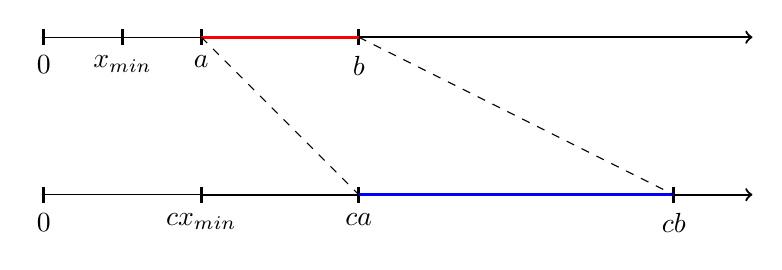
\begin{tikzpicture}
    % Draw number lines
    \draw[-] (0,2) -- (2,2);% node[right] {$x$};
    \draw[-] (0,0) -- (2,0);% node[right] {$cx$};
    \draw[->,thick] (2,2) -- (9,2);% node[right] {$x$};
    \draw[->,thick] (2,0) -- (9,0);% node[right] {$cx$};
    % Mark x and cx
    \draw[very thick] (1,2.1) -- (1,1.9) node[below] {$x_{min}$};
    \draw[very thick] (2,0.1) -- (2,-0.1) node[below] {$cx_{min}$};
    \draw[very thick] (0,2.1) -- (0,1.9) node[below] {$0$};
    \draw[very thick] (0,0.1) -- (0,-0.1) node[below] {$0$};
    \draw[very thick] (2,2.1) -- (2,1.9) node[below] {$a$};
    \draw[very thick] (4,0.1) -- (4,-0.1) node[below] {$ca$};
    \draw[very thick] (4,2.1) -- (4,1.9) node[below] {$b$};
    \draw[very thick] (8,0.1) -- (8,-0.1) node[below] {$cb$};
    % Interval on top line
    \draw[very thick,red] (2,2) -- (4,2);
    %\node[above,red] at (3,1.2) {Interval $I$};
    % Corresponding interval on bottom line
    \draw[very thick,blue] (4,0) -- (8,0);
    %\node[below,blue] at (6,-0.2) {Interval $cI$};
    % Dashed lines mapping intervals
    \draw[dashed] (2,2) -- (4,0);
    \draw[dashed] (4,2) -- (8,0);
\end{tikzpicture}
\end{center}
$^*$ Time permitting we can show this formally
\end{frame}

\begin{frame}
	\frametitle{Power laws}
    \color{gray}
    $$P(X>cx)=kP(X>x)\quad\bigstar$$
    \color{black}
    Consider:
    $$P(X>x)=Cx^{-\alpha},\quad i.e.\ P(X\leq x)=1-Cx^{-\alpha}$$
    Substituting into $\bigstar$ gives:
    \begin{eqnarray*}
        C(cx)^{-\alpha}&=&aC^{-\alpha}\\
        \Rightarrow c^{-\alpha}&=&a\\
        \Rightarrow -\alpha\log c&=&\log k\\
        \Rightarrow\alpha&=&-\frac{\log k}{\log c}
    \end{eqnarray*}
    So $P(X>x)=Cx^{-\alpha}$ is a solution. This gives:
    $$f_X(x)=\frac d{dx}\left(1-Cx^{-\alpha}\right)=\alpha Cx^{-\alpha}=Ax^{-\alpha}$$
    Observe: no value of $c$ can take us to $x=0$
\end{frame}

\begin{comment}
\begin{frame}
	\frametitle{Power laws}
    Let $X$ be a random variable describing distribution of wealth. We define: \par
    \begin{itemize}
        \item $N(x)$: total population with wealth at least $x$
        $$N(x)=N_{tot}P(X>x)=N_{tot}\int_x^{\infty}f(t)dt$$
        \item $W(x)$: total wealth in the population with wealth at least $x$
        $$W(x)=N(x)\int_x^{\infty}tf(t)dt$$
        \item $V(p)$: total wealth in the top proportion $p$ of the population
        $$V(p)=N(x_p)\int_{x_p}^{\infty}tf(t)dt,\quad\text{where}\ P(X>x_p)=p$$
        {\small\color{NavyBlue} - note that $x_p$ is defined implicitly in terms of $p$}
    \end{itemize}
    (Expressions for $N,W,V$ are included for completeness - you do not need to learn them)
\end{frame}
\end{comment}

\begin{frame}
	\frametitle{Power laws}
	{\bf\underline{Definition}}
    \begin{eqnarray*}
        p_X(k)&\propto& k^{-\gamma},\quad \gamma>1\\
        \text{OR}\quad f_Y(y)&\propto& y^{-\alpha},\quad \alpha>1
    \end{eqnarray*}
	{\small\color{NavyBlue} - the random variable is now the base of an exponent, not the power as in $exp(\lambda)$} \par
    Key observations:
    \begin{itemize}
        \item Multiplying $x$ by a constant $a$ decreases $f_X(x)$ by a factor of $a^{\alpha}$
        \item If $p_Y(y)=Ay^{-\alpha}$ then $\log p_Y(y)=\log A-\alpha\log y$ \par 
        - log both axes and you get a straight line!
    \end{itemize}
\end{frame}

\begin{frame}
	\frametitle{Power laws}
    \color{gray}
	{\bf\underline{Definition}}
    \begin{eqnarray*}
        p_X(k)&\propto& k^{-\gamma},\quad \gamma>1\\
        \text{OR}\quad f_Y(y)&\propto& y^{-\alpha},\quad \alpha>1
    \end{eqnarray*}
    \color{black}
	{\bf\underline{Questions}}
	\begin{itemize}
		\item Why do we need to specify $\gamma,\alpha>1$?
		\item What are the domain constraints in the discrete/continuous case?
        \item Exponential distributions and power laws look the same to the naked eye \par
        - how are they different?
	\end{itemize}
	%Consider the discrete case $X=1,2,\dots$ \par
\end{frame}

\begin{frame}
	\frametitle{Power laws}
	{\bf\underline{Definition}} \par
    The {\bf Pareto distribution} has parameters $\alpha$ and $x_{min}$ such that:
    $$f_X(x):=\left\{\begin{array}{lr}
			\frac{\alpha x_{min}}{x^{\alpha+1}}, & x\geq x_{min}\\
			0, & \text{otherwise}
		\end{array}\right.$$
    A Pareto distribution is a continuous, exact power law \par
    - in general, the term ``power law" applies in the limit $x\rightarrow\infty$ \par
    {\bf\underline{Mean}}
    $$f_X(x):=\frac{\alpha x_{min}}{\alpha-1},\quad\alpha>1$$
    {\bf\underline{Variance}}
    $$f_X(x):=\frac{\alpha x_{min}^2}{(\alpha-1)^2(\alpha-2)},\quad\alpha-2$$
    Exercise: derive these expressions \par
    Note: $\alpha$ is also the normalisation constant in the PDF
\end{frame}

\begin{frame}
	\frametitle{Power laws}
	\begin{columns}
		\column[b]{0.5\textwidth}
        \begin{center}
		\fbox{\includegraphics[width=\textwidth]{powerlawdiscrete.png}}
        Discrete power law ($x\geq 1)$)
        \end{center}
		\column[b]{0.5\textwidth}
        \begin{center}
		\fbox{\includegraphics[width=\textwidth]{powerlawcont.png}}
        Pareto distribution ($\alpha=1$)
        \end{center}
	\end{columns}
\end{frame}

\begin{comment}
\begin{frame}
	\frametitle{Power laws}
    {\bf\underline{Exercise}} \par
    Let $X$ follow a power law $f_X(x)=Ax^{-\alpha}$ for $x\geq x_{min}$. \par
    If we redefine the cutoff such that $x>10x_{min}$, show that the remaining outcomes are distributed according to the same power law \par
    Hint: use the formulation $P(X>x)=Cx^{-\alpha}$ \par
    Does this apply to other distributions? What about:
    \begin{itemize}
        \item The uniform distribution?
        \item The exponential distribution?
    \end{itemize}
    %``Scale invariance": the distribution still holds if we redefine the minimum value of $x$ \par
    %    - why can we not impose a maximum? \par
	%Crucial - same alpha!
\end{frame}
\end{comment}

\begin{frame}
	\frametitle{Power laws}
	{\bf\underline{Examples}} \par
	Magnitude/number of: 
	\begin{itemize}
		\item Income
		\item Solar flares
		\item Volcanic activity
		\item Academic citations
	\end{itemize}
	{\small\color{NavyBlue} - power laws typically describe the frequency of an ``amount of stuff"} \par
	%{\bf\underline{Exercise}} \par
	%Derive expressions for the mean and variance of a discrete power law with exponent $-\gamma$, $x=1,2,\dots$ \par 
	%Where appropriate, you may assume the normalisation factor of the PMF is $A_{\gamma}$
\end{frame}

\begin{frame}
	\frametitle{Example}
	The lifetime \( X \) (in hours) of a radioactive particle follows an exponential distribution:
\[
p(x) = \lambda e^{-\lambda x}, \quad x \geq 0
\]
where \( \lambda = 0.5 \) (i.e. a mean lifetime of 2 hours)
\begin{enumerate}[(a)]
    \item Compute \( E[X] \) and \( \text{Var}(X) \)
    \item Define a new variable \( Y = X^2 \), representing the square of the decay time. Compute \( E[Y] \) and \( \text{Var}(Y) \)
    \item Why does squaring increase the mean and variance? How does this transformation affect the shape of the distribution?
    \item In radioactive decay, if energy released is proportional to $X^2$, what does this transformation tell us about energy distributions in decay processes?
    \item Would it be reasonable to assume a power-law decay instead? Give a reason
\end{enumerate}

\end{frame}

%\begin{frame}
	%\frametitle{Warning}
    %Convergence
    %Need a lower cutoff $x_min>0$
    %alpha>1 for convergence
    %Time/stuff
    %Log one or both axs for a straight line - add to scale or scale to scale
%\end{frame}

%%%%%%%%%%%%%%%%%%%%%%%%%%%%%%%%%%%%%%%%%%%%%%%%%%%%%%%%%%%%%%%%
%%%%%%%%%%%%%%%%%%%%%%%%%%%%%%%%%%%%%%%%%%%%%%%%%%%%%%%%%%%%%%%%
\section{Week 7: sampling theory}
%Limit laws

%\begin{frame}
%	\frametitle{Sampling}
	%{\bf\underline{Examples}}
   %Real (data, finite), hypothetical (Poisson, infinite) \par
  %Sampling distribution of the mean \par  
%\end{frame}

\begin{frame}
	\frametitle{Sampling}
	Say you know $P(1<X<2)=0.9999$ \par
        Let $x$ be a value of $X$ \par
        - formally, $x$ is {\bf sampled} or simulation from the distribution of $X$ \par
        What can you say about $x$? \par
        \vspace{10pt}
        Aside: random number generation gives samples from $U(0,1)$ \par
        - how can I use this to sample from any known PDF?
        %x=F_U^{-1}(u)
\end{frame}

%\begin{frame}
%	\frametitle{Sampling}
%\end{frame}

\begin{frame}
		\frametitle{What is probability? (recap)}
		{\bf\underline{Frequestist interpretation}} \par
		Probability is the long-run relative frequency of an event occurring when an experiment is repeated under identical conditions:
		$$P(A)=\lim_{n\rightarrow\infty}\frac{k_n(A)}n$$
		where $k_n(A)$ denotes the observed number of occurences of $A$ in $n$ trials \par
		{\small\color{NavyBlue} - here is objective and based on observed data: each event has a true, fixed parameter defining its probability \par
			- the remainder of MATH163 will assume the frequentist interpretation of probability} \par
		{\bf\underline{Bayesian interpretation}} \par
		Probability represents a degree of belief or certainty about an event, updated as new evidence is observed. Recall:
		$$P(\theta\vert D)=\frac{P(D\vert\theta)P(\theta)}{P(D)}$$
		where $P(\theta\vert D)$ is the updated probability of a parameter $\theta$ given data $D$ \par
		{\small\color{NavyBlue} - you will still need to understand and use Bayes' rule in MATH163!}
\end{frame}

\begin{frame}
	\frametitle{Samples}
	{\bf\underline{Definitions}}
    \begin{itemize}
        \item {\bf i.d.d} means ``independent and identically distributed"
        \item If $X_1,X_2,\dots,X_n$ are i.d.d then they are $\lbrace X_1,X_2,\dots,X_n\rbrace$ is a {\bf random sample} of this distribution \par
        {\small\color{NavyBlue} - e.g. $X_i$ are successive rolls of a dice}
        \item After observation ($X_1=x_1,X_2=x_2,\dots,X_n=x_n$), the sequence $x_1,x_2,\dots,x_n$ is the {\bf sample data}
        \item In reality, the term {\bf sample} is used for random samples and sample data
        \item $\bar X_n:=\frac 1n\sum_{i=1}^nX_i$ - the mean of a sample of size $n$ \par
        {\bf - the subscript $n$ is always sample size}
    \end{itemize}
    Note: sampling without replacement means that successive samples are not independent
\end{frame}

\begin{frame}
	\frametitle{Sampling distributions}
	\begin{itemize}
		\item Collect a sample from a population (sample size $n$)
		\item Calculate the sample mean
		\item Repeat this process (with replacement), collecting a set of sample means
		\item These sample means will (probably) not be equal - they follow a distribution
		\item This distribution is the {\bf sampling distribution of the mean}
		\item Caveat: you need a big enough sample and a big enough population for this distribution to be interesting - why?
	\end{itemize}
%\end{frame}
%\begin{frame}
\begin{center}
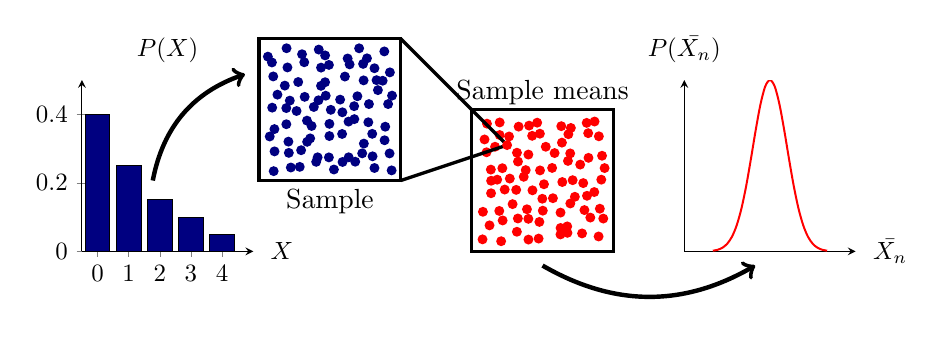
\begin{tikzpicture}[scale=0.9]
    % (a) Geometric distribution (First plot)
    \begin{scope}[shift={(0,0)}]
    \begin{axis}[
        at={(0,0)},
        anchor=south west,
        width=4cm, height=4cm,
        ybar,
        axis x line=middle,
        axis y line=left,
        xlabel style={at={(rel axis cs:1.05,0)}, anchor=west}, % Fix x-label position
        ylabel style={at={(rel axis cs:.5,1.05)}, anchor=south, rotate=-90},
        xmin=-.5, xmax=5,
        ymin=0, ymax=0.5,
        xlabel={$X$}, ylabel={$P(X)$},
        xtick={0,1,2,3,4},
    ]
    \addplot[fill=NavyBlue] coordinates {(0,0.4) (1,0.25) (2,0.15) (3,0.1) (4,0.05)};
    \end{axis}
    \end{scope}
    % (b) Circle with jittered blue dots
    \draw[very thick] (2.5,1) rectangle (4.5,3) node[midway, below, yshift=-25pt] {Sample};
;
    \foreach \x in {2.7,2.9,...,4.3} {
        \foreach \y in {1.2,1.4,...,2.8} {
            \fill[NavyBlue] (\x+rand*0.08,\y+rand*0.08) circle (2pt);
        }
    }
    % (c) Square with jittered blue dots
    \draw[very thick] (5.5,0) rectangle (7.5,2) node[midway, below, yshift=40pt] {Sample means};;
    \foreach \x in {5.7,5.9,...,7.3} {
        \foreach \y in {.2,.4,...,1.8} {
            \fill[red] (\x+rand*0.08,\y+rand*0.08) circle (2pt);
        }
    }
    \draw[very thick, black] (4.5,1) -- (6,1.5);
    \draw[very thick, black] (4.5,3) -- (6,1.5);
    \fill[red] (6,1.5) circle (2pt);
    \draw[ultra thick, black, ->, bend left] (1,1) to (2.3,2.5);
    \draw[ultra thick, black, ->, bend right] (6.5,-.2) to (9.5,-.2);
    % (d) Gaussian distribution
    \begin{scope}[shift={(8.5,0)}]
    \begin{axis}[
        anchor=south west,
        width=4cm, height=4cm,
        axis lines=middle,
        xlabel style={at={(axis description cs:1.05,0)}, anchor=west},
        ylabel style={at={(axis description cs:0,1.05)}, anchor=south},
        xlabel={$\bar{X_n}$}, ylabel={$P(\bar{X_n})$},
        xmin=1.5, xmax=4.5,
        ymin=0, ymax=1,
        xtick=\empty, ytick=\empty,
        domain=2:4
    ]
    \addplot[smooth,red,thick] {exp(-((x-3)^2)/(2*0.3^2))};
    \end{axis}
    \end{scope}
\end{tikzpicture}
\end{center}
\end{frame}

\begin{frame}
	\frametitle{Sampling distributions}
    {\bf Key idea: we can view the mean of a sample of size $n$ as a random variable} \par
    $\bar X_n$ denotes a random variable that follows the sampling distribution of the mean of $X$
    \begin{itemize}
        \item $n$ is the sample size
        \item $\mu$ is the population mean
        \item $\sigma^2$ is the population variance
    \end{itemize}
    {\bf\underline{Mean}}
    \begin{eqnarray*}
        E[\bar X_n]&=&E\left[\frac 1n\sum_{i=1}^nX_i\right]\\
        &=&\frac 1n\sum_{i=1}^nE[X_i]\quad\text{(linearity of expectation)}\\
        &=&\frac 1n \times nE[X_1]\quad\text{(i.d.d.)}\\
        &=&E[X_1]=\mu
    \end{eqnarray*}
    - the mean of the sampling distribution of the mean is equal to the population mean
    %Recall the laws of large numbers: \par
    %As sample size gets larger, the mean of the sample converges to the mean of the population \par
    %{\bf\underline{Corollary}} \par
    %The mean of the sampling distribution of the mean is equal to the population mean
\end{frame}

\begin{frame}
	\frametitle{Standard error}
	What is the variance of the sampling distribution of the mean?
	\begin{eqnarray*}
		Var(\bar X_n)&=&Var\left(\frac 1n\sum_{i=1}^nX_i\right)\\
		&=&\frac 1{n^2}\sum_{i=1}^nVar(X_i)\\
		&=&\frac 1{n^2}n\sigma^2=\frac{\sigma^2}n\\
		\text{standard error}\ \sigma_{\bar X}&=&\frac{\sigma}{\sqrt{n}}
	\end{eqnarray*}
	%Standard error of the mean is the standard deviation of the sampling distribution of the mean
\end{frame}

\begin{frame}
	\frametitle{The laws of large numbers}
	There are $2$ laws of large numbers, but they both intuitively mean the following: \par
	{\bf As sample size gets larger, the mean of the sample converges to the mean of the population} \par
        Formally, if $X_1,X_2,\dots,X_n$ are i.d.d with mean $\mu$ and variance $\sigma^2$ then:
        $$\bar X_n\xrightarrow{\text{$n\rightarrow\infty$}}\mu$$
\end{frame}

\begin{frame}
	\frametitle{The laws of large numbers}
	Let $X_1,X_2,\dots X_n$ be i.d.d with $E(X_1)=E(X_2)=\dots=E(X_n)=\mu$ \par
	%$$\bar X_n\rightarrow \mu\ \text{as}\ n\rightarrow\infty$$
	{\bf\underline{The weak law of large numbers} (WLLN):} \par
	$$\lim_{n\rightarrow\infty} P\left(\vert\bar X_n-\mu\vert<\epsilon\right)=1\quad\text{OR}\quad \lim_{n\rightarrow\infty}P\left(\vert\bar X_n-\mu\vert\geq\epsilon\right)=0$$
        {\bf\underline{Lemma} (Chebyshev's inequality)} \par
        If $X>0$ then, for any $\epsilon >0$ we have:
        $$P(X\geq\epsilon)\leq\frac{E[X^2]}{\epsilon^2}$$
        {\bf\underline{Proof of lemma}} \par
        Define the {\bf indicator function}:
        \begin{eqnarray*}
		\mathbf 1_{X\geq\epsilon} = \left\{\begin{array}{lr}
			1, & X\geq\epsilon\\
			0, & X<\epsilon
		\end{array}\right.\\
        \text{Then}\quad E[X^2]\geq E[X^2\mathbf 1_{X\geq\epsilon}]\geq E[\epsilon^2\mathbf 1_{X\geq\epsilon}]=\epsilon^2P(X\geq\epsilon)\quad\blacksquare
        \end{eqnarray*}
        %{\small\color{NavyBlue} - note that we are NOT interested in the limit $\epsilon\rightarrow 0$ here. In fact, this result is more relevant for large $\epsilon$}
\end{frame}

\begin{frame}
	\frametitle{The laws of large numbers}
        {\bf\underline{Proof of WLLN}} \par
        We will show that $\lim_{n\rightarrow\infty}P\left(\vert\bar X_n-\mu\vert\geq\epsilon\right)=0$:
        \begin{eqnarray*}
		E[(\bar X_n-\mu)^2]&=&Var(\bar X_n)\\
        &=&\frac{\sigma^2}n\\
        \Rightarrow P\left(\vert\bar X_n-\mu\vert\geq\epsilon\right)&\leq&\frac{E[(\bar X_n-\mu)^2]}{\epsilon^2}\quad\text{(using Chebyshev's inequality)}\\
        &=&\frac{\sigma^2}{n\epsilon^2}\xrightarrow{\text{$n\rightarrow\infty$}}0\quad\blacksquare
	\end{eqnarray*}
    {\small\color{NavyBlue} - note that the limit in question is $n\rightarrow\infty$, not $\epsilon\rightarrow 0$}
\end{frame}

\begin{comment}
\begin{frame}
	\frametitle{The laws of large numbers}
	Random variables can converge in numerous ways \par
        Let $\{X_1,X_2,\dots,X_n\}$ be a sequence of random variables \par
        $$X_n\xrightarrow{\text{?}}Y\ \text{as}\ n\rightarrow\infty$$
	\begin{itemize}
		\item Convergence in distribution (``$\xrightarrow{\text{$d$}}$") \par
		 - outcomes are increasingly well modeled by a given distribution
		\item Convergence in probability (``$\xrightarrow{\text{$p$}}$") \par
		- the probability of an “unusual” outcome becomes increasingly small
		\item ``Almost sure" convergence (``$\xrightarrow{\text{$a.s.$}}$") \par
		- events for which $X_n$ does not converge to $Y$ have probability $0$
	\end{itemize}
    We will not explore these in MATH163 - just be aware that convergence of random variables can happen in several ways
\end{frame}
\end{comment}

\begin{frame}
	\frametitle{The laws of large numbers}
	%Let $X_1,X_2,\dots X_n$ be i.d.d with $E(X_1)=E(X_2)=\dots=E(X_n)=\mu$
	%$$\bar X_n\rightarrow \mu\ \text{as}\ n\rightarrow\infty$$
        Recall $\bar X_n$ is the mean of $n$ i.d.d. random variables with $E[X_i]=\mu$ \par
	{\bf\underline{The weak law of large numbers} (WLLN):} \par
	$$\bar X_n\xrightarrow{\text{$p$}}\mu\ \text{as}\ n\rightarrow\infty\quad\text{i.e.}\ \lim_{n\rightarrow\infty} P\left(\vert\bar X_n-\mu\vert<\epsilon\right)=1$$
    - ``convergence in probability" \par
    {\small\color{NavyBlue} - a sequence of probabilities converges to zero} \par
	{\bf\underline{The strong law of large numbers} (SLLN:)} \par
        %If the $X_i$ also have finite variance, then:
        Under slightly stronger conditions, we have:
	$$\bar X_n\xrightarrow{\text{$a.s.$}} \mu\ \text{as}\ n\rightarrow\infty\quad\text{i.e.}\ P\left(\lim_{n\rightarrow\infty} \vert\bar X_n-\mu\vert<\epsilon\right)=1$$
    - ``almost sure convergence" \par
    %- but do we have convergence in distribution?
    {\small\color{NavyBlue} - this is a statement about the probability of a sequence converging to zero} \par
    {\bf As we approach this limit, there is still variation in sample means}
\end{frame}

\begin{frame}
    \frametitle{Approximate PMF}
    %Recall the frequentist definition of probability: \par
    %$P(a<X<b)=\alpha$ means as we take larger and larger samples, the proportion of values in the interval $[a,b]$ converges to $\alpha$ \par
    Let $X_1,X_2,\dots,X_n$ be i.i.d. with $p_X(k)=P(X_1=k)>0$. Then: \par
    {\bf\underline{Corollory of WLLN}} \par
    $$\frac 1n\sum_{i=1}^n\mathbf 1_{X_i=k}\xrightarrow{n\rightarrow\infty} E[\mathbf 1_{X_i=k}]=p_X(k)$$
    {\small\color{NavyBlue} - as samples get larger, relative frequency converges to probability mass} \par
    More precisely, $\forall\epsilon>0,n=1,2,\dots$, we have:
    $$P\left(\left|\frac 1n\sum_{i=1}^n\mathbf 1_{X_i=k}-p_X(k)\right|\geq\epsilon\right)\leq\frac{1}{4n\epsilon^2}\xrightarrow{n\rightarrow\infty}0$$
    {\bf\underline{Proof}}
    $$P\left(\left|\frac 1n\sum_{i=1}^n\mathbf 1_{X_i=k}-p_X(k)\right|\geq\epsilon\right)\leq\frac{Var(\mathbf 1_{X_1=k})}{n\epsilon^2}=\frac{p_X(k)(1-p_X(k))}{n\epsilon^2}\leq\frac{1}{4n\epsilon^2}$$
    (using that fact that $\mathbf 1_{X_i=k}\sim Bernouilli(p_X(k))$ ans $sup_{0\leq a\leq 1}a(1-a)=\frac 14$)
    %We can use R to see this
\end{frame}

\begin{frame}
    \frametitle{Approximate CDF}
    The same applies to PDFs (written out for completeness) \par
    Let $X_1,X_2,\dots,X_n$ be i.i.d. with $F_X(t)=P(X_1\leq t)>0$. Then: \par
    {\bf\underline{Corollory of WLLN}} \par
    $$\frac 1n\sum_{i=1}^n\mathbf 1_{X_i\leq t}\xrightarrow{n\rightarrow\infty} E[\mathbf 1_{X_i\leq t}]=F_X(t)$$
    More precisely, $\forall\epsilon>0,n=1,2,\dots$, we have:
    $$P\left(\left|\frac 1n\sum_{i=1}^n\mathbf 1_{X_i\leq t}-F_X(t)\right|\geq\epsilon\right)\leq\frac{1}{4n\epsilon^2}\xrightarrow{n\rightarrow\infty}0$$
    {\bf\underline{Proof}}
    $$P\left(\left|\frac 1n\sum_{i=1}^n\mathbf 1_{X_i\leq t}-F_X(t)\right|\geq\epsilon\right)\leq\frac{Var(\mathbf 1_{X_1\leq t})}{n\epsilon^2}=\frac{F_X(t)(1-F_X(t))}{n\epsilon^2}\leq\frac{1}{4n\epsilon^2}$$
    %(using that fact that $\mathbf 1_{X_i=k}\sim Bernouilli(p_X(k))$ ans $sup_{0\leq a\leq 1}a(1-a)=\frac 14$
    Recall the frequentist interpretation of statistics!
    %We can use R to see this
    %We can use R to see this
\end{frame}

\begin{frame}
    \frametitle{Example}
    Let \( X_1, X_2, \dots, X_n \) be independent random variables with \(X_i \sim \text{Geom}(p)\forall i\), i.e.:
\[
P(X_i = k) = (1 - p)^k p, \quad k = 0,1,2,3, \dots
\]
(a) Let \( \bar{X}_n = \frac{1}{n} \sum_{i=1}^{n} X_i \) be the sample mean. Using the WLLN, determine how large \( n \) must be so that 
\[
P(|\bar{X}_n - \mathbb{E}[X]| \geq 0.1) \leq 0.01
\]
\color{gray}
(b) For a fair coin (\( p = 0.5 \)), let \( X_1, X_2, \dots, X_n \) be i.i.d. geometric random variables, where \( X_i \) represents the number of failures before the first success. Set \( n = 100 \). Use the CLT to approximate:
\[
P(\bar{X}_n \geq \mathbb{E}[X] + 0.1)
\]
\color{black}
\end{frame}

\begin{frame}
	\frametitle{The central limit theorem (CLT)}
	{\bf CLT: if sample size $n$ is fixed across all samples and $\sigma^2<\infty$, \par
        then the sampling distribution of the mean is normal}
	\begin{itemize}
		\item Formally:
		\begin{eqnarray*}
			\bar X_n&\xrightarrow{\text{$d$}}&N(\mu, \sigma/\sqrt{n})\ \text{as}\ n\rightarrow\infty\\
			\text{OR}\ \frac{\bar X_n-\mu}{\sigma/\sqrt{n}}&\xrightarrow{\text{$d$}}&N(0,1)\ \text{as}\ n\rightarrow\infty
		\end{eqnarray*}
		where $\mu$ is the mean of $X$ and $\bar X_n$ and $\sigma$ is the s.d. of $X$
		%$\bar X\sim N(\mu, \sigma/\sqrt{n})$ in the limit as sample size $n\rightarrow\infty$
		\item Is this surprising? Is it obvious?
		%\item How can we put this to use?
		%\item This is the classical CLT: there are other (generalised) variants
		\item This is the classical CLT: there are other (generalised) variants \par
		{\small\color{NavyBlue} - we an account for sampling from non-identical distributions, or distributions with infinite variance}
	\end{itemize}
	%$^*$Conditions: sample size $n$ is fixed across all samples, and $\sigma^2<\infty$
\end{frame}

\begin{frame}
	\frametitle{The central limit theorem (CLT)}
	\centering
	\fbox{\includegraphics[width=.5\textwidth]{clt.jpg}}
\end{frame}

\begin{frame}
    \frametitle{Example}
    \color{gray}
    Let \( X_1, X_2, \dots, X_n \) be independent random variables with \(X_i \sim \text{Geom}(p)\forall i\), i.e.:
\[
P(X_i = k) = (1 - p)^k p, \quad k = 0,1,2,3, \dots
\]
(a) Let \( \bar{X}_n = \frac{1}{n} \sum_{i=1}^{n} X_i \) be the sample mean. Using the WLLN, determine how large \( n \) must be so that 
\[
P(|\bar{X}_n - \mathbb{E}[X]| \geq 0.1) \leq 0.01
\]
\color{black}
(b) For a fair coin (\( p = 0.5 \)), let \( X_1, X_2, \dots, X_n \) be i.i.d. geometric random variables, where \( X_i \) represents the number of failures before the first success. Set \( n = 100 \). Use the CLT to approximate:
\[
P\left( \bar{X} \geq \mathbb{E}[X] + 0.1 \right).
\]
\end{frame}

\begin{frame}
	\frametitle{The central limit theorem (CLT)}
	Why are so many variables (approximately) normally distributed? \par 
        Let \( X_1, X_2, \dots, X_n \) be independent random variables with means \( \mu_i \) and variances \( \sigma_i^2 \). Consider the normalized sum:
        \[
        S_n = \frac{1}{\sqrt{\sum_{i=1}^{n} \sigma_i^2}} \left( \sum_{i=1}^{n} (X_i - \mu_i) \right)
        \]
        Then the {\bf Generalised Central Limit Theorem (GCLT)} states:
        \[S_n\xrightarrow{\text{$d$}}N(0,1)\]
        assuming the Lindeberg condition is satisfied. \par
        The Lindeberg condition ensures that no individual variable has too large an impact on the sum. Formally, for each \( \epsilon > 0 \), it requires that:
        \[
        \frac{1}{\sum_{i=1}^{n} \sigma_i^2} \sum_{i=1}^{n} E\left[ (X_i - \mu_i)^2 \mathbf{1}_{|X_i - \mu_i| > \epsilon} \right] \to 0 \quad \text{as} \quad n \to \infty
        \]
\end{frame}

\begin{frame}
    \frametitle{The central limit theorem (CLT)}
    Which of the following variables do you expect are NOT normally distributed? Why?
    \begin{itemize}
        \item Human height
        \item Income in the UK
        \item IQ
        \item Exam scores in large class
        \item Time to failure of electronic devices
        \item Blood pressure
        \item Daily temperature in a city
        \item Shoe size in adult women
    \end{itemize}
\end{frame}

\begin{frame}
	\frametitle{Normal approximations}
	Recall the Bernoulli distribution $p_X(1)=1-p_X(0)=p$, \par
	What is the sampling distribution of the mean?$$\bar x=\frac 1n\sum_{i=1}^n$$
	Consider the {\it sum} of $n$ Bernoulli trials: $S_n=\sum_{i=1}^nX_i$ \par
	We have:
	$$P(S_n=k)={n\choose k} p^k(1-p)^{1-k}$$
	- this is binomial! \par
	By the CLT:
        $$S_n\xrightarrow{\text{$d$}} N(np,np(1-p))\ \text{as}\ n\rightarrow\infty$$
	{\small\color{NavyBlue} - we have used the fact that the sum of $n$ Bernoulli random variables is binomial to show that the normal distribution can approximate the binomial distribution for large $n$}
\end{frame}

\begin{frame}
	\frametitle{Estimators}
	%Question: how can we use properties of a sample (statistics) to approximate properties of the population (parameters)? \par
        {\bf\underline{Definition}} \par
        An {\bf statistic} is any function of a random sample $X_1,X_2,\dots,X_n$ \par
        A {\bf parameter} $\theta$ is a property of the population the sample is drawn from \par
        An {\bf estimator} $\hat\theta$ is a function of statistics used to estimate $\theta$ \par
	Example: we typically estimate population mean $\mu$ with sample mean $\bar X$\par
	{\small\color{NavyBlue} - this seems obvious, but from the CLT we know $\bar X$ has non-zero variance, so there is uncertainty in the estimate} \par
	What about estimating variance?
	$S_0^2:=\frac 1n\sum_i(X_i-\mu)^2$ \par
	{\small\color{NavyBlue} - here we use each point in the sample to estimate the population variance \par
		- note that we are using $\mu$, the population mean} \par
	What if we also need to estimate $\mu$? \par Consider $S_0^2:=\frac 1n\sum_i(X_i-\bar X)^2$
\end{frame}

%\if{handout}{
	\begin{frame}
		\frametitle{Estimators}
		Recall: $E[aX]=aE[X],\ E[XY]=E[X]E[Y]$ IF $X$ and $Y$ are independent \par
		Also, $\sigma^2=E[X^2]-\mu^2\Rightarrow E[X^2]=\sigma^2+\mu^2$
		{\tiny
			\begin{eqnarray*}
				E[S_0^2]&=&E\left[\frac 1n\sum_{i=1}^n\left(X_i-\frac 1n\sum_{j=1}^nX_j\right)^2\right] \\
				&=&\sum_{i=1}^n\frac 1nE\left[X_i^2-\frac 2nX_i\sum_{j=1}^nX_j+\frac 1{n^2}\sum_{j=1}^nX_j\sum_{k=1}^nX_k\right] \\
				&=&\frac 1n\sum_{i=1}^n\left(E[X_i^2]-\frac 2n\left(\sum_{j\neq i}E[X_iX_j]+E[X_i^2]\right)+\frac 1{n^2}\sum_j\sum_{k\neq j}E[X_jX_k]+\frac 1{n^2}\sum_jE[X_j^2]\right) \\
				&=&\frac 1n\sum_{i=1}^n\left(\frac{n-1}nE[X_i^2]-\frac 2n\sum_{j\neq i}E[X_iX_j]+\frac 1{n^2}\sum_j\sum_{k\neq j}E[X_jX_k]\right) \\
				&=&\frac 1n\sum_{i=1}^n\left(\frac{n-1}n(\sigma^2+\mu^2)-\frac 2n(n-1)\mu^2+\frac 1{n^2}n(n-1)\mu^2\right) \\
                &=&\frac 1n\sum_{i=1}^n\frac{n-1}n\sigma^2 \\
				&=&\frac{n-1}n\sigma^2 
			\end{eqnarray*}
		}
		So $S_0^2$ will always underestimate $\sigma^2$ - why?
	\end{frame}
	%}

\begin{frame}
	\frametitle{Estimators}
	Recall: $S_0^2:=\frac 1n\sum_i(X_i-\bar X)^2$ and $E[S_0^2]=\frac{n-1}n\sigma^2$ \par
	This is an example of a {\bf biased estimator} \par
	{\bf\underline{Definitions}} \par
	Let $\hat\theta$ be an estimator of a parameter $\theta$. Then:
	\begin{itemize}
		\item $\hat\theta$ is {\bf unbiased} if $E[\hat\theta]=\theta$
		\item $\hat\theta$ is {\bf consistent} if $\lim_{n\rightarrow\infty}P(\vert\hat\theta-\theta\vert\geq\epsilon)=0\ \forall\epsilon>0$
	\end{itemize}
	The sample mean $\bar X$ is an unbiased, consistent estimator of $\mu$ \par
	The quantity $S_0^2$ is a biased but consistent estimator of $\sigma^2$ \par
	Can you construct an unbiased estimator of $\sigma^2$?
	\begin{center}
		\fbox{\includegraphics[width=.2\textwidth]{countdown.jpg}}
	\end{center}
\end{frame}

%	\begin{frame}
%		\frametitle{Estimators}
%		Recall: standard error $\sigma_{\bar X}=\sigma/\sqrt n$ is the s.d. of the sampling distribution of the mean \par
%		What if we don't know the value of $\sigma$?
%	\end{frame}

\begin{frame}
	\frametitle{Estimators}
	{\bf\underline{Definition}} \par
	$$\text{Sample variance}\ S^2:=\frac 1{n-1}\sum_i(X_i-\bar X)^2$$%\boxed
	%Cochran's theorem applied to variance - chi squared distribution with n-1 dof
\end{frame}

\begin{frame}
	\frametitle{Notation}
	From now on, let $X_1,X_2,\dots,X_n$ be i.d.d. random variables, i.e. a sample (with replacement) of size $n$ \par
	{\small\color{NavyBlue} - each $x$ corresponds to a single measurement of something, and a collection of these things form a sample. For example, each $X$ is the outcome of a coin toss, dice roll, height, temperature etc} \par
	Then we define:
	\begin{itemize}
		\item $\mu$: population mean
		\item $\bar X$: sample mean
		\item $\sigma$: population s.d.
		\item $\sigma_X=S=\sqrt{\frac 1{n-1}\sum_i(X_i-\bar X)^2}$: sample s.d.
		\item $\sigma_{\bar X}=\sigma/\sqrt n$: standard error
		\item $\hat\sigma_{\bar X}=S/\sqrt n$: estimate of standard error using sample s.d. \par
		{\small\color{NavyBlue} - annoyingly this doesn't have a distinct name and is often referred to as ``standard error"}
	\end{itemize}
\end{frame}

%%%%%%%%%%%%%%%%%%%%%%%%%%%%%%%%%%%%%%%%%%%%%%%%%%%%%%%%%%%%%%%%
%%%%%%%%%%%%%%%%%%%%%%%%%%%%%%%%%%%%%%%%%%%%%%%%%%%%%%%%%%%%%%%%
\section{Week 8: statistical testing I}

\begin{frame}
	\frametitle{Statistical testing}
	When we collect data, we sample from a population. There are several questions we can ask about a sample or samples:
	\begin{itemize}
		\item Has my sample come from the population I think it has come from?%Is my sample representative of the population? \\
		%OR has my sample come from the population I think it has come from?\\
		\item Have these $2$ samples come from the same population or not?
		\item Can I tell from my sample if this population follows the distribution I think it follows?
	\end{itemize}
\end{frame}

\begin{comment}
\begin{frame}
	\frametitle{$z$-test}
	Question: has my sample come from the population I think it has come from?
	\begin{itemize}
		\item Test the mean of the sample $\bar X_n$ against the hypothesized population mean $\mu_0$ \par
		%{\small\color{NavyBlue} - example: is this dice biased? \par
		\item Consider the following case:
		\begin{itemize}
			\item Large sample size ($n\geq 30$) so the CLT is manifest \par
            OR sampling from a normal distribution
			\item Or population variance $\sigma^2$ is known
            
		\end{itemize}
		\item Then the sample mean is a single draw from the sampling distribution of the mean, and we can calculate the probability of a sample mean being at least this far from $\mu_0$
	\end{itemize}
\end{frame}
\end{comment}

\begin{frame}
	\frametitle{$z$-test}
	Testing the mean of the sample $\bar X_n$ against the hypothesized population mean $\mu_0$:
    \begin{table}[h]
    \centering
    \begin{tabular}{|c|c|c|c|l|}
        \hline
        \textbf{Sample Size} & \textbf{Population Normal?} & \textbf{Variance Known?} & \textbf{Test to Use} \\% & \textbf{Reason} \\ 
        \hline
        \( n < 30 \) & $\checkmark$ & $\checkmark$ & \( z \)-test \\% & Sample mean follows normal distribution \\ 
        \( n < 30 \) & $\checkmark$ & $\times$  & \( t \)-test \\% & Must estimate variance, use \( t \)-distribution \\ 
        \( n < 30 \) & $\times$  & $\checkmark$ & Neither$^*$ \\% (use nonparametric test) & Sample mean may not be normal \\ 
        \( n < 30 \) & $\times$  & $\times$  & Neither$^*$ \\% (use nonparametric test) & Same issue as above \\ 
        \( n > 30 \) & $\checkmark$ & $\checkmark$ & \( z \)-test \\% & Large \( n \) ensures normality \\ 
        \( n > 30 \) & $\checkmark$ & $\times$  & \( t \)-test \\% & Large \( n \) ensures normality, estimate variance \\ 
        \( n > 30 \) & $\times$  & $\checkmark$ & \( z \)-test \\% & CLT ensures approximate normality \\ 
        \( n > 30 \) & $\times$  & $\times$  & \( t \)-test \\% CLT ensures approximate normality, estimate variance \\ 
        \hline
    \end{tabular}
    %\caption{Choosing between \( Z \)-tests, \( t \)-tests, and nonparametric tests}
    %\label{tab:zt_tests}
\end{table}
$^*$Use nonparametric test (not covered in MATH163)
\end{frame}

\begin{frame}
	\frametitle{$\bigstar$ $z$-test}
	A $z$-test is performed as follows:
	\begin{enumerate}
		\item State your null hypothesis, e.g. $H_0:\ E[\bar X_n]=\mu_0$ \par
		{\small\color{NavyBlue} - the sample mean and the mean of the conjectured population are the same}
		\item State your alternate hypothesis, e.g. $H_1:\ E[\bar X]\neq\mu_0$ \par
		{\small\color{NavyBlue} - this is the negation of $H_0$ - it includes {\it anything} not consistent with $H_0$}
		\item State your significance level (as a percentage): $100\alpha\%$\par
		{\small\color{NavyBlue} - if only $100\alpha\%$ of sample means lie further away from $\mu$ than $\bar x$, then we reject $H_0$ in favour of $H_1$}
		\item Calculate the sample mean $\bar x$ and the ``$z$-score" $z=\frac{\bar x-\mu_0}{\sigma/\sqrt n}$ \par
		{\small\color{NavyBlue} - here $\bar x$ denotes our specific sample mean, and $\bar X_n$ the random variable describing sample means \par
			%- sample means follow a normal distribution, and $z$ is the ``standardised" equivalent, i.e. linearly transformed to a normal distribution with mean $0$ and s.d. $1$ \par
			- recall that, if $\bar X_n\sim N(\mu_0,\sigma)$, we have $\frac{\bar X_n-\mu_0}{\sigma/\sqrt n}\sim N(0,1)$}%. We convert to a standard normal distribution in order to numerically evaluate probabilities}
		\item Calculate the $z$-score $z^*$ associated with your significance level \par
            OR the $p$-value associated with the $z$-score from your sample mean
		%{\small\color{NavyBlue} - c.f. next slide ``(one tail or two?")}
		%\item If $H_0$ is true, what is the probability that a sample mean is at least as far from the population mean as $\bar x$?
		\item Do we reject $H_0$?
	\end{enumerate}
\end{frame}

\begin{frame}
	\frametitle{$z$-test: one tail or two?}
	\begin{columns}
		\column{0.5\textwidth}
		\centering
		\fbox{\includegraphics[width=\textwidth]{normal1tail.png}}
		Standard normal distribution: $z_{0.95}=1.645,\ z_{0.05}=-1.645$
		\column{0.5\textwidth}
		\centering
		\fbox{\includegraphics[width=\textwidth]{normal2tail.png}}
		Standard normal distribution: $z_{0.975}=1.96,\ z_{0.025}=1.96$
	\end{columns}
	%{\bf\underline{Example}} \par
	%$5\%$ significance level:
	One tail test: does $\bar x$ lie within the least likely $100\alpha\%$ of values according to $H_0$ \par
	{\small\color{NavyBlue} - is there evidence for a change in the parameter $\mu$?} \par
	$\bar x$ lies within the least likely $100\alpha\%$ large or small of values according to $H_0$ \par
    {\small\color{NavyBlue} - is there evidence for an increase/decrease in $\mu$?} \par
    {\bf The wording of your null hypothesis determines which test to use}
\end{frame}

\begin{frame}
    \frametitle{$z$-scores}
    Question: What is the value $z^*$ such that $P(Z<z^*)=\alpha$ \par
    Answer: The value at which the CDF $F_Z(z)=\alpha$, so $z^*=F_Z^{-1}(\alpha)$ \par
    - you have to look it up in a table (old-fashioned), use a calculator (1980s/exam), or use R (obvs) \begin{itemize}
    \item One-tail test: calculate inverse normal CDF of EITHER $\alpha$ OR $1-\alpha$, depending which ``side" of the normal distribution you need
    \item Two-tail test: calculate the inverse normal CDF of $\frac{\alpha}2$ AND $1-\frac{\alpha}2$
    \end{itemize}
    Terminology:
    \begin{itemize}
    \item The {\bf rejection region} is the set of values of $z$ such that we reject $H_0$
    \item The $p$-value associated with $z$ is the probability of a sample mean lying at least as far away from $\mu_0$ as $z$ - $p<\alpha\Rightarrow$ reject $H_0$: \par
    $p=P(Z>|z|)$ (one tail) OR $p=2P(Z>|z|)$ (two-tail) \par
    {\bf Quoting a $p$-value is an alternate way of presenting a hypothesis test}
    \end{itemize}
\end{frame}

\begin{frame}
    \frametitle{Hypothesis testing}
    Warnings:
    \begin{itemize}
        \item We never ``accept" $H_0$ or $H_1$ \par- we only ever ``reject" or ``fail to reject"
        \item {\bf Type I error:} incorrectly rejecting $H_0$ when it is true \par
        - false positive
        \item {\bf Type II error:} incorrectly failing to reject $H_0$ when it is false \par
        - false negative
        \item Smaller significance levels reduce the risk of type I errors but increase he risk of type II errors
    \end{itemize}
\end{frame}

\begin{frame}{$z$-test: example 1}
    Scenario: \par
    A hospital claims that the average recovery time for patients undergoing a specific surgery is $8$ days. A researcher suspects that the average recovery time may differ from this value. The researcher collects data from a sample of $5$0 patients and finds an average recovery time of $7.5$ days. Assume that the population standard deviation $\sigma$ is known to be $2$ days. \par
    
    Perform $z$-test at the $5\%$ significance level to determine if the actual mean recovery time differs significantly from $8$ days.
\end{frame}

\begin{frame}{$z$-test: example 1}
    Scenario: \par
    A hospital claims that the average recovery time for patients undergoing a specific surgery is $8$ days. A researcher suspects that the average recovery time may differ from this value. The researcher collects data from a sample of $5$0 patients and finds an average recovery time of $7.5$ days. Assume that the population standard deviation $\sigma$ is known to be $2$ days. \par
    
    Perform $z$-test at the $5\%$ significance level to determine if the actual mean recovery time differs significantly from $8$ days. \par
    We have:
    \begin{itemize}
        \item Null Hypothesis: The mean recovery time is $8$ days ($H_0:\mu=8$)
        \item Alternate Hypothesis: The mean recovery time is not $8$ days ($H_1:\mu\neq 8$)
        \item This is a two-tail test because the researcher suspects the recovery time could be either shorter or longer than 8 days
        \item $\bar x=7.5, \mu_0=8,\ \sigma=2,\ n=50$. This gives us:
        $$z=\frac{\bar x-\mu_0}{\sigma/\sqrt n}=\frac{7.5-8}{2/\sqrt 50}\approx -1.77$$
    \end{itemize}
\end{frame}

\begin{frame}{$z$-test: example 1}
    We have:
    \begin{itemize}
        \item Null Hypothesis: The mean recovery time is $8$ days ($H_0:\mu=8$)
        \item Alternate Hypothesis: The mean recovery time is not $8$ days ($H_1:\mu\neq 8$)
        \item This is a two-tail test because the researcher suspects the recovery time could be either shorter or longer than 8 days
        \item $\bar x=7.5, \mu_0=8,\ \sigma=2,\ n=50$. This gives us:
        $$z=\frac{\bar x-\mu_0}{\sigma/\sqrt n}=\frac{7.5-8}{2/\sqrt 50}\approx -1.77$$
    \end{itemize}
    Option 1:
    \begin{itemize}
        \item $z^*_{0.025}=F_Z^{-1}(0.025)=-1.96<-1.77$ (R function ``qnorm(0.025)") \par
        Note: here we fail to reject $H_0$ if $z\in[-z^*,z^*]$
    \end{itemize}
    Option 2:
    \begin{itemize}
        \item $p=2P(Z<-1.77)=2P(Z>1.77)=0.0768>0.05$
    \end{itemize}
    Conclusion: we fail to reject $H_0$
\end{frame}

\begin{frame}{$z$-test: example 2}
Scenario: \par
A climate research institute reports that the average number of hurricanes in a particular region is historically $12$ per year, with a known population standard deviation $\sigma=3$. A researcher suspects that recent climate changes have increased the frequency of hurricanes. To test this hypothesis, they collect data for a recent sample of $36$ years, finding an average of $13.5$ hurricanes per year. \par
Perform a $z$-test at the $5\%$ significance level to determine if the recent average frequency of hurricanes is significantly higher than the historical average.
\end{frame}

\begin{frame}{$z$-test: example 2}
Scenario: \par
A climate research institute reports that the average number of hurricanes in a particular region is historically $12$ per year, with a known population standard deviation $\sigma=3$. A researcher suspects that recent climate changes have increased the frequency of hurricanes. To test this hypothesis, they collect data for a recent sample of $36$ years, finding an average of $13.5$ hurricanes per year. \par
Perform a $z$-test at the $5\%$ significance level to determine if the recent average frequency of hurricanes is significantly higher than the historical average. \par
We have:
    \begin{itemize}
        \item Null Hypothesis: The mean number of hurricanes per year is {\bf at most} $12$ ($H_0:\mu\leq 12$)
        \item Alternate Hypothesis: The mean recovery time is more than $12$ ($H_1:\mu>12$)
        \item This is a one-tail test because we only care if $\mu$ is larger than expected
        \item $\bar x=13.5, \mu_0=12,\ \sigma=3,\ n=36$. This gives us:
        $$z=\frac{\bar x-\mu_0}{\sigma/\sqrt n}=\frac{13.5-12}{3/\sqrt 36}=3$$
    \end{itemize}
\end{frame}

\begin{frame}{$z$-test: example 2}
We have:
    \begin{itemize}
        \item Null Hypothesis: The mean number of hurricanes per year is $12$ ($H_0:\mu=12$)
        \item Alternate Hypothesis: The mean recovery time is more than $12$ ($H_1:\mu>8$)
        \item This is a one-tail test because we only care if $\mu$ is larger than expected
        \item $\bar x=13.5, \mu_0=12,\ \sigma=3,\ n=36$. This gives us:
        $$z=\frac{\bar x-\mu_0}{\sigma/\sqrt n}=\frac{13.5-12}{3/\sqrt 36}=3$$
    \end{itemize}
    Option 1:
    \begin{itemize}
        \item $z^*_{0.05}=F_Z^{-1}(0.05)=1.64<3$ (R function ``qnorm(0.05)")
        Note: here we fail to reject $H_0$ if $z<z^*$
    \end{itemize}
    Option 2:
    \begin{itemize}
        \item $p=P(Z>3)=P(Z<-3)=0.00135<0.05$
    \end{itemize}
    Conclusion: we reject $H_0$
\end{frame}

\begin{frame}
	\frametitle{$z$-test}
        Warnings:
        \begin{itemize}
            \item $z$-tests require known, finite varince and large sample sizes
            \item EITHER compare probabilities ($p$-value and significance level) OR $z-$scores (standardized sample mean and $\pm z_{\alpha}$ or $\pm z_{\alpha/2}$) \par
        \end{itemize}
	BUT what if the sample size is small, or the population variance unknown?
	\begin{itemize}
		\item Small sample size: CLT hasn't ``kicked in"
		\item Population variance unknown: we need to use the sample variance to approximate it
	\end{itemize}
    %In these cases, we need a $t$-test instead \par
    There are ways of dealing with this, but we need to introduce some other key concepts first
\end{frame}

\begin{frame}
	\frametitle{Confidence intervals}
	In a $z$-test, the normal distribution is centered on $\mu_0$, and we check if $\bar x$ is within a given distance of $\mu_0$
    \begin{itemize}
        \item The normal distribution is centered on $\mu_0$, the {\it hypothesized} mean of the sampling distribution
        \item We calculate the probability that a sample mean $\bar X_n$ is at least $|\bar X_n-\mu_0|$ away from $\mu_0$ ($p$-values)
        \item This process is used to evaluate our hypothesis regarding $\mu_0$
    \end{itemize}
    Now consider the following: we are using $\bar X_n$ to estimate $\mu$, the {\it true} population mean
    \begin{itemize}
        \item Construct a (symmetric) interval around $\bar x$ such that a sample mean lies in this interval with probability $1-\alpha$
        \item Centre this interval around $\bar x$
        \item There is now a probability $1-\alpha$ that this new interval contains the mean $\mu$
        \item Constructing the interval requires only knowledge of the variance
        \item $100(1-\alpha)\%$ is known as the {it confidence level}
    \end{itemize}
\end{frame}

\begin{frame}
		\frametitle{What is probability? (recap)}
		{\bf\underline{Frequestist interpretation}} \par
		Probability is the long-run relative frequency of an event occurring when an experiment is repeated under identical conditions:
		$$P(A)=\lim_{n\rightarrow\infty}\frac{k_n(A)}n$$
		where $k_n(A)$ denotes the observed number of occurences of $A$ in $n$ trials \par
		{\small\color{NavyBlue} - here is objective and based on observed data: each event has a true, fixed parameter defining its probability \par
			- ther remainder of MATH163 will assume the frequentist interpretation of probability} \par
		{\bf\underline{Bayesian interpretation}} \par
		Probability represents a degree of belief or certainty about an event, updated as new evidence is observed. Recall:
		$$P(\theta\vert D)=\frac{P(D\vert\theta)P(\theta)}{P(D)}$$
		where $P(\theta\vert D)$ is the updated probability of a parameter $\theta$ given data $D$ \par
		{\small\color{NavyBlue} - you will still need to understand and use Bayes' rule in MATH163!}
\end{frame}

\begin{frame}
\frametitle{Confidence intervals}
\begin{center}
    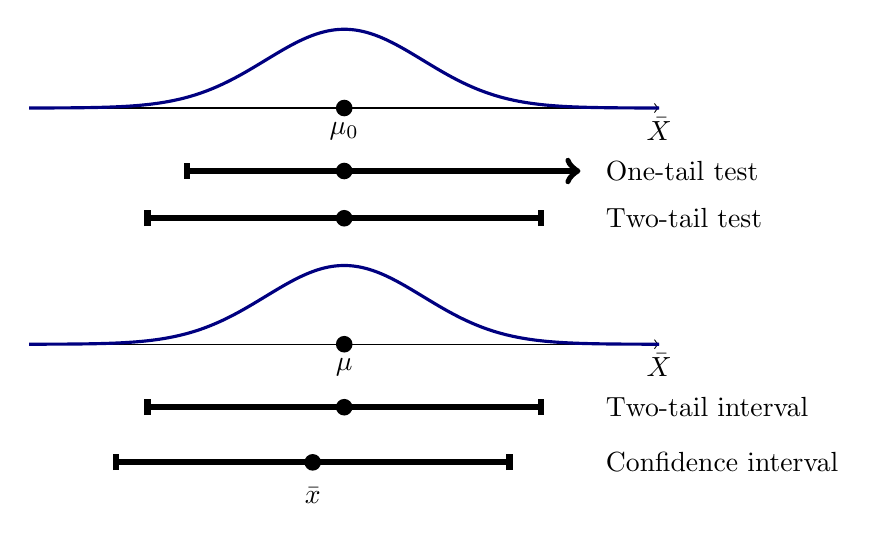
\begin{tikzpicture}
    % First normal distribution
    % Draw the x-axis and label it as $\bar{X}$
    \draw[->] (-4,0) -- (4,0) node[anchor=north] {$\bar{X}$};

    % Draw the normal distribution curve
    \draw[line width=.4mm, color=NavyBlue, domain=-4:4, smooth, samples=100] 
        plot (\x, {exp(-0.5*\x*\x)});

    % Label the mean, $\mu_0$
    \draw[thick] (0,0.05) -- (0,-0.05) node[anchor=north] {$\mu_0$};
    \fill (0,0) circle (3pt); % Larger filled circle at the center

    % One-sided 95% confidence interval
    \draw[->, line width=.8mm] (-2, -0.8) -- (3, -0.8); % Thicker horizontal arrow for 1-sided interval
    \draw[line width=.8mm] (-2, -0.9) -- (-2, -0.7); % Thicker vertical line at 5%
    \fill (0, -0.8) circle (3pt); % Larger circle at the middle of the CI aligned with $\mu_0$
    \node[anchor=west] at (3.2, -0.8) {One-tail test}; % Label for one-sided test

    % Two-sided 95% confidence interval
    \draw[line width=.8mm] (-2.5, -1.4) -- (2.5, -1.4); % Thicker horizontal line for 2-sided interval
    \draw[line width=.8mm] (-2.5, -1.5) -- (-2.5, -1.3); % Thicker vertical line at 2.5%
    \draw[line width=.8mm] (2.5, -1.5) -- (2.5, -1.3); % Thicker vertical line at 97.5%
    \fill (0, -1.4) circle (3pt); % Larger circle at the middle of the CI aligned with $\mu_0$
    \node[anchor=west] at (3.2, -1.4) {Two-tail test}; % Label for two-sided test

    % Second normal distribution (below the first)
    % Shifted downwards
    \begin{scope}[shift={(0,-3)}]
        % Draw the x-axis and label it as $\bar{X}$
        \draw[->] (-4,0) -- (4,0) node[anchor=north] {$\bar{X}$};

        % Draw the normal distribution curve
        \draw[line width=.4mm, color=NavyBlue, domain=-4:4, smooth, samples=100] 
            plot (\x, {exp(-0.5*\x*\x)});

        % Label the mean, $\mu$
        \draw[thick] (0,0.05) -- (0,-0.05) node[anchor=north] {$\mu$};
        \fill (0,0) circle (3pt); % Larger filled circle at the center

        % Two-sided 95% confidence interval
        \draw[line width=.8mm] (-2.5, -0.8) -- (2.5, -0.8); % Thicker horizontal line for 2-sided interval
        \draw[line width=.8mm] (-2.5, -0.9) -- (-2.5, -0.7); % Thicker vertical line at 2.5%
        \draw[line width=.8mm] (2.5, -0.9) -- (2.5, -0.7); % Thicker vertical line at 97.5%
        \fill (0, -0.8) circle (3pt); % Larger circle at the middle of the CI aligned with $\mu$
        \node[anchor=west] at (3.2, -0.8) {Two-tail interval}; % Label for 95% CI %(3.2, -0.8)

        % Repeated confidence interval shifted 10% to the left
        \draw[line width=.8mm] (-2.9, -1.5) -- (2.1, -1.5); % Thicker horizontal line, shifted left by 0.4 units
        \draw[line width=.8mm] (-2.9, -1.6) -- (-2.9, -1.4); % Thicker vertical line at left end
        \draw[line width=.8mm] (2.1, -1.6) -- (2.1, -1.4); % Thicker vertical line at right end
        \fill (-0.4, -1.5) circle (3pt); % Larger circle at the middle, shifted left
        \node[anchor=north] at (-0.4, -1.7) {$\bar{x}$}; % Label for the dot
        \node[anchor=west] at (3.2, -1.5) {Confidence interval}; % Label for 95% CI 
    \end{scope}
\end{tikzpicture}
\end{center}
\begin{itemize}
    \item $\mu_0$ is a {\it hypothesized} mean - ``does my sample mean lie in this interval?"
    \item $\mu$ is the true mean, but is {\it unknown}
    \item Variance $\sigma^2<\infty$ known and sample size large
\end{itemize}
\end{frame}

\begin{frame}
	\frametitle{Confidence intervals}
        By definition, we have:
        $$P\left(\mu-z_{\alpha/2}\frac{\sigma}{\sqrt n}<\bar x <\mu+z_{\alpha/2}\frac{\sigma}{\sqrt n}\right)=1-\alpha$$
        By symmetry, the interval
        $$CI_{\alpha}=\left(\bar x-z_{\alpha/2}\frac{\sigma}{\sqrt n},\bar x+z_{\alpha/2}\frac{\sigma}{\sqrt n}\right)$$
        contains $\mu$ with probability $1-\alpha$
     \par
     {\bf Warning: do not make probabalistic statements about $\mu$}, e.g. ``there is a $95\%$ chance that $\mu$ lies..." \par
     Interpretation: if we construct this interval around all possible sample means, then a proportion $\alpha$ of them will contain $\mu$ \par
\end{frame}

\begin{frame}
	\frametitle{Confidence intervals: example}
    A company is evaluating the effectiveness of two different advertising campaigns, Campaign A and Campaign B, in increasing product sales. They collect sales data from two large, independent regions where each campaign was run. The results are as follows:

\begin{itemize}
    \item Campaign A: Sample size $n_1 = 200$, sample mean $\bar{x}_1 = 520$, population standard deviation $\sigma_1 = 50$
    \item Campaign B: Sample size $n_2 = 250$, sample mean $\bar{x}_2 = 500$, population standard deviation $\sigma_2 = 60$
\end{itemize}

(a) Construct a 95\% confidence interval for the mean sales of Campaign A  \\
(b) Construct a 95\% confidence interval for the mean sales of Campaign B  \\
(c) Based on your confidence intervals from (a) and (b), determine whether there is evidence of a significant difference in mean sales between the two campaigns. Explain your reasoning.    
\end{frame}

\begin{frame}
	\frametitle{Confidence intervals: example}
    (a) The formula for a CI when the population standard deviation is known is:
\[
CI_{\alpha} = \bar{x} \pm z_{\alpha/2} \times \frac{\sigma}{\sqrt{n}}
\]
For a 95\% confidence level, $Z_{\alpha/2} = 1.96$.

\[
CI_A = 520 \pm 1.96 \times \frac{50}{\sqrt{200}} = 520 \pm 1.96 \times 3.54 = 520 \pm 6.94 = (513.06, 526.94)
\]

(b) Similarly, we calculate:

\[
CI_B = 500 \pm 1.96 \times \frac{60}{\sqrt{250}} = 500 \pm 1.96 \times 3.80 = 500 \pm 7.45 = (492.55, 507.45)
\]

(c) The confidence interval for Campaign A is $(513.06, 526.94)$, and for Campaign B it is $(492.55, 507.45)$. Since these intervals do not overlap, there is statistical evidence suggesting a significant difference in mean sales between the two campaigns at the 95\% confidence level
  
\end{frame}

\begin{frame}
	\frametitle{Confidence intervals}
Warning: so far, we have only considered cases where the $z$-test is appropriate \par
In practice, the population variance is usually unknown, so we must estimate it from the sample \par
— these are called ``nuisance parameters" \par
When the variance is unknown, the $t$-distribution is often required to account for the additional uncertainty in estimation \par
In the MATH163 exam, you will be told which test to use \par
- but you will have to justify the choice of test
\end{frame}

%%%%%%%%%%%%%%%%%%%%%%%%%%%%%%%%%%%%%%%%%%%%%%%%%%%%%%%%%%%%%%%%
%%%%%%%%%%%%%%%%%%%%%%%%%%%%%%%%%%%%%%%%%%%%%%%%%%%%%%%%%%%%%%%%

\section{Week 9: statistical testing II}

\begin{frame}
	\frametitle{Comparing distributions}
    $z$-tests: we compare a sample mean against a population mean \par
    More generally, we compare an estimator with a parameter \par
    What if instead we compare distributions? \par
    Consider discrete data (categorical or numeric) \par
    Note: this approach can be used with continuous data, but we need to ``bin" it first \par
    %- you will not be asked to do this in MATH163 \par 
    {\bf Question: was my sample drawn from the distribution I think it was drawn from?} \par
    {\ bf Goodnees of fit test: does my hypothesized distribution ``fit" the sample}
\end{frame}

\begin{frame}
	\frametitle{Example 1}
    We roll a dice 60 times. Outcomes are tracked in the table below
\begin{center}
    \begin{tabular}{r|cccccc}
        Outcome $i$ & 1 & 2 & 3 & 4 & 5 & 6 \\ \hline
        Frequency & 8 & 10 & 12 & 9 & 0 & 21 \\
    \end{tabular}
\end{center}
Is this a fair dice? \par
If it were then the {\bf expected frequencies} would be:
\begin{center}
    \begin{tabular}{r|cccccc}
        Outcome $i$ & 1 & 2 & 3 & 4 & 5 & 6 \\ \hline
        Frequency & 10 & 10 & 10 & 10 & 10 & 10 \\
    \end{tabular}
\end{center}
$H_0$: the dice is fair \par
$H_1$: the dice is not fair \par
Can we compute a single test statistic measuring deviation from expectation?
\end{frame}

\begin{frame}
	\frametitle{Example 1}
    In MATH163 we will only consider finite discrete distributions \par
    Yet $Y$ be a discrete finite random variable
    Label the outcomes $1,2,\dots,k$ and define $p_i=P(Y=i),\ i=1,2,\dots,k$ so that $\sum_{i=1}^kp_i=1$ \par
    Let $Y_1,Y_2,\dots,Y_n$ be i.i.d. random variables following the distribution of $Y$ \par
    Let $c_i$ be the frequency of each outcome measured in our data \par
    From the WLLN, we expect:
    $$\frac {c_i}n\approx p_i\quad\forall i$$
    i.e. $c_i-p_in\approx 0$ \par
    {\bf\underline{Definition}} \par
    The ``chi-squared statistic" is defined as:
    $$\mathcal{X}^2:=\sum_{i=1}^k\frac{(c_i-np_i)^2}{np_i}=n\sum_{i=1}^k\frac{\left(\frac{c_i}n-p_i\right)^2}{p_i}$$
\end{frame}

\begin{frame}
	\frametitle{General case}
    {\bf\underline{Theorem}} \par
    If our data $c_i$ are sampled from i.i.d random variables $Y_1,Y_2,\dots,Y_n$ then:
    \begin{eqnarray*}
        \mathcal{X}^2\xrightarrow{d}\chi^2_{k-1}\quad\text{as}\quad n\rightarrow\infty
    \end{eqnarray*}
    Where:
    $$\chi^2_{k-1}\sim\sum_{i=1}^{k-1}Z_i^2,\quad Z_i\sim N(0,1)\ \forall i$$
\end{frame}

\begin{frame}
	\frametitle{General case}
    Aside: for each $i$, we could the indicator function $\mathbf 1_{K-i}$ and apply the CLT to the binomial distribution $Bin(n,p_i)$, i.e.:
    $$z^2=\frac{(c_i-np_i)^2}{np_i(1-p_i)}$$
    {\bf - but this ignores the frequencies of the other outcomes!} \par
    %- the frequencies depend on each other \par
    The $\mathcal{X}^2$ statistic retains information about the {\bf distribution of data} \par
    Observe that the denominator is {\bf not} variance:
    $$\mathcal{X}^2:=\sum_{i=1}^k\frac{(c_i-np_i)^2}{np_i}$$
    - the $\mathcal{X}^2$ statistic uses a Poisson approximation to a multinomial distribution (not covered in MATH163)
    %- variance measures distance from the mean \par
    %- $\mathcal{X}^2$ measures distance between counts and expected counts under $H_0$
\end{frame}

\begin{frame}
	\frametitle{$\chi^2$ test}
    We perform a $\chi^2$ test by first choosing a significance level $\alpha\in(0,1)$ \par
    Next we compute $\mathcal{X}^2$, and $X\sim\chi^2_{n-1}$ \par
    Option 1: \par
    Compute $x=\chi^2_{k-1,\alpha}$ such that $P(X\geq x)=\alpha$ \par
    and reject $H_0$ if $x<\mathcal{X}^2$ \par
    Option 2: \par
    $p=P(X\geq\mathcal{X}^2)$ and reject $H_0$ if $p<\alpha$ \par
    %- the probability of the scaled sum of squared deviations being at least $\chi^2$ {\bf under} $H_0$
    %- this is the $p$-value approach in a $\chi^2$ test \par
    %Just like the $z$-test, we set a significance level $100\alpha\%$ and reject $H_0$ if $p<\alpha$ \par
    Note: smaller $p$ corresponds to a larger sum of scaled square deviations from expected outcomes under $H_0$ \par
    \begin{itemize}
        \item The {\bf rejection region} is $[\chi^2_{k-1,\alpha},\infty)$
        \item the {\bf $p$-value} is $P(X\geq\mathcal{X}^2)$
    \end{itemize}
\end{frame}

\begin{frame}
	\frametitle{$\chi^2$ distribution}
	\begin{columns}
		\column{0.5\textwidth}
		\centering
		\fbox{\includegraphics[width=\textwidth]{chi2.png}}
		$\chi^2$ distribution PDF
		\column{0.5\textwidth}
		\centering
		\fbox{\includegraphics[width=\textwidth]{chi2rejection.png}}
        Rejection region at 5\% significance level ($\chi^2_5$)
	\end{columns}
\end{frame}

\begin{frame}
	\frametitle{Example 1}
    Recall the potentially biased dice:
\begin{center}
    \begin{tabular}{r|cccccc}
        Outcome $i$ & 1 & 2 & 3 & 4 & 5 & 6 \\ \hline
        Frequency $O_i$ & 8 & 10 & 12 & 9 & 0 & 21 \\
        Expectation $E_i$ & 10 & 10 & 10 & 10 & 10 & 10 \\
    \end{tabular}
\end{center}
\[ \chi^2 = \sum_{i=1}^k \frac{(O_i - E_i)^2}{E_i} \]
Substituting values:
\begin{align*}
    \mathcal{X}^2 &= \frac{(8 - 10)^2}{10} + \frac{(10 - 10)^2}{10} + \frac{(12 - 10)^2}{10} + \frac{(9 - 10)^2}{10} + \frac{(0-10)^2}{10} + \frac{(21 - 10)^2}{10} \\
    &= \frac{4}{10} + 0 + \frac{4}{10} + \frac{1}{10} + \frac{100}{10} + \frac{121}{10} \\
    &= 0.4 + 0 + 0.4 + 0.1 + 10 + 12.1 \\
    &= 23
\end{align*}
If $X\sim\chi^2_{5}$ then $P(X>14)=0.01561<0.05$ and so we reject $H_0$ a the 5\% significance level
\end{frame}

\begin{frame}
	\frametitle{Warning}
    We need large enough sample sized for this approach to be valid:
    $$np_i\geq 5\quad\forall i$$
    Otherwise we have $2$ options:
    \begin{itemize}
        \item Add more data
        \item Combine outcomes
    \end{itemize}
\end{frame}

\begin{frame}
	\frametitle{Degrees of freedom}
    {\bf\underline{Question}} \par
    Why with $k$ outcomes is $\mathcal{X}^2$ distributed like a sum of $k-1$ squares of standard normal variables? \par
    Second application: testing for independence \par
    {\bf Test of independence: are these $2$ categorical variables independent within a population?}
\end{frame}

\begin{frame}
	\frametitle{Example 2}
    We want to test if there is an association between gender (male/female) and preference for a new product (like/dislike)
	\begin{center}
		\begin{tabular}{ c | c  c | c }
			& Like & Dislike & Total \\ \hline
			Female & 50 & 20 & 70 \\ %\hline
			Male & 40 & 30 & 70 \\ \hline
			Total & 90 & 50 & 140
		\end{tabular} 
	\end{center}%\par 
	Note the following:
	\begin{itemize}
		\item The data is partitioned by $2$ different variables (rows and columns)
		\item $H_0:$ Gender and preference are independent, i.e. $P(L|F)=P(L|M)=P(L)$
		\item We {\it could} have more rows (samples) or columns (outcomes)
	\end{itemize}
	{\bf\underline{Questions}} \par
	\begin{itemize}
		\item What is $H_1$?
		\item How many degrees of freedom do we have?
        \item Do we have enough evidence to reject $H_0$ at the 5\% significance level?
	\end{itemize}
\end{frame}

\begin{frame}
	\frametitle{Example 2}
    {\bf\underline{Answers}} \par
    $H_1$: Gender and preference are not independent
    \begin{columns}
		\column{0.5\textwidth}
		\centering
			\begin{tabular}{ c | c  c | c }
				& Like & Dislike & Total \\ \hline
				Female & 50$^{(1)}$ & 20$^{(2)}$ & 70 \\ %\hline
				Male & 40$^{(3)}$ & 30$^{(4)}$ & 70 \\ \hline
				Total & 90 & 50 & 140
			\end{tabular}
			\vspace{5pt}
			Original table
		\column{0.5\textwidth}
		\centering
		\begin{tabular}{ c | c  c | c }
			& Like & Dislike & Total \\ \hline
			Female & 45$^{(1)}$ & 25$^{(2)}$ & 70 \\ %\hline
			Male & 45$^{(3)}$ & 25$^{(4)}$ & 70 \\ \hline
			Total & 90 & 50 & 140
		\end{tabular}
		\vspace{5pt}
		Expected values under $H_0$
	\end{columns}
    Our data gives is the row and column sums - so we only have 1 degree of freedom! \par
    Note that $n$ does not feature explicitly in the $\mathcal{X}^2$ statistic
\end{frame}

\begin{frame}
	\frametitle{Example 2}
    Compute the $\mathcal{X}^2$ statistic:
    \begin{eqnarray*}
        \mathcal{X}^2&=&\frac{(50-45)^2}{45}+\frac{(20-25)^2}{25}+\frac{(40-45)^2}{45}+\frac{(30-25)^2}{25}\\
        &=&\frac{25}{45}+\frac{25}{25}+\frac{25}{45}+\frac{25}{25}\\
        &=&3.111
    \end{eqnarray*}
    This gives $p=0.146$, so we do not reject $H_0$ at the 5\% significance level
\end{frame}

\begin{frame}
	\frametitle{$2\times 2$ tables: the quick way}
    Given the following \(2 \times 2\) contingency table:
\[
\begin{array}{c|cc|c}
  & \text{Category 1} & \text{Category 2} & \text{Row Total} \\
  \hline
  \text{Group 1} & a & b & a + b \\
  \text{Group 2} & c & d & c + d \\
  \hline
  \text{Column Total} & a + c & b + d & N
\end{array}
\]
Under the null hypothesis, the expected values for each cell are calculated as:
\[
E_{ij} = \frac{(\text{row total}) \times (\text{column total})}{N}
\]
Thus, the expected frequencies are:
\[
E_{11} = \frac{(a+b)(a+c)}{N}, \quad
E_{12} = \frac{(a+b)(b+d)}{N}
\]
\[
E_{21} = \frac{(c+d)(a+c)}{N}, \quad
E_{22} = \frac{(c+d)(b+d)}{N}
\]
This gives:
$$\chi^2 = \frac{N(ad - bc)^2}{(a + b)(c + d)(a + c)(b + d)}$$
\end{frame}

\begin{frame}
	\frametitle{Degrees of freedom}
    When we have an $m\times n$ table of frequencies, how many degrees of freedom do we have?
    \begin{center}
    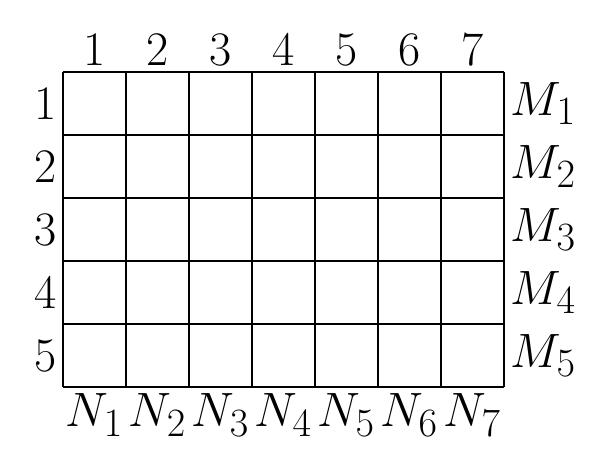
\begin{tikzpicture}[scale=0.8]  % Scale down by 80%
        % Define table size
        \def\nrow{5}  % Total rows
        \def\ncol{7}  % Total columns
        % Draw table grid lines on top
        \foreach \x in {0,...,\ncol} {
            \draw[thick] (\x,0) -- (\x,\nrow);
        }
        \foreach \y in {0,...,\nrow} {
            \draw[thick] (0,\y) -- (\ncol,\y);
        }
        % Labels for row sums (smaller text)
        \foreach \y in {1,...,\nrow} {
            \node[right,scale=0.7] at (\ncol,\nrow-\y+0.5) {\Huge $M_{\y}$};
        }
        % Labels for column sums (below table, smaller text)
        \foreach \x in {1,...,\ncol} {
            \node[below,scale=0.7] at (\x-0.5,0) {\Huge $N_{\x}$};
        }
        % Table numbering (row numbers on the left, smaller text)
        \foreach \y in {1,...,\nrow} {
            \node[left,scale=0.7] at (0,\nrow-\y+0.5) {\Huge \y};
        }
        % Column numbering (above table, smaller text)
        \foreach \x in {1,...,\ncol} {
            \node[above,scale=0.7] at (\x-0.5,\nrow) {\Huge \x};
        }
    \end{tikzpicture}
    \end{center}
    
\end{frame}

\begin{frame}
	\frametitle{Degrees of freedom}
    When we have an $m\times n$ table of frequencies, how many degrees of freedom do we have?
\begin{center}
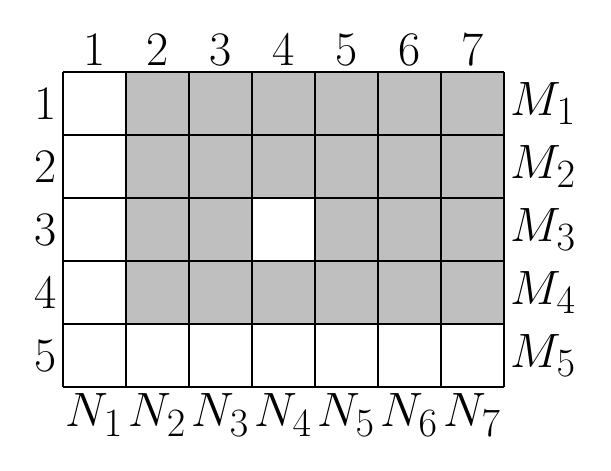
\begin{tikzpicture}[scale=0.8]  % Scale down by 80%
    % Define table size
    \def\nrow{5}  % Total rows
    \def\ncol{7}  % Total columns
    % Shade the (nrow-1) x (ncol-1) area (first 4 rows and 6 columns)
    \foreach \x in {1,...,6} {
        \foreach \y in {1,...,4} {
            \fill[gray!50] (\x,\y) rectangle ++(1,1);
        }
    }
    % Highlight one specific cell darker
    \fill[white] (3,2) rectangle ++(1,1);
    % Draw table grid lines on top
    \foreach \x in {0,...,\ncol} {
        \draw[thick] (\x,0) -- (\x,\nrow);
    }
    \foreach \y in {0,...,\nrow} {
        \draw[thick] (0,\y) -- (\ncol,\y);
    }
    % Labels for row sums (smaller text)
    \foreach \y in {1,...,\nrow} {
        \node[right,scale=0.7] at (\ncol,\nrow-\y+0.5) {\Huge $M_{\y}$};
    }
    % Labels for column sums (below table, smaller text)
    \foreach \x in {1,...,\ncol} {
        \node[below,scale=0.7] at (\x-0.5,0) {\Huge $N_{\x}$};
    }
    % Table numbering (row numbers on the left, smaller text)
    \foreach \y in {1,...,\nrow} {
        \node[left,scale=0.7] at (0,\nrow-\y+0.5) {\Huge \y};
    }
    % Column numbering (above table, smaller text)
    \foreach \x in {1,...,\ncol} {
        \node[above,scale=0.7] at (\x-0.5,\nrow) {\Huge \x};
    }
\end{tikzpicture}
\end{center}
Our data gives the row and column totals, so we have $(m-1)\times(n-1)$ degrees of freedom \par
This only applies when $m,n>1$ - why? \par... and there's more
\end{frame}

\begin{frame}
	\frametitle{Example 3}
    A study is conducted to examine the growth of bulbs planted in different locations. A total of 370 gardeners each plant 4 bulbs and record how many successfully sprout after 3 weeks. The observed results are:
    \begin{center}
        \begin{tabular}{r|ccccc}
            Number of bulbs sprouted & 0 & 1 & 2 & 3 & 4 \\ \hline
            Frequency & 12 & 54 & 107 & 130 & 67 \\
        \end{tabular}
    \end{center}
It is assumed that these results follow a binomial distribution $Bin(4,p)$ for some probability 
$p$, which is estimated using the overall proportion of bulbs that sprouted \par
Perform a $\chi^2$ goodness of fit test to assess whether the binomial model provides a suitable fit for the data the 5\% significance level \par
Note: this is a goodness of fit test
\end{frame}

\begin{frame}
	\frametitle{Example 3}
    {\bf\underline{Answer}} \par
    $H_0$: $X\sim Bin(4,p)$, $H_1$: $X\nsim Bin(n,p)$ \par
    Note: we have not made a hypothesis about $p$ - we need to estimate it from the data! \par
    Since each gardener plants 4 bulbs, the total number of planted bulbs is $370 \times 4 = 1480$ zpar
    The total number of successful sprouts is $(0 \times 12) + (1 \times 54) + (2 \times 107) + (3 \times 130) + (4 \times 67) = 926$ \par
    The estimated probability of sprouting is therefore $\hat p=\frac{926}{1480} \approx 0.626$ \par
    The expected frequencies are given by $E_k = 370 \times P(X = k)$:
    \begin{center}
        \begin{tabular}{r|ccccc}
            Number of bulbs sprouted & 0 & 1 & 2 & 3 & 4 \\ \hline
            Frequency $O_i$ & 12 & 54 & 107 & 130 & 67 \\
            Expected frequency $E_i$ & 7.24 & 48.47 & 121.69 & 135.79 & 56.82 \\
        \end{tabular}
    \end{center}
    This gives:
    \begin{eqnarray*}
        \chi^2 &=& \frac{(12 - 7.24)^2}{7.24} + \frac{(54 - 48.47)^2}{48.47} + \frac{(107 - 121.69)^2}{121.69} + \frac{(130 - 135.79)^2}{135.79} + \frac{(67 - 56.8)^2}{56.8}\\
        &\approx& 7.605
    \end{eqnarray*}
\end{frame}

\begin{frame}
    \frametitle{Degrees of freedom}
    %{\bf\underline{Answer}} \par
    Recall that the use of sample mean to compute sample variance reduces the effective sample size by $1$ \par- this is the loss of a degree of freedom \par
    If we have $n$ categories, then:
    \[
    df = n - 1 - \text{(number of estimated parameters)}
    \]
    If we have an $m\times n$ table then:
    \[
    df = (m-1)(n-1) - \text{(number of estimated parameters)}
    \]
\end{frame}

\begin{frame}
    \frametitle{Example 3}
    %\bf\underline{Answer}} \par
    Here $n=5$, so:
    \[
    df = n - 1 - \text{(number of estimated parameters)}
    \]
    The critical value for \( \alpha = 0.05 \) and \( df = 3 \) is approximately $7.815$ \par
    Since \( \chi^2 = 7.605 < 7.815 \), we fail to reject \( H_0 \) at the 5\% significance level \par
    This suggests that the binomial assumption is reasonable \par
    The critical value for \( \alpha = 0.1 \) and \( df = 3 \) is approximately $6.251$ \par
    - so we would reject $H_0$ at the 10\% significance level
\end{frame}

\begin{frame}
    \frametitle{$\chi^2$ test: summary}
    \begin{enumerate}
    \item State $H_0$ and $H_1$
    \item Complete the following table:
    \begin{center}
    \begin{tabular}{ r || c | c | c | c | c | c | c|}
    Value $i$ & 0 & 1 & 2 & 3 & 4 & ...\\ \hline
    $O_i$ &  &  &  &  &  &  \\ \hline
    $E_i$ &  &  &  &  &  &  \\ \hline
    $O_i-E_i$ &  &  &  &  &  &  \\ \hline
    $(O_i-E_i)^2$ &  &  &  &  &  &  \\ \hline
    $(O_i-E_i)^2/E_i$ &  &  &  &  &  &  \\ \hline
    \end{tabular}
    \end{center}
    \item compute $\mathcal{X}^2=\sum_{i=1}^k(O_i-E_i)^2/E_i$
    \item Compute the degrees of freedom: \par
    $1$ variable: $df = n - 1 -$ (number of estimated parameters) \par
    $2$ variables: $df = (m-1)(n-1) -$ (number of estimated parameters) \par
    \item Compute the value $x$ such that $P(X\geq x)=\alpha$, where $X\sim\chi^2_{df}$ \par
    OR compute the $p$-value of $\mathcal{X}^2$, i.e. $P(X\geq \mathcal{X}^2)$
    \item Decide whether to reject $H_0$ at significance level $100\alpha\%$
\end{enumerate}
\end{frame}

\begin{frame}
    \frametitle{Example 4}
    {\bf Test of homogeneity: is the distribution of a categorical variable independent of another attribute across different groups} \par 
    A hospital network is evaluating the effectiveness of a new treatment across three hospitals. Each hospital administers the same treatment, and doctors record whether the treatment was successful or unsuccessful. The observed data is:
\[
\begin{array}{c|cc|c}
\text{Hospital} & \text{Success} & \text{Failure} & \text{Total Patients} \\
\hline
\text{A} & 42 & 18 & 60 \\
\text{B} & 70 & 30 & 100 \\
\text{C} & 56 & 34 & 90 \\
\hline
\text{Total} & 168 & 82 & 250
\end{array}
\]
We assume that the treatment has an underlying probability of success \( p \) that is the same for all hospitals \par
Perform a chi-squared goodness-of-fit test at th 5\% significance level to determine whether the observed success rates significantly differ from the expected rates under the null hypothesis \par
\end{frame}

\begin{comment}
\begin{frame}
	\frametitle{Comparing distributions}
	What if we don't know the distribution we are sampling from? \par
	We may hypothesis for this distribution, i.e. $H_0: P(Y=i)=q_i$ \par
	{\small\color{NavyBlue} - Example: is this dice biased? If the dice is unbiased, we have $p_i=\frac 1k \forall k$} \par%, i.e. we know the $p_i$'s
	Recall CLT $\implies\frac{\frac{c_i}{n}-p_i}{p_i}\sim N(0,1)$, where $p_i$ is the true value \par
	Define $\mathcal{X}^2:=\sum_{i=1}^k\left[\frac{c_i-nq_i}{nq_i}\right]^2=n\sum_{i=1}^k\left[\frac{\frac{c_i}{n}-q_i}{q_i}\right]^2$ \par
	{\small\color{NavyBlue} - the notation ``squared" just indicates that this quantity is necessarily positive} \par
	{\bf IF $q_i=p_i\ \forall i$ THEN $\frac{\chi^2}n$ is sampled from a sum of squares of $k-1$ normal distributions}
\end{frame}

\begin{frame}
	\frametitle{The $\chi^2$ distribution}
	{\bf\underline{Definition}} 
	\begin{eqnarray*}
		Y\sim\chi^2_k\ \iff\ Y&=&\sum_{i=1}^kZ_i^2,\ Z_i\sim N(0,1)\\
		f_Y(y)&=&\frac 1{2^{\frac k2}\Gamma(\frac k2)}y^{\frac k2-1}e^{-\frac x2}
	\end{eqnarray*}
	We say $Y$ follows a $\chi^2$ distribution with $k$ degrees of freedom \par
	{\small\color{NavyBlue} - you will not need to use this explicit PDF in MATH163 - the important thing to understand is that $\chi^2$ random variables are sums of squares of standard normal random variables} \par
\end{frame}

\begin{frame}
	\frametitle{Comparing distributions}
	{\bf\underline{Example 1}} \par
	We want to test if there is an association between gender (male/female) and preference for a new product (like/dislike)
	\begin{center}
		\begin{tabular}{ c | c  c | c }
			& Like & Dislike & Total \\ \hline
			Female & 50 & 20 & 70 \\ %\hline
			Male & 40 & 30 & 70 \\ \hline
			Total & 90 & 50 & 140
		\end{tabular} 
	\end{center}%\par 
	Note the following:
	\begin{itemize}
		\item There is $1$ sample split into $4$ groups
		\item ``Like/dislike" is the outcome variable
		\item $H_0:$ Gender and preference are independent, i.e. $P(L|F)=P(L|M)=P(L)$
		\item We {\it could} have more rows (samples) or columns (outcomes)
	\end{itemize}
	Questions:
	\begin{itemize}
		\item What is $H_1$?
		\item If $H_0$ is true, then which quantities are sampled from a normal distribution (by the CLT)? Which distribution are they sampled from?
	\end{itemize}
\end{frame}

\begin{frame}
	\frametitle{Comparing distributions}
	{\bf\underline{Example 1}} \par
	{\color{black!40}
		We want to test if there is an association between gender (male/female) and preference for a new product (like/dislike)
		\begin{center}
			\begin{tabular}{ c | c  c | c }
				& Like & Dislike & Total \\ \hline
				Female & 50 & 20 & 70 \\ %\hline
				Male & 40 & 30 & 70 \\ \hline
				Total & 90 & 50 & 140
			\end{tabular} 
		\end{center}%\par 
	}
	Answers:
	\begin{itemize}
		\item $H_1:$ gender and preference are independent
		\item Each statistic (F/L, F/D, M/L, M/D) is a sample mean from a binomial distribution (``success"=``like" or ``dislike") \par
		- to see this, we consider the expected outcomes under $H_0$
	\end{itemize}
\end{frame}

\begin{frame}
	\frametitle{Comparing distributions}
	{\bf\underline{Example}} \par
	If $H_0$ is true, what are the expected counts in each row/column? \par 
	\begin{itemize}
		\item $P(L),P(D)=$ column total$/$grand total 
		\item $P(F),P(M)=$ row total/grand total
		\item $P(L\cap F)=P(L|F)P(L)=P(F)P(L)$ \par
		$\qquad\qquad\ =$ column total$\times$row total$/$(grand total)$^2$
		\item $E[X_{L,F}]=$ column total$\times$row total$/$grand total
	\end{itemize}
	\vspace{5pt}
	\begin{columns}
		\column{0.5\textwidth}
		\centering
		{\color{black!40}
			\begin{tabular}{ c | c  c | c }
				& Like & Dislike & Total \\ \hline
				Female & 50$^{(1)}$ & 20$^{(2)}$ & 70 \\ %\hline
				Male & 40$^{(3)}$ & 30$^{(4)}$ & 70 \\ \hline
				Total & 90 & 50 & 140
			\end{tabular}
			\vspace{5pt}
			Original table
		}
		\column{0.5\textwidth}
		\centering
		\begin{tabular}{ c | c  c | c }
			& Like & Dislike & Total \\ \hline
			Female & 45$^{(1)}$ & 25$^{(2)}$ & 70 \\ %\hline
			Male & 45$^{(3)}$ & 25$^{(4)}$ & 70 \\ \hline
			Total & 90 & 50 & 140
		\end{tabular}
		\vspace{5pt}
		Expected values under $H_0$
	\end{columns}
	%Question: how can we formally compare these tables? \par 
	For convenience, the $4$ compartments are indexed $1,2,3,4$. Let $\bar x_i$ denote the data observed value in compartment $i$, and $E[X_i]$ the expected value under $H_0$
\end{frame}

\begin{frame}
	\frametitle{Comparing distributions}
	{\bf\underline{Example}} \par
	\begin{columns}
		\column{0.5\textwidth}
		\centering
		{\color{black!40}
			\begin{tabular}{ c | c  c | c }
				& Like & Dislike & Total \\ \hline
				Female & 50$^{(1)}$ & 20$^{(2)}$ & 70 \\ %\hline
				Male & 40$^{(3)}$ & 30$^{(4)}$ & 70 \\ \hline
				Total & 90 & 50 & 140
			\end{tabular}
			\vspace{5pt}
			Original table
		}
		\column{0.5\textwidth}
		\centering
		\begin{tabular}{ c | c  c | c }
			& Like & Dislike & Total \\ \hline
			Female & 45$^{(1)}$ & 25$^{(2)}$ & 70 \\ %\hline
			Male & 45$^{(3)}$ & 25$^{(4)}$ & 70 \\ \hline
			Total & 90 & 50 & 140
		\end{tabular}
		\vspace{5pt}
		Expected values under $H_0$
	\end{columns}
	%Question: how can we formally compare these tables? \par
	%Answer: 
	Each of the $4$ tabulated data values $x_i$ is a sample mean from a binomial distribution with sample size $n=140$ and $p_i=\frac{E[X_i]}{n}$ \par
	%{\small\color{NavyBlue} - e.g. if $p_1=P(L\cap F)=\frac{45}{140}$ (under $H_0$) then $1-p_1=P(\neg (L\cap F))=P(D\cup M)$, and each individual in the sample is a female who likes the product with probability $p_1$. This is a Bernoulli distribution with $\mu=p_1$} \par 
	We have:
	$$\bar X_i\sim Bin(E[X_i],n)\xrightarrow{\text{$p$}}N(E[X_i],np_i(1-p_i))\ \text{as}\ n\rightarrow\infty$$
	{\small\color{NavyBlue} - recall that the sampling distribution of the sum of Bernoulli distributions is binomial, and the CLT gives us normal approximation} \par
	%{\bf Just like variance measures deviation from the mean, we measure the deviation of out observations from the expectation under $H_0$} \par 
	%Let $X_i,\ i=1,2,3,4$ denote the table entries, and let $n=140$
	%$$\text{Consider}\quad z^2_i:=\left(\frac{\bar x_i-E[X_i]}{\sigma_{\bar X}}\right)^2=\frac{(\bar x_i-np_i)^2}{np_i(1-p_i)}$$
        {\bf BUT, if we know one entry in the table then we can work out all of the others, since we know the row and column sums} \par
        {\small\color{NavyBlue} - the $\bar X_i$ are not independent}
\end{frame}


%	\begin{frame}
%		\frametitle{Comparing distributions}
%		{\bf\underline{Example}} \par
%		{\color{black!40}
%			{\bf Just like variance measures deviation from the mean, we measure the deviation of out observations from the expectation under $H_0$} \par
%			$$\text{Consider}\quad z^2_i:=\left(\frac{\bar x_i-E[X_i]}{\sigma_{\bar X}}\right)^2=\frac{(\bar x_i-np_i)^2}{np_i(1-p_i)}$$
%		}
%		This is the square of a binomial random variable which, by the CLT, is well approximated by the square of a standard normal random variable \par
%		{\small\color{NavyBlue} - recall normal approximation to binomial}\par
%		BUT the $z_i$ are not independent - why?
%	\end{frame}


\begin{frame}
	\frametitle{Comparing distributions}
	%{\bf\underline{Example}} \par
	%{\bf Just like variance measures deviation from the mean, we measure the deviation of out observations from the expectation under $H_0$}
	{\bf How can we measure the deviation of out observations from the expectation under $H_0$?}
	\begin{eqnarray*}
		\text{Consider}\quad y_i:&=&\frac{\bar x_i-E[X_i]}{\sigma_{\bar X}}\\
            &=&\frac{\bar x_i-np_i}{\sqrt{np_i(1-p_i)}}
	\end{eqnarray*}
	- we could perform a $z$-test just one of the data points%, but this would ignore the distribution of the others \par
\end{frame}

%	\begin{frame}
%		\frametitle{Comparing distributions}
%		{\bf\underline{Example}} \par
%		{\color{black!40}
%			{\bf Just like variance measures deviation from the mean, we measure the deviation of out observations from the expectation under $H_0$} \par
%			$$\text{Consider}\quad z^2_i:=\left(\frac{\bar x_i-E[X_i]}{\sigma_{\bar X}}\right)^2=\frac{(\bar x_i-np_i)^2}{np_i(1-p_i)}$$
%		}
%		This is the square of a binomial random variable which, by the CLT, is well approximated by the square of a standard normal random variable \par
%		{\small\color{NavyBlue} - recall normal approximation to binomial}\par
%		BUT the $z_i$ are not independent - why?
%	\end{frame}

\begin{frame}
	\frametitle{Comparing distributions}
	%{\bf\underline{Example}} \par
	What if our table was larger?
    \begin{center}
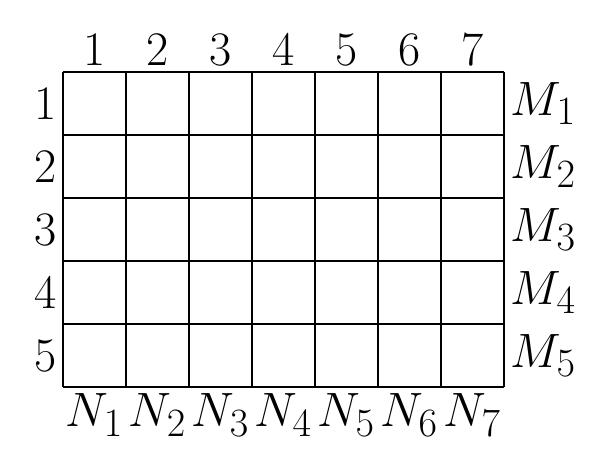
\begin{tikzpicture}[scale=0.8]  % Scale down by 80%
    % Define table size
    \def\nrow{5}  % Total rows
    \def\ncol{7}  % Total columns
    % Draw table grid lines on top
    \foreach \x in {0,...,\ncol} {
        \draw[thick] (\x,0) -- (\x,\nrow);
    }
    \foreach \y in {0,...,\nrow} {
        \draw[thick] (0,\y) -- (\ncol,\y);
    }
    % Labels for row sums (smaller text)
    \foreach \y in {1,...,\nrow} {
        \node[right,scale=0.7] at (\ncol,\nrow-\y+0.5) {\Huge $M_{\y}$};
    }
    % Labels for column sums (below table, smaller text)
    \foreach \x in {1,...,\ncol} {
        \node[below,scale=0.7] at (\x-0.5,0) {\Huge $N_{\x}$};
    }
    % Table numbering (row numbers on the left, smaller text)
    \foreach \y in {1,...,\nrow} {
        \node[left,scale=0.7] at (0,\nrow-\y+0.5) {\Huge \y};
    }
    % Column numbering (above table, smaller text)
    \foreach \x in {1,...,\ncol} {
        \node[above,scale=0.7] at (\x-0.5,\nrow) {\Huge \x};
    }
\end{tikzpicture}
\end{center}
\end{frame}

\begin{frame}
	\frametitle{Comparing distributions}
	%{\bf\underline{Example}} \par
	What if our table was larger?
    \begin{center}
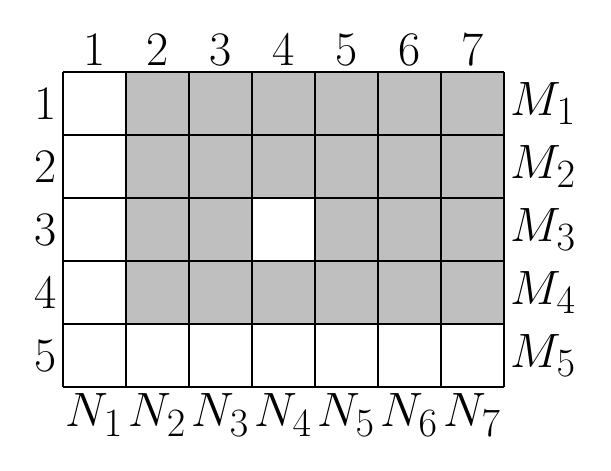
\begin{tikzpicture}[scale=0.8]  % Scale down by 80%
    % Define table size
    \def\nrow{5}  % Total rows
    \def\ncol{7}  % Total columns
    % Shade the (nrow-1) x (ncol-1) area (first 4 rows and 6 columns)
    \foreach \x in {1,...,6} {
        \foreach \y in {1,...,4} {
            \fill[gray!50] (\x,\y) rectangle ++(1,1);
        }
    }
    % Highlight one specific cell darker
    \fill[white] (3,2) rectangle ++(1,1);
    % Draw table grid lines on top
    \foreach \x in {0,...,\ncol} {
        \draw[thick] (\x,0) -- (\x,\nrow);
    }
    \foreach \y in {0,...,\nrow} {
        \draw[thick] (0,\y) -- (\ncol,\y);
    }
    % Labels for row sums (smaller text)
    \foreach \y in {1,...,\nrow} {
        \node[right,scale=0.7] at (\ncol,\nrow-\y+0.5) {\Huge $M_{\y}$};
    }
    % Labels for column sums (below table, smaller text)
    \foreach \x in {1,...,\ncol} {
        \node[below,scale=0.7] at (\x-0.5,0) {\Huge $N_{\x}$};
    }
    % Table numbering (row numbers on the left, smaller text)
    \foreach \y in {1,...,\nrow} {
        \node[left,scale=0.7] at (0,\nrow-\y+0.5) {\Huge \y};
    }
    % Column numbering (above table, smaller text)
    \foreach \x in {1,...,\ncol} {
        \node[above,scale=0.7] at (\x-0.5,\nrow) {\Huge \x};
    }
\end{tikzpicture}
\end{center}
\end{frame}

\begin{frame}
	\frametitle{Comparing distributions}
	%{\bf\underline{Example}} \par
	{\color{black!40}
		Note: the $y_i$ are not independent - why? \par
	}
	Assume we have $\bar x_1,\bar x_2,\dots,\bar x_{k-1}$ - then $\bar x_k=k-\sum_{i=1}^{k-1}\bar x_k$ \par
	%{\small\color{NavyBlue} - in fact, each time we add a variable to the sum, we loose ``freedom" in the remaining variables owing to the reduced population available}\par
	{\bf\underline{Theorem} (not proved in MATH163):} \par
	\begin{eqnarray*}
		\mathcal{X}^2:&=&\sum_{i=1}^k\frac{(\bar x_i-E[X_i])^2}{E[X_i]}\\
		&\xrightarrow{\text{$d$}}&\sum_{j=1}^{k-1}z_j^2\qquad\text{as}\ n\rightarrow\infty\\
		\text{where}\ \ z_j&\sim& N(0,1)\ \forall j
	\end{eqnarray*}
	This is a $\chi^2$ distribution with $n-1$ ``degrees of freedom" \par
	{\small\color{NavyBlue} - recall the idea of ``degrees of freedom" when defining the sample variance: we lose a degree of freedom by using sample data to approximate a population parameter \par
		- note the denominator in our statistic is equal to expectation, not variance}
\end{frame}

\begin{frame}
	\frametitle{Comparing distributions}
	Let $Y$ be a random variable, $Y\in\{1,2,\dots,k\},\ p_i:=P(Y=i)$ \par % so $\sum_{i=1}^k p_i=1$ \par
	Let $Y_1,Y_2,\dots,Y_n$ be independent observations of $Y$ \par%i.d.d. random variables sampled from the distribution of $Y$ \par
	{\small\color{NavyBlue} - pick $n$ numbers between $1$ and $k$, choosing number $i$ with probability $p_i$ \par
		- think of rolling a $k$ sided dice $n$ times where the dice may be biased}\par
	%{\bf We think $Y$ follows a PMF $P(Y=i)=p_i$, but we are not sure} \par
	Let $c_i$ be the number of values equal to $i$, so $c_i\in\{0,1,\dots, n\}\ \forall i$ \par
	{\small\color{NavyBlue} - count how many times each value occurs}\par
	WLLN $\implies\ \frac{c_i}{n}\rightarrow p_i$, or $c_i\rightarrow p_i n$, as $n\rightarrow\infty$ \par
	CLT $\implies$ $$\frac{\frac{c_i}{n}-p_i}{p_i}\sim N(0,1)$$ \par
	%What if we test using results for all values of $i$?
\end{frame}

\begin{frame}
	\frametitle{Tables of values}
	
\end{frame}

\begin{frame}
	\frametitle{Estimating parameters} 
	
\end{frame}
\end{comment}

%%%%%%%%%%%%%%%%%%%%%%%%%%%%%%%%%%%%%%%%%%%%%%%%%%%%%%%%%%%%%%%%
%%%%%%%%%%%%%%%%%%%%%%%%%%%%%%%%%%%%%%%%%%%%%%%%%%%%%%%%%%%%%%%%

\section{Week 10: statistical testing III}

\begin{frame}
	\frametitle{The $t$-distribution} 
	Recall the CLT: If $X$ has mean $\mu$ and variance $\sigma^2<\infty$ then:
	$$Z:=\frac{\bar X_n-\mu}{\sigma/\sqrt n}\sim N(0,1)\ \text{in the limit as}\ n\rightarrow \infty$$
	{\small\color{NavyBlue} - here the subscript ``$n$" denotes ``samples of size $n$"} \par
	We can use this to test a hypothesized population mean $\mu_0$ \par
	- but what if we don't know $\sigma^2$? \par
	We can approximate $\sigma$ with $S$ as follows:
	$$T:=\frac{\bar X_n-\mu}{S_n/\sqrt n}$$
	- but how is this distributed?
\end{frame}

\begin{frame}
	\frametitle{The $t$-distribution} 
	\begin{eqnarray*}
		T:&=&\frac{\bar X_n-\mu}{S_n/\sqrt n}=\frac{\bar X_n-\mu}{\sigma/\sqrt n}\times\frac{\sigma}{S_n}\\
		V:&=&(n-1)\frac{S_n^2}{\sigma^2}\sim\chi^2_{n-1}\\
		\Rightarrow T&=&Z\sqrt{\frac{n-1}{V}}\sim t_{n-1}
	\end{eqnarray*}
	{\small\color{NavyBlue} - ``$T$ follows a $t$-distribution with $n-1$ degrees of freedom" \par
		- the formula for the PDF of $T$ is disgusting \par
		- we require the fact that $Z$ and $V$ are independent}
\end{frame}

\begin{frame}
	\frametitle{The $t$-distribution}
	\begin{columns}
		\column{0.5\textwidth}
		\centering
		\fbox{\includegraphics[width=\textwidth]{tdist.png}}
		$t$-distribution PDF
		\column{0.5\textwidth}
		\centering
		\fbox{\includegraphics[width=\textwidth]{tcdf.png}}
        $t$-distribution CDF
	\end{columns}
\end{frame}

\begin{frame}
	\frametitle{Single sample $t$-tests} 
	Why $n-1$ degrees of freedom?
    \begin{itemize}
        \item The $n-1$ correction in $S^2$ yields an unbiased estimator of $\sigma^2$
        \item This is still an estimate, introducing additional uncertainty into the test statistic
        \item Variability in $S^2$ is still manifest in the denominator of $T$, which propagates to larger variance than when $\sigma^2$ is known
    \end{itemize}
\end{frame}

\begin{frame}
	\frametitle{Single sample $t$-tests} 
	Protocol: as with a $z$-test except:
    \begin{itemize}
        \item Use $S^2$ in place of $\sigma^2$ \par
        Warning:
        \begin{eqnarray*}
            S^2:&=&\frac 1{n-1}\sum_{i=1}^n(X_i-\bar X)^2 \\
            &=&\frac 1{n-1}\left(\sum_{i=1}^nX_i^2-2\sum_{i=1}^nX_i+\sum_{i=1}^n\bar X\right)\\
            &=&\frac 1{n-1}\left(\sum_{i=1}^nX_i^2-2n\bar X+n\bar X\right)\\
            &=&\frac 1{n-1}\sum_{i=1}^nX_i^2-\frac n{n-1}\bar X^2
        \end{eqnarray*}
        - this is not quite the ``mean of the square minus the square of the mean"
        \item Probabilities are calculated from the Student's $t$-distribution \par
        {\bf with $n-1$ degrees of freedom}
    \end{itemize}
\end{frame}

\begin{frame}
	\frametitle{Single sample $t$-tests} 
	Protocol: as with a $z$-test except:
    \begin{enumerate}
        \item State $H_0$
        \item State your alternate hypothesis $H_1$
        \item State your significance level ($100\alpha\%$)
        \item Calculate the sample mean $\bar x$, the sample variance $s^2$ and the $t$-statistic:
        $$t:=\frac{\bar x-\mu_0}{s/\sqrt{n}}$$
        \item Find the critical value $t^*_{n-1,\alpha}$ that corresponds to your significance level \par
        ($n-1$ denotes the degrees of freedom in the $t$-distribution)
        \item Do we reject $H_0$?
    \end{enumerate}
    Note: $t$-tables are different from normal tables: they provide critical $t$-values for given significance levels \par
    - this is because we have an extra parameter, namely degrees of freedom
\end{frame}

\begin{frame}
	\frametitle{Example 1} 
	How important is i to use the $t$-distribution over the normal distribution? \par
    A researcher is studying the effects of a new tutoring program on student test scores. A small sample of \( n = 8 \) students is selected, and their test score improvements (points gained after tutoring) are recorded in a frequency table:

    \[
\begin{array}{r|cccc}
\hline
\text{Improvement points} & 3 & 4 & 5 & 6 \\
\hline
\text{Frequency} & 1 & 3 & 2 & 2 \\
\hline
\end{array}
\]
A national study found that, on average, students improve by \( 4 \) points without tutoring. The researcher wants to determine whether the new tutoring program significantly improves scores.
\end{frame}

\begin{frame}
	\frametitle{Example 1}
    We have:
    \begin{eqnarray*}
        H_0:&&\ \mu\leq 4;\ H_1:\ \mu>4 \\
        \bar{x} &=& \frac 18(3 \times 1 + 4 \times 3 + 5 \times 2 + 6 \times 2)\\
        &=& 4.625 \\
        s^2 &=& \frac 17(3^2 \times 1 + 4^2 \times 3 + 5^2 \times 2 + 6^2 \times 2)-\frac 78\times\bar x^2\\%\frac{\sum_{i=1}^n (x_i - \bar{x})^2}{n-1}\\
        &=& 1.125 \\
        t &=& \frac{\bar x - \mu_0}{s / \sqrt{n}}\\
        &=& \frac{4.625 - 4}{\sqrt{1.125/8}} \\
        &=& 1.667 \\
        t^*_{7,0.05}&=& 1.895 \\
        z^*_{0.05}&=& 1.25 \\
    \end{eqnarray*}
    Conclusion: fail to reject $H_0$ at the 5\% significance level \par
    But what if we had done a $z$-test using $s^2$ in place of $\sigma^2$?
	%\color{red}
    %Warning: the next calculation illustrates an incorrect approach because we do not know $\sigma^2$ \par 
\end{frame}

\begin{frame}
	\frametitle{Approximate normality}
    {\bf Warning: working with small sample sizes ($n<30$) requires the population to be approximately normally distributed} \par
    The $t$-distribution accounts for additional variation in sample means due to estimating population variance \par
    We still rely on the CLT, so we need a large sample size ($n\geq 30)$ OR an (approximately) normally distributed population \par
    {\bf It is in small samples where the difference between $t$- and $z$-statistics is most apparent} \par
    When we have ($n<30$) and we have non-normality, non-parametric tests must be used \par
    How can we test for normality?
\end{frame}

\begin{frame}
	\frametitle{Confience intervals} 
	With unknown population variance, we also use the $t$-distribution to calculate confidence interval \par
    At confidence level $100(1-\alpha)\%$, we define:
    \begin{eqnarray*}
        CI_{1-\alpha}&=&\left(\bar x-t^*_{n-1,\frac{\alpha}{2}}\frac s{\sqrt n},\bar x+t^*_{n-1,\frac{\alpha}{2}}\frac s{\sqrt n}\right) \\
        \text{where}\quad s&=&\sqrt{\frac 1{n-1}\sum_{i=1}^nx_i^2-\frac n{n-1}\bar x^2}
    \end{eqnarray*}

    
\end{frame}

\begin{frame}
	\frametitle{Example 2}
    {\bf\underline{Question}} \\
    A business analyst is studying the relationship between sales revenue and profit margins. The analyst collects data from 5 small businesses and records their weekly sales revenue (in thousands of dollars). The data is presented in the following table:
    \begin{table}[h]
        \centering
        \begin{tabular}{r|ccccc}
            \hline
            Business & 1 & 2 & 3 & 4 & 5 \\
            \hline
            Sales (\$1000s) & 10 & 12 & 15 & 8 & 14 \\
            \hline
        \end{tabular}
    \end{table}
    Profit is calculated from sales revenue: there is a fixed cost of $2000$ when sales are zero, and that each additional $1000$ in sales contributes $600$ to profit after accounting for variable costs
    \begin{enumerate}
        \item Compute the sample mean \( \bar{X} \) and standard deviation \( s_X \) of the sales values
        \item Let $Y$ denote profit. Use a transformation formula to find \( \bar{Y} \) and \( s_Y \)
        \item Construct a 95\% confidence interval for the mean of \( Y \), assuming the data follows a normal distribution
        \item Justify the use of the Student’s t-distribution in this context
    \end{enumerate}
\end{frame}

\begin{frame}
	\frametitle{Example 2}
    {\bf\underline{Answer}} \\
    Note: \( Y = 0.6X - 2 \) so $\bar y=0.6\bar x-2$ and \( s_Y = 0.6^2 s_X \)
    \begin{eqnarray*}
        \bar{x} &=& \frac{10 + 12 + 15 + 8 + 14}{5} = \frac{59}{5} = 11.8 \\
        s_X^2 &=& \frac 14((10 - 11.8)^2 + (12 - 11.8)^2 + (15 - 11.8)^2 + (8 - 11.8)^2 + (14 - 11.8)^2) \\
        &=& \frac{32.8}{4} = 8.2 \\
        s_X &=& \sqrt{8.2} = 2.863 \\
        %Y &=& 0.6X - 2 \\
        \bar{y} &=& 0.6(11.8) - 2 = 7.08 - 2 = 5.08 \\
        s_Y^2 &=& (0.6)^2 s_X^2 = 0.36(8.2) = 2.952 \\
        s_Y &=& \sqrt{2.952} = 1.718
    \end{eqnarray*}
\end{frame}

\begin{frame}
	\frametitle{Example 2}
    {\bf\underline{Answer}} \\
    Using the Student's t-distribution with \( df = n-1 = 4 \) degrees of freedom, the critical value from the t-table for 95\% confidence is \( t^* = 2.776 \) \par
    The confidence interval is:
    \begin{eqnarray*}
        \left(\bar{y}-t^*\times\frac{s_Y}{\sqrt{n}},\quad \bar{y}+t^*\times\frac{s_Y}{\sqrt{n}}\right)=(2.94, 7.22)
    \end{eqnarray*}
    Justification: the population variance of profit is unknown, and the sample size is small (\( n < 30 \)), making the use of the Student’s $t$-distribution appropriate rather than the normal distribution \\
    Note: in this question, the table had one column per data point - not a frequency!
\end{frame}

\begin{frame}
	\frametitle{Example 3}
    {\bf\underline{Question}} \\
    A researcher is studying the effectiveness of a new training program on the success rate of students passing an exam. A random sample of 8 students was selected, and the number of students who passed the exam after completing the training program was recorded. The data is presented in the frequency table below:

\[
\begin{array}{r|ccc}
\hline
\text{Number of Passes} & 0 & 1 & 2 \\
\hline
\text{Frequency} & 2 & 3 & 3 \\
\hline
\end{array}
\]
The researcher hypothesizes that the average number of successful passes is 1
\begin{enumerate}
    \item Test the hypothesis at the 5\% significance level
    \item Now, multiply the sample size by 100, maintaining the relative frequencies, and perform the test again. Switch to a z-test for the larger sample size. How does the result change?
\end{enumerate}
\end{frame}

\begin{frame}
	\frametitle{Example 3}
    {\bf\underline{Answer}} \\
    $H_0$: $\mu=1$; $H_1$: $\mu\neq 1$
    \begin{eqnarray*}
        \bar{x} &=& \frac{2(0) + 3(1) + 3(2)}{2 + 3 + 3} = \frac{0 + 3 + 6}{8} = \frac{9}{8} = 1.125 \\
        s^2 &=& \frac{2(0 - 1.125)^2 + 3(1 - 1.125)^2 + 3(2 - 1.125)^2}{8 - 1}=0.696 \\
        s &=& 0.835 \\
        t &=& \frac{\bar{X} - \mu_0}{s / \sqrt{n}} = \frac{1.125 - 1}{0.8345 / \sqrt{8}} = \frac{0.125}{0.295} = 0.424 \\
        df &=& 8 - 1 = 7 \\
        t^*_{7,0.975} &=& 2.365>0.424
    \end{eqnarray*}
    - so we fail to reject $H_0$
\end{frame}

\begin{frame}
	\frametitle{Example 3}
    {\bf\underline{Answer}} \\
    Multiplying the frequencies by $100$ gives:
    \[
\begin{array}{r|ccc}
\hline
\text{Number of Passes} & 0 & 1 & 2 \\
\hline
\text{Frequency} & 200 & 300 & 300 \\
\hline
\end{array}
\]
$\bar x$ and $s$ remain unchanged, but $n$ is now much larger:
$$t=\frac{\bar{X} - \mu_0}{s / \sqrt{n}} = \frac{1.125 - 1}{0.835 / \sqrt{800}} = \frac{0.125}{0.030} = 4.237$$
We have $z^*_{0.95}=1.96<4.237,\ t^*_{799,0.975}=1.963<4.237$ so now we reject $H_0$
\end{frame}

\begin{frame}
	\frametitle{Further applications}
    %Variants of the $t$-test exist for comparing $2$ samples \par
    %- have these $2$ samples come from the same population? \par
    %The framework is very similar but you will not be assessed on this in MATH163
    The t-distribution is not only useful for one-sample tests and CIs, but also has several other applications in statistical inference \par
    Some key applications include:
    \begin{itemize}
        \item \textbf{One-Sample t-Test}: Testing the mean of a single sample against a known value when the population variance is unknown
        \item \textbf{Two-Sample t-Test}: Comparing the means of two independent samples to test if they come from the same population or have different means
        \item \textbf{Paired t-Test}: Comparing the means of two related groups (e.g., before and after treatment for the same subjects)
        %\item \textbf{Confidence Intervals for Means}: Constructing confidence intervals around the sample mean when the population variance is unknown
        \item \textbf{Regression Analysis}: In simple linear regression, the t-distribution is used to test the significance of regression coefficients
    \end{itemize}
    These will not be studied in MATH163
\end{frame}

\begin{frame}
	\frametitle{$\bigstar$ Statistical testing: summary} 
	You have a sample and a question regarding the sample \par
	Are you testing a single summary statistic (the mean)?
	\begin{itemize}
		\item {\bf YES:} \par
            Do you have a large sample size ($n\geq 30$) OR and approximately normal population?
		\begin{itemize}
			\item {\bf YES:} 
                    Do you know the population variance?
                    \begin{itemize}
                        \item {\bf YES:} $z$-test
                        \item {\bf YES:} $t$-test ($n-1$ degrees of freedom) - approximate $\sigma^2$ with $S^2$
                    \end{itemize}
			\item {\bf NO:} Non-parametric test (not in MATH163)
		\end{itemize}
		\item {\bf NO:} $\chi^2$-test\par
		Do you have a $2\times 2$ contingency table?
		\begin{itemize}
			\item {\bf YES:} Use {\it may} use the quick method
			\item {\bf NO:} Write out the expression for a $\mathcal{X}^2$ statistic
		\end{itemize}
	\end{itemize}
	%Note: there are $4$ possible approaches to take here. \par
	Across assessments, you will have to perform of all of these tests \par
	%{\bf You may not be told which test to use}
\end{frame}

\begin{comment}
1/2 tail test/which type of chi squared - comes from wording of H0

\end{comment}

\end{document}
\begin{comment}
\begin{frame}
	\frametitle{Some problem}
	\only<beamer>{Solution}
	\only<article>{\vskip10cm}
\end{frame}

\begin{frame}
	\frametitle{}
	\begin{itemize}
	\end{itemize}
\end{frame}

\begin{frame}[t]
	\frametitle{Transforming random variables}
	{\footnotesize
		\begin{columns}
			\column{0.55\textwidth}
			$Z=g(X),\ f_X(x)$ known
			\begin{enumerate}
				\item Compute CDF of $X$: \par
				$F_X(x)=P(X\leq x)$
				\item Write $F_Z(z)$ in terms of $X$: \par
				$P(Z\leq z)=P(g(X)\leq z)$\par
				$\qquad =F_X(g^{-1}(z))$
				\item Rearrange inequality in terms of $X$: \par
				$P(Z\leq z)=P(X\leq g^{-1}(z))$
				\item Differentiate w.r.t. $z$: \par
				$f_Z(z)=\frac d{dx}F_Z(z))$ \par
				$\qquad\ \ =\frac d{dx}F_X(g^{-1}(z))$
			\end{enumerate}
			
			\column{0.45\textwidth}
			\color{yellow}{
				$Z=x^2+1,\ f_X(x)=e^{-\lambda x},\ x\geq 0$}
			\begin{enumerate}
				\color{yellow}{
					\item $F_X(x)=\int_0^{\infty}e^{-\lambda t}dt$ \par
					$\qquad\quad\ =\frac 1{\lambda}(1-e^{-\lambda x})$
					\item $P(Z\leq z)=P(X^2+1\leq z)$ \par
					$\ $
					\item $P(Z\leq z)=P(X\leq \sqrt{z-1})$ \par
					$\qquad\qquad\ =\frac 1{\lambda}(1-e^{-\lambda\sqrt{z-1}})$ 
					\item 
					$f_Z(z)=\frac d{dx}F_Z(z)$ \par
					$\qquad\ \ =\frac 1{\lambda}\frac d{dx}(1-e^{-\lambda\sqrt{z-1}})$ \par
					$\qquad\ \ =\dots ,\ z\geq 1$
				}
			\end{enumerate}
		\end{columns}
		Question: why does this trick work?
		%Answer: CDF monotone increasing, ...
	}
\end{frame}

\end{comment}

\begin{comment}
		% Definition of circles
		%\def\firstcircle{(0,0) circle (1.5cm)}
		%\def\secondcircle{(0:2cm) circle (1.5cm)}
		\begin{columns}
			\column{.6\textwidth}
			
			\def\firstcircle{(0,0) circle (1cm)}
			\def\secondcircle{(0:1.25cm) circle (1cm)}
			\colorlet{circle edge}{NavyBlue!50}
			\colorlet{circle area}{NavyBlue!20}
			\tikzset{filled/.style={fill=circle area, draw=circle edge, thick},
				outline/.style={draw=circle edge, thick}}
			\setlength{\parskip}{5mm}
			% Set A or B
			
			\begin{tikzpicture}
				\draw[filled] \firstcircle node {$A$}
				\secondcircle node {$B$};
				\node[anchor=south] at (current bounding box.north) {$A \cup B$};
				\node[anchor=north] at (current bounding box.south) {Union};
			\end{tikzpicture}
			% Set A and B
			\begin{tikzpicture}
				\begin{scope}
					\clip \firstcircle;
					\fill[filled] \secondcircle;
				\end{scope}
				\draw[outline] \firstcircle node {$A$};
				\draw[outline] \secondcircle node {$B$};
				\node[anchor=south] at (current bounding box.north) {$A \cap B$};
				\node[anchor=north] at (current bounding box.south) {Intersection};
			\end{tikzpicture}
			
			%Set A or B but not (A and B) also known a A xor B
			\begin{tikzpicture}
				\draw[filled, even odd rule] \firstcircle node {$A$}
				\secondcircle node{$B$};
				\node[anchor=south] at (current bounding box.north) {$\overline{A \cap B}=\overline A\cup\overline B$};
				\node[anchor=north] at (current bounding box.south) {Complement};
			\end{tikzpicture}
			% Set A but not B
			\begin{tikzpicture}
				\begin{scope}
					\clip \firstcircle;
					\draw[filled, even odd rule] \firstcircle node {$A$}
					\secondcircle;
				\end{scope}
				\draw[outline] \firstcircle
				\secondcircle node {$B$};
				\node[anchor=south] at (current bounding box.north) {$A - B=A\cap\overline B$};
				\node[anchor=north] at (current bounding box.south) {Set difference};
			\end{tikzpicture}
			%\column{.3\textwidth}
			%\huge{
				%$$\mapsto[0,1]$$
				%}
		\end{columns}
        \end{comment}